\NeedsTeXFormat{LaTeX2e}
% twoside: needed for double-sided printing (odd/even pages)
\documentclass[12pt,twoside,a4paper]{article}
\raggedbottom
% includehead/headheight/headsep: reserve room for the page header
\usepackage[a4paper,
inner=3cm,    % Lề gáy sách: trang lẻ là lề trái, trang chẵn là lề phải
outer=2cm,    % Lề mép ngoài: trang lẻ là lề phải, trang chẵn là lề trái
top=2.5cm,
bottom=2.5cm,
headheight=15pt]{geometry}
\usepackage{amsmath,amsfonts,amssymb,amsthm}
\usepackage[utf8]{vietnam}
\usepackage{graphicx}
\usepackage[american]{circuitikz}
\usepackage{float}
\usepackage{mathptmx}
\usepackage{multicol}
\usepackage{enumitem} 
\usepackage{tasks} 
\usepackage{booktabs}
\usepackage{array}
\usepackage{caption}
\usepackage{hyperref}
\usepackage{pgfplots}
\usepackage{fancyhdr} % NEW: page header

\everymath{\displaystyle}
\theoremstyle{definition}
\newtheorem{bt}{} 
\renewcommand{\thebt}{\textbf{\large Q\arabic{bt}}} 

\newcommand{\bb}[1]{\mathbb{#1}}

\newlist{questions}{enumerate}{1}
\setlist[questions]{label=\textbf{Q$_{\mathbf{\arabic*}}$:}, leftmargin=4em}

\settasks{label=\textbf{\Alph*.}, label-width=1.5em, item-indent=7mm}
\pgfplotsset{compat=1.18}

%% =====================================================================
%% Additions for the combined document (everything above comes from the
%% original five files; everything below is new)
%% =====================================================================

\hypersetup{hidelinks}

% ---- Header / footer ------------------------------------------------
% Change the text below to whatever you want in the header.
\newcommand{\headertitle}{Physics II Experiment Report}

\pagestyle{fancy}
\fancyhf{}
\fancyhead[LO,RE]{\small\itshape\headertitle}   % inner side
\fancyhead[RO,LE]{\small\bfseries\rightmark}    % outer side: current experiment
\fancyfoot[C]{\small\thepage}
\renewcommand{\headrulewidth}{0.4pt}
\renewcommand{\footrulewidth}{0pt}

% ---- Blank pages inserted by \cleardoublepage carry no header/number --
\makeatletter
\def\cleardoublepage{\clearpage\if@twoside\ifodd\c@page\else
  \hbox{}\thispagestyle{empty}\newpage
  \if@twocolumn\hbox{}\newpage\fi\fi\fi}
\makeatother

% ---- Table of contents ---------------------------------------------
% Switch to \tocsectionsfalse to list only the experiments (no sections/subsections).
\newif\iftocsections
\tocsectionstrue

% Hiển thị tới cấp paragraph trong TOC:
%   \l@section       -> Experiment X: ... (Level 1)
%   \l@subsection    -> \section*         (Level 2: 1., 2., 3., ...)
%   \l@subsubsection -> \subsection*      (Level 3: 2.1., 2.2., ...)
%   \l@paragraph     -> \subsubsection*   (Level 4: 2.2.1., 3.1.1., ...)
\setcounter{tocdepth}{4}

\makeatletter
% 1. \section*{...} -> cấp subsection trong TOC
\let\orig@section\section
\renewcommand\section{\@ifstar\star@section\orig@section}
\newcommand\star@section[1]{%
	\iftocsections
	\phantomsection\addcontentsline{toc}{subsection}{#1}%
	\fi
	\orig@section*{#1}}

% 2. \subsection*{...} -> cấp subsubsection trong TOC
\let\orig@subsection\subsection
\renewcommand\subsection{\@ifstar\star@subsection\orig@subsection}
\newcommand\star@subsection[1]{%
	\iftocsections
	\phantomsection\addcontentsline{toc}{subsubsection}{#1}%
	\fi
	\orig@subsection*{#1}}

% 3. \subsubsection*{...} -> cấp paragraph trong TOC
\let\orig@subsubsection\subsubsection
\renewcommand\subsubsection{\@ifstar\star@subsubsection\orig@subsubsection}
\newcommand\star@subsubsection[1]{%
	\iftocsections
	\phantomsection\addcontentsline{toc}{paragraph}{#1}%
	\fi
	\orig@subsubsection*{#1}}

% TOC line styles: thụt lề tăng dần theo từng cấp
\renewcommand*\l@section[2]{%
	\addpenalty{-\@highpenalty}\addvspace{0.9em \@plus\p@}%
	\@dottedtocline{1}{0em}{6.6em}{\bfseries #1}{\bfseries #2}}
\renewcommand*\l@subsection{\@dottedtocline{2}{1.8em}{0em}}
\renewcommand*\l@subsubsection{\@dottedtocline{3}{3.6em}{0em}}
\renewcommand*\l@paragraph{\@dottedtocline{4}{5.4em}{0em}}
\makeatother

% ---- Experiments ----------------------------------------------------
% \StartExperiment{<number>}{<title shown in the TOC>}
%  * starts on an odd (right-hand) page
%  * resets Q / equation / figure / table numbering, because the text of
%    each experiment refers to them by hard-coded numbers
%  * sets the running header and adds the TOC / PDF-bookmark entry
\newcounter{expno}
\newcommand{\StartExperiment}[2]{%
  \cleardoublepage
  \setcounter{expno}{#1}%
  \setcounter{equation}{0}\setcounter{figure}{0}%
  \setcounter{table}{0}\setcounter{bt}{0}%
  \markboth{}{EXPERIMENT #1}%
  \phantomsection
  \addcontentsline{toc}{section}{\protect\numberline{Experiment #1:}#2}}

% unique hyperref anchors although the counters restart in each experiment
\def\theHequation{\arabic{expno}.\arabic{equation}}
\def\theHfigure{\arabic{expno}.\arabic{figure}}
\def\theHtable{\arabic{expno}.\arabic{table}}
\def\theHbt{\arabic{expno}.\arabic{bt}}

\begin{document}

%% =====================================================================
%% COVER PAGE (page 1, intentionally blank - design it later)
%% =====================================================================
\thispagestyle{empty}
\mbox{}

%% =====================================================================
%% =====================================================================
%% ABSTRACT (odd page)
%% =====================================================================
\cleardoublepage
\markboth{}{ABSTRACT}
\phantomsection\pdfbookmark[1]{ABSTRACT}{abstract}
\begin{center}
	\text{}
	
	\textbf{\Large ABSTRACT}
\end{center}
\vspace{0.5cm}

\noindent
This report summarizes five laboratory experiments conducted for the Physics II coursework, covering circuit analysis, electromagnetism, and electromagnetic wave propagation. 

\vspace{0.35cm}
\noindent
Using an oscilloscope and a function generator, the first experiment determines unknown resistance, capacitance, and inductance from phase-dependent Lissajous figures alongside the parallel and series resonant frequencies of an RLC circuit. 

\vspace{0.35cm}
\noindent
The second experiment maps the axial magnetic field of a finite solenoid as a function of position and current, benchmarking the results against the Biot--Savart--Laplace model. 

\vspace{0.35cm}
\noindent
Building on transient and oscillatory circuit behavior, the third experiment extracts coil resistance and inductance (with and without a core) from exponential current decay in an RL circuit and examines free damped oscillations and energy dissipation in an RLC circuit. 

\vspace{0.35cm}
\noindent
The fourth experiment investigates electromagnetic induction by recording voltage pulses generated as single and double bar magnets fall through 1200-turn and 150-turn coils.

\vspace{0.35cm}
\noindent
The final experiment examines microwave transmission through qualitative and quantitative tests—spanning rectilinear propagation, penetration, screening and absorption, reflection, refraction, diffraction, interference, and polarization—before determining microwave wavelength and frequency from standing-wave node/antinode spacing. 

\vspace{0.35cm}
\noindent
Across all five experiments, experimental readings are systematically tabulated, analyzed with error propagation, and interpreted in light of theoretical predictions.
%% =====================================================================
%% TABLE OF CONTENTS (odd page)
%% =====================================================================
\cleardoublepage
\markboth{}{TABLE OF CONTENTS}
\phantomsection\pdfbookmark[1]{TABLE OF CONTENTS}{toc}
\begin{center}
	\textbf{\Large TABLE OF CONTENTS}
\end{center}
\par
\vspace{0.3cm}
\makeatletter\@starttoc{toc}\makeatother

%% =====================================================================
%% EXPERIMENT 1  (content copied unchanged from Ex1-prefinal.tex)
%% =====================================================================
\StartExperiment{1}{Measurement of Resistance, Capacitance, Inductance and Resonant Frequencies of RLC Circuit Using Oscilloscope}
	\renewcommand{\figurename}{Figure}
	\renewcommand{\tablename}{Table}
	\begin{center}
		
		\textbf{\Large EXPERIMENT 1}
		
		\vspace{0.5cm}
		\textbf{{\Large MEASUREMENT OF RESISTANCE, CAPACITANCE,}}
		
		\vspace{0.15cm}
		\textbf{{\Large INDUCTANCE AND RESONANT FREQUENCIES}}
		
		\vspace{0.15cm}
		\textbf{{\Large OF RLC CIRCUIT USING OSCILLOSCOPE}}
	\end{center}
	\vspace{-0.5cm}
	\section*{1. Devices and Purpose of the experiment}
	\begin{center}
		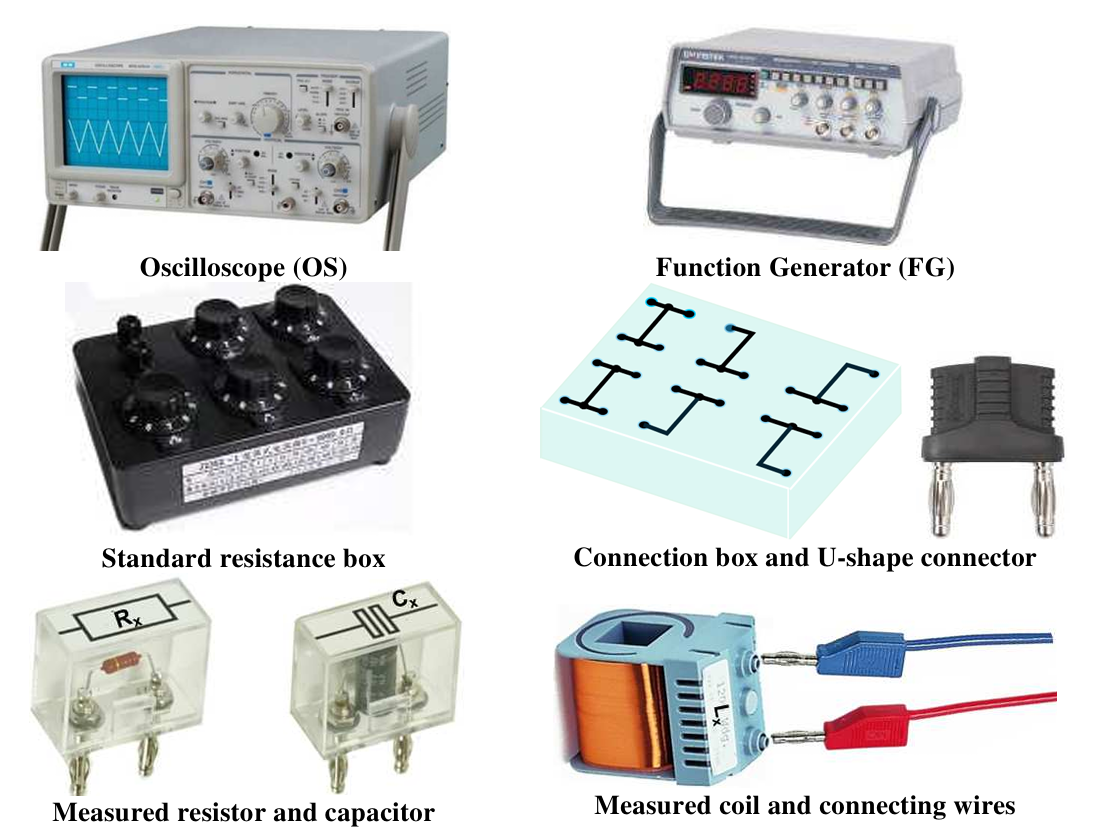
\includegraphics[width=0.8\textwidth]{Devices1}
		\captionof{figure}{\textit{ Measurement circuit layout (a), connection box with the notations (b)}}
	\end{center}
	
	\noindent
	The experiment helps the student understanding the typical RLC circuits and the manner to use the equipments including oscilloscope and function generator in electronic engineering, namely measuring the physical basic parameters like resistance, capacitance, and inductance as well as the resonant frequencies.
	
	\vspace{-0.5cm}
	\section*{2. Theoretical background}
	\subsection*{2.1. RLC Circuit}
	An RLC circuit (also known as a resonant circuit or a tuned circuit) is an electrical circuit consisting of a resistor ($R$), an inductor ($L$), and a capacitor ($C$), connected in series or in parallel. Every RLC circuit consists of two main components: a power source and a resonator (series LC or parallel LC).
	\begin{center}
		\begin{circuitikz}[american]
			\draw (0,0) to[sV, l=$E$] (0,2.5)
			to[R, l=$R$] (5,2.5)
			to[L, l=$L$] (5,0)
			to[C, l=$C$] (0,0);
			
			\draw (7.5,0) to[sV, l=$E$] (7.5,2.5)
			to[R, l=$R$] (10.5,2.5)
			to[short] (12.5,2.5);
			\draw (10.5,2.5) to[C, l=$C$] (10.5,0);
			\draw (12.5,2.5) to[L, l=$L$] (12.5,0);
			\draw (12.5,0) to[short] (7.5,0);
		\end{circuitikz}
		\captionof{figure}{\textit{Series (left) and parallel (right) RLC circuit }}
	\end{center}
	The undamped resonance or natural angular frequency of an $LC$ circuit (in $\text{rad/s}$) is given by:
	\begin{equation}
		\omega_{_0} = \frac{1}{\sqrt{LC}}
	\end{equation}
	In the more familiar unit of Hz (or $\text{s}^{-1}$), the natural frequency becomes:
	\begin{equation}
		f_0 = \frac{\omega_{_0}}{2\pi} = \frac{1}{2\pi\sqrt{LC}}
	\end{equation}
	Resonance occurs in an RLC circuit when the complex impedance $Z_{LC}$ of the $LC$ resonator becomes zero:
	\begin{equation}
		Z_{LC} = Z_L + Z_C = 0
	\end{equation}
	At this condition, the applied frequency matches the resonant frequency $f_0$ of the RLC circuit.
	
	\vspace{0.5cm}
	\noindent
	The damping factor $\beta$ (in $\text{rad/s}$) for a series RLC circuit is:
	\begin{equation}
		\beta = \frac{R}{2L}
	\end{equation}
	and for a parallel RLC circuit:
	\begin{equation}
		\beta = \frac{1}{2RC}
	\end{equation}
	
	\subsection*{2.2. Oscilloscope}
	\subsubsection*{2.2.1. General description}
	An oscilloscope (OS) is an electronic test instrument that allows signal voltages to be viewed as a two-dimensional graph of electrical potential differences. The simplest type of OS consists of a cathode ray tube (CRT), a vertical amplifier, a time-base, a horizontal amplifier, and a power supply. The vertical amplifier generates a potential difference $U_y$ across one pair of plates $Y_1Y_2$, giving rise to a vertical electric field through which the electron beam passes. In general, the amplifier has a very high input impedance, typically one MW, so that it draws only a tiny current from the signal source. The horizontal amplifier does a similar job with the other pair of deflection plates $U_1U_2$, causing the 
	beam to move left or right by potential difference $U_x$. In general, when switched on, a CRT normally displays a single bright dot in the center of the screen.
	\begin{center}
		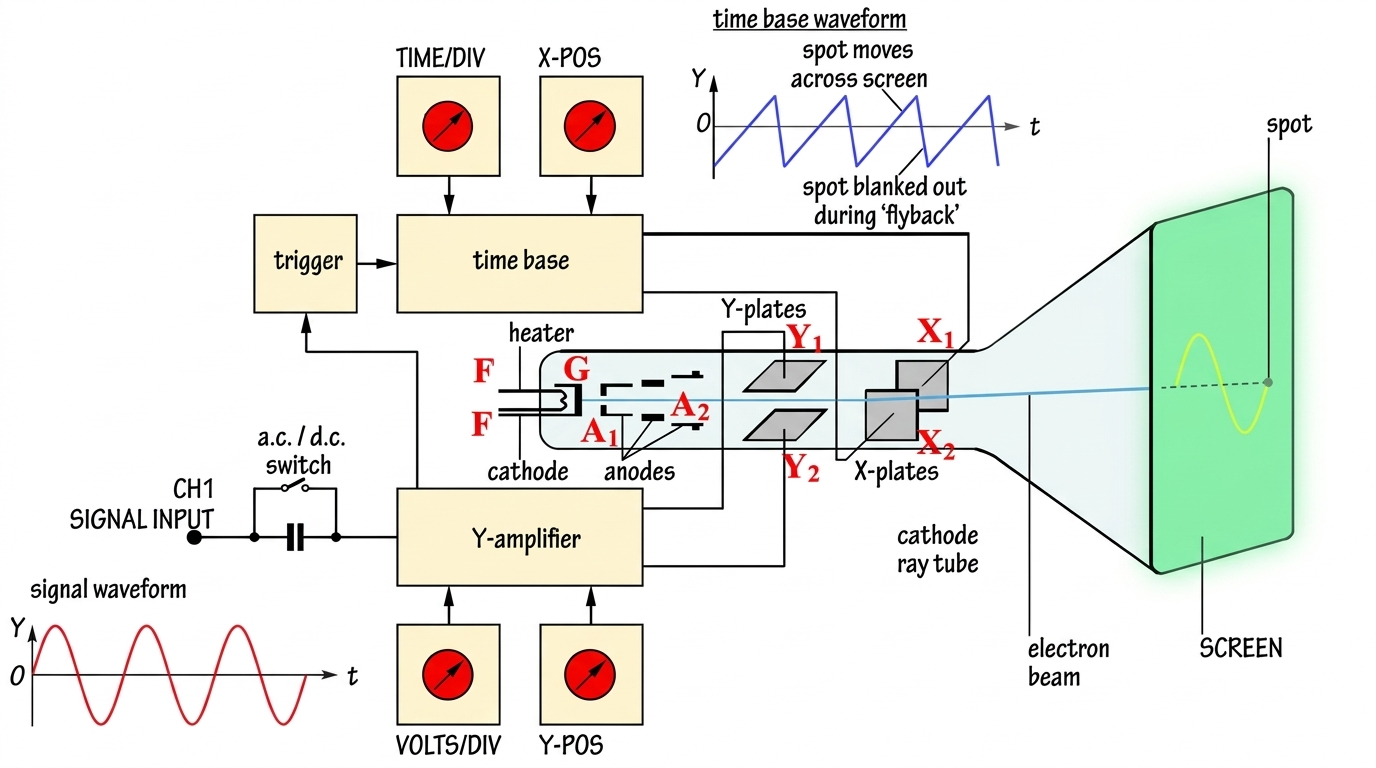
\includegraphics[width=0.8\textwidth]{OS1}
		\captionof{figure}{\textit{ Principle structure of an oscilloscope}}
	\end{center}
	
	
	\vspace{0.5cm}
	\hspace{-0.73cm}
	Assuming an input signal $U_y$ is applied to the vertical deflection plates $Y_1 Y_2$ (Y-channel):
	\begin{equation}
		U_y = U_{0y} \cos(\omega t)
	\end{equation}
	Similarly, when $U_x$ is applied to the horizontal deflection plates $X_1 X_2$ (X-channel):
	\begin{equation}
		U_x = U_{0x} \cos(\omega t)
	\end{equation}
	There is a knob on the front panel of the oscilloscope for adjusting the sweep frequency. This knob allows keeping the 
	value of $U_0$ and $U_\text{max}$ constant and changing the sweep speed, 
	consequently the sweep frequency and the slope of graph $U_x$. By adjusting this knob so that $T_s = nT$, $n$ stable total 
	oscillations can be observed on the screen.
	
	\subsubsection*{2.2.2. Resultant signal form produced by two perpendicular oscillations}
	If alternating voltages $U_x = U_{0x} \cos(\omega_x t)$ and $U_y = U_{0y} \cos(\omega_y t + \varphi)$ are applied simultaneously to the X-channel and Y-channel plates, respectively, the electron beam traces the superposition of two perpendicular oscillations:
	\begin{equation}
		\begin{aligned}
			&x = K_x U_x = x_0 \cos(\omega_x t) \\
			&y = K_y U_y = y_0 \cos(\omega_y t + \varphi)
		\end{aligned}
	\end{equation}
	When $\omega_x = \omega_y$ ($n = 1$), the trace on the screen follows the ellipse equation:
	\begin{equation}
		\left(\frac{x}{x_0}\right)^2 + \left(\frac{y}{y_0}\right)^2 - 2\frac{xy}{x_0 y_0}\cos\varphi = \sin^2\varphi
	\end{equation}
	\newpage
	Depending on the phase difference $\varphi$, the trace takes specific geometric forms:
	\begin{itemize}[leftmargin=1.5cm]
		\item If $\varphi = 0$ or $\varphi = \pi$, a \textbf{diagonal line} is displayed, corresponding to a purely resistive circuit or an RLC circuit at resonance ($Z_L + Z_C = 0$).
		\item If $\varphi = \pm \frac{\pi}{2}$, an \textbf{upright oval} is displayed, corresponding to an RC or RL circuit. When $U_{0x} = U_{0y}$ (i.e., $R_0 = Z_C$ or $R_0 = Z_L$), the trace becomes a \textbf{circle}.
		\item For an arbitrary phase difference $\varphi$, the trace is an \textbf{oblique oval}, corresponding to a general RLC circuit off resonance.
	\end{itemize}
	\begin{center}
		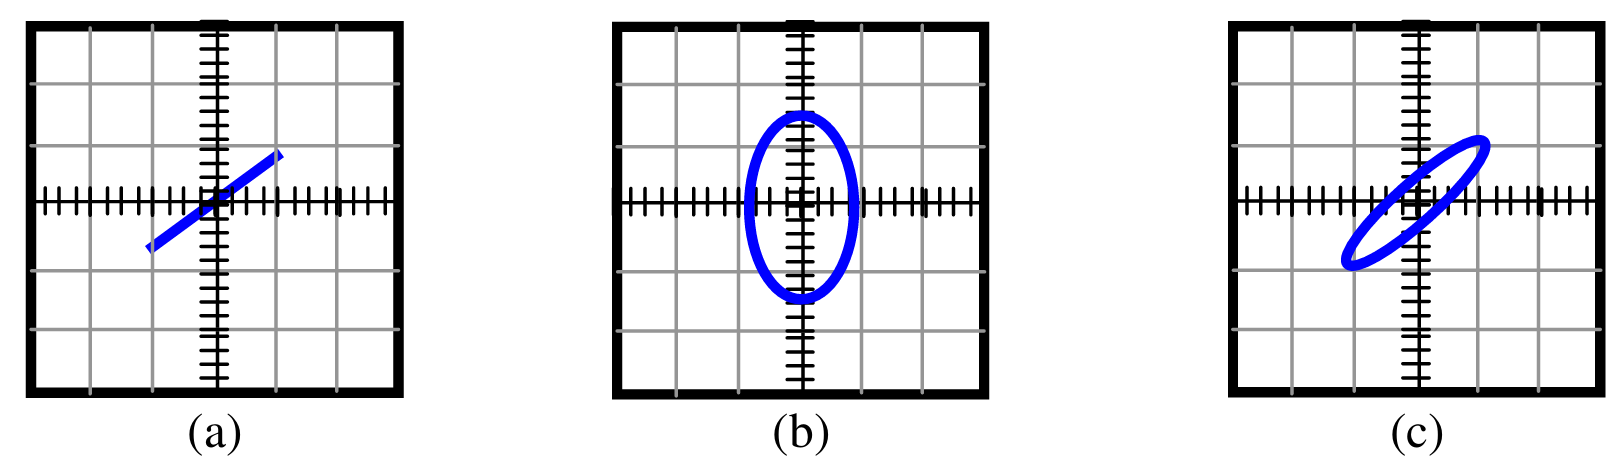
\includegraphics[width=0.8\textwidth]{SignalForm}
		\captionof{figure}{\textit{ Signal forms on oscilloscope screen produced by two perpendicular oscillations}}
	\end{center}
	
	\subsection*{2.3. Function Generator and Component Determination}
	A function generator (FG) produces repetitive waveforms (such as sine, square, and triangular waves) to stimulate the circuit under test.
	\begin{center}
		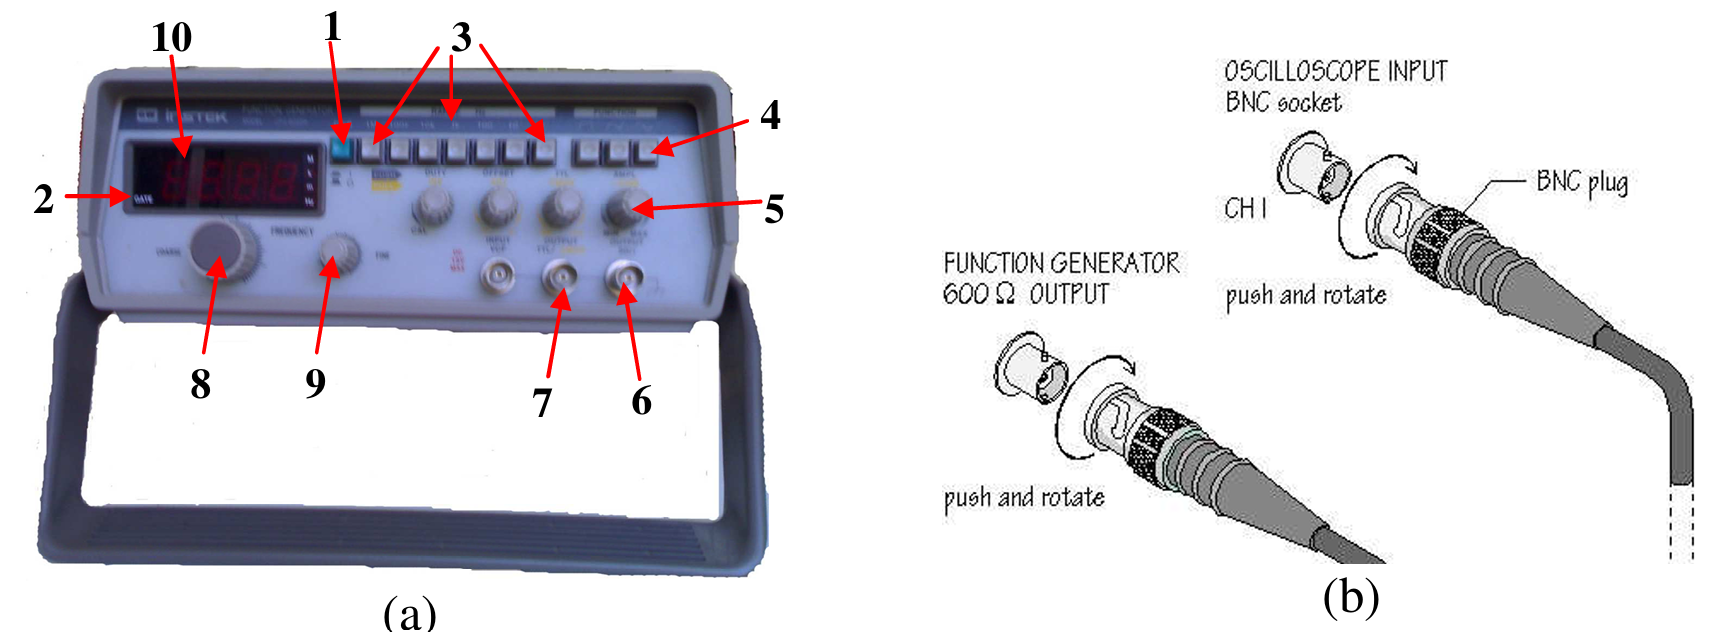
\includegraphics[width=0.8\textwidth]{FuncGen}
		\captionof{figure}{\textit{ Front panel of function generator GF8020F (a) and BNC connector (b)}}
		\textit{1. On/off power switch; 2 and 10. LED display; 3. Scale buttons of generated frequency range; 4. Button for output option of sine waveform; 5. Adjustor for output voltage amplitude; 8. Adjustor for rough frequency; 9. Adjustor for fine frequency.}
	\end{center}
	
	\vspace{0.5cm}
	\hspace{-0.73cm}
	When measuring an unknown capacitor $C_X$ in series with a standard resistance box $R_0$, adjusting $R_0$ until the upright oval becomes a circle yields $U_{C_X} = U_{R_0}$, so:
	\begin{equation}
		Z_C = \frac{1}{2\pi f C_X} = R_0 \implies C_X = \frac{1}{2\pi f R_0}
	\end{equation}
	Similarly, when measuring an unknown inductor $L_X$ in series with $R_0$, obtaining a circular trace gives $U_{L_X} = U_{R_0}$, so:
	\begin{equation}
		Z_L = 2\pi f L_X = R_0 \implies L_X = \frac{R_0}{2\pi f}
	\end{equation}
	
	\section*{3. Experimental procedure}
	
	\subsection*{3.1. Measurement of Resistance, Capacitance, and Inductance}
	\begin{center}
		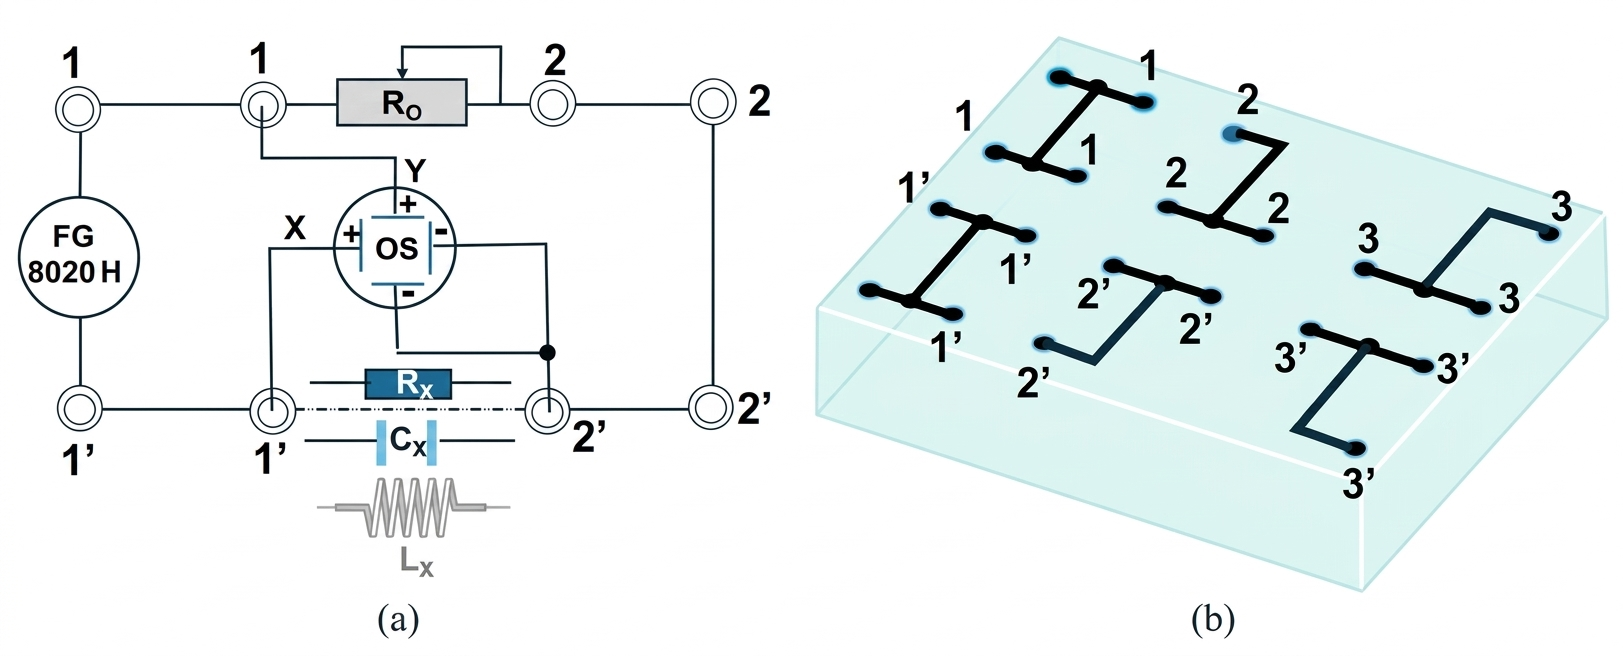
\includegraphics[width=\textwidth]{RLC measure}
		\captionof{figure}{\textit{ Measurement circuit layout (a), connection box with the notations (b)}}
	\end{center}
	\subsubsection*{3.1.1. Measurement of unknown resistance ($R_X$)}
	\begin{enumerate}[leftmargin=1.5em]
		\item Connect the Function Generator (FG) output to terminals $1$ and $1'$ of the connection box. Set FG to sine wave output at an initial frequency of $500\text{ Hz}$ (or $1000\text{ Hz}$).
		\item Connect the standard resistance box $R_0$ between points $1$ and $2$, the unknown resistor $R_X$ between points $1'$ and $2'$, and a U-shape connector between points $2$ and $2'$.
		\item Connect the OS X-channel to points $1'$ and $2'$, and the Y-channel to points $1$ and $2$. Center the trace on the OS screen.
		\item Adjust $R_0$ (from higher to lower decade knobs) until the vertical line becomes a diagonal line ($U_X = U_Y \implies R_X = R_0$). Record $f$ and $R_0$ in Table 1.
		\item Reset $R_0$ to zero and repeat the measurement for two additional frequencies (e.g., $1000\text{ Hz}$ and $1500\text{ Hz}$, or $1500\text{ Hz}$ and $2000\text{ Hz}$).
	\end{enumerate}
	
	\subsubsection*{3.1.2. Measurement of unknown capacitance ($C_X$)}
	\begin{enumerate}[leftmargin=1.5em]
		\item Replace $R_X$ with the unknown capacitor $C_X$ between points $1'$ and $2'$, and set FG frequency to $1000\text{ Hz}$.
		\item Center the upright oval trace on the OS screen and adjust $R_0$ until the oval becomes a circle. Record $f$ and $R_0$ in Table 2, then calculate $C_X$ using Eq. (11).
		\item Reset $R_0$ to zero and repeat for $2000\text{ Hz}$ and $3000\text{ Hz}$.
	\end{enumerate}
	
	\subsubsection*{3.1.3. Measurement of unknown inductance ($L_X$)}
	\begin{enumerate}[leftmargin=1.5em]
		\item Replace $C_X$ with the unknown coil $L_X$ between points $1'$ and $2'$, and set FG frequency to $10000\text{ Hz}$.
		\item Center the upright oval trace on the OS screen and adjust $R_0$ until the oval becomes a circle. Record $f$ and $R_0$ in Table 3, then calculate $L_X$ using Eq. (12).
		\item Reset $R_0$ to zero and repeat for $20000\text{ Hz}$ and $30000\text{ Hz}$.
	\end{enumerate}
	
	\subsection*{3.2. Measurement of Resonant Frequency of RLC Circuit}
	\subsubsection*{3.2.1. Parallel RLC circuit}
	\begin{enumerate}[leftmargin=1.5em]
		\item Connect $R_0$ ($1000\,\Omega$) between points $1$ and $2$. Insert U-shape connectors across $(2,3)$, $(2',3')$, and $(1',2')$. Connect both $C_X$ and $L_X$ in parallel across points $3$ and $3'$. Connect OS X-channel to $(1,1')$ and Y-channel to $(2,2')$.
		\item Adjust the FG frequency knobs until the oblique oval on the OS screen collapses into an inclined straight line. Record the parallel resonant frequency $f_p$ in Table 4.
		\item Repeat the measurement two more times to obtain three trials.
	\end{enumerate}
	\begin{figure}[H]
		\centering
		\begin{circuitikz}[american, line width=0.8pt]
			% Định nghĩa kiểu nút giắc cắm (vòng tròn đôi)
			\tikzset{
				jack/.style={draw, circle, inner sep=0pt, minimum size=12pt, fill=white,
					path picture={\draw (path picture bounding box.center) circle (3.5pt);}}
			}
			
			% 1. Khung dây nhánh trên: 1 -> 1 -> R_0 -> 2 -> 3 -> 3
			\draw (0,0) -- (0,4) -- (2.2,4)
			to[european potentiometer, l_=$R_0$] (5.8,4)
			-- (8.5,4) -- (11,4);
			
			% 2. Khung dây nhánh dưới: 1' -> 1' -> 2' -> 3' -> 3'
			\draw (0,0) -- (2.2,0) -- (5.8,0) -- (8.5,0) -- (11,0);
			
			% 3. Hai nhánh mắc song song: Tụ C_x (tại x=8.5) và Cuộn cảm L_x (tại x=11)
			\draw (8.5,4) to[C, l_=$C_x$] (8.5,0);
			\draw (11,4)  to[L, l=$L_x$]  (11,0);
			
			% 4. Máy phát tần số FG 8020 H (bên trái)
			\node[draw, circle, fill=white, minimum size=1.6cm, align=center, font=\bfseries\small] at (0,2) {FG\\8020 H};
			
			% 5. Dao động ký OS (gồm 4 bản cực lệch hướng và dấu +, -)
			\begin{scope}[shift={(4,2)}]
				\draw[fill=white] (0,0) circle (0.85cm);
				\node[font=\bfseries\small] at (0,0) {OS};
				% 4 bản cực bên trong
				\draw[thick] (-0.3, 0.42) -- (0.3, 0.42);   % Y+
				\draw[thick] (-0.3,-0.42) -- (0.3,-0.42);   % Y-
				\draw[thick] (-0.42,-0.3) -- (-0.42, 0.3);  % X+
				\draw[thick] ( 0.42,-0.3) -- ( 0.42, 0.3);  % X-
				% Dấu cực tính (+ / -)
				\node[font=\bfseries\scriptsize] at ( 0.25, 0.62) {+};
				\node[font=\bfseries\scriptsize] at ( 0.25,-0.62) {-};
				\node[font=\bfseries\scriptsize] at (-0.62, 0.25) {+};
				\node[font=\bfseries\scriptsize] at ( 0.62, 0.25) {-};
			\end{scope}
			
			% Dây nối từ các giắc cắm vào kênh X và Y của OS
			\draw (2.2,4) -- (2.2,2) -- (3.58,2);                  % Giắc 1 -> X+
			\node[font=\bfseries\small] at (3.0, 2.25) {X};
			
			\draw (5.8,4) -- (5.8,3.2) -- (4,3.2) -- (4,2.42);     % Giắc 2 -> Y+
			\node[font=\bfseries\small] at (3.65, 3.1) {Y};
			
			% Nối chung hai cực âm (X- và Y-) về giắc 2'
			\draw (4.42,2) -- (5.8,2) -- (5.8,0);                  % X- -> Giắc 2'
			\draw (4,1.58) -- (4,0.8) -- (5.8,0.8);                % Y- nối chung dây về 2'
			\fill (5.8,0.8) circle (2pt);                          % Chấm nối dây
			
			% 6. Vẽ tất cả các giắc cắm (vòng tròn đôi) đè lên trên dây và gắn nhãn
			\node[jack, label=above:{\textbf{1}}]  at (0,4) {};
			\node[jack, label=above:{\textbf{1}}]  at (2.2,4) {};
			\node[jack, label=above:{\textbf{2}}]  at (5.8,4) {};
			\node[jack, label=above:{\textbf{3}}]  at (8.5,4) {};
			\node[jack, label=above:{\textbf{3}}]  at (11,4) {};
			
			\node[jack, label=below:{\textbf{1'}}] at (0,0) {};
			\node[jack, label=below:{\textbf{1'}}] at (2.2,0) {};
			\node[jack, label=below:{\textbf{2'}}] at (5.8,0) {};
			\node[jack, label=below:{\textbf{3'}}] at (8.5,0) {};
			\node[jack, label=below:{\textbf{3'}}] at (11,0) {};
		\end{circuitikz}
		\caption{\textit{Parallel RLC circuit layout for measurement of resonant frequency}}
	\end{figure}
	
	\subsubsection*{3.2.2. Series RLC circuit}
	\begin{enumerate}[leftmargin=1.5em]
		\item Keep $R_0 = 1000\,\Omega$ across $(1,2)$ and U-shape connectors across $(2,3)$ and $(1',2')$. Move $C_X$ to points $(2',3')$ so that $C_X$ and $L_X$ (at $3,3'$) are connected in series. Keep OS connections unchanged.
		\item Vary the FG frequency until the oblique oval collapses into an inclined straight line. Record the series resonant frequency $f_s$ in Table 4.
		\item Repeat the measurement two more times to obtain three trials.
	\end{enumerate}
	\begin{figure}[H]
		\centering
		\begin{circuitikz}[american, line width=0.8pt]
			% Định nghĩa kiểu nút giắc cắm (vòng tròn đôi)
			\tikzset{
				jack/.style={draw, circle, inner sep=0pt, minimum size=12pt, fill=white,
					path picture={\draw (path picture bounding box.center) circle (3.5pt);}}
			}
			
			% 1. Khung dây nhánh trên: 1 -> 1 -> R_0 -> 2 -> 3 -> 3
			\draw (0,0) -- (0,4) -- (2.2,4)
			to[european potentiometer, l_=$R_0$] (5.8,4)
			-- (8.5,4) -- (11,4);
			
			% 2. Khung dây nhánh dưới: 1' -> 1' -> 2' -> C_x -> 3' -> 3'
			\draw (0,0) -- (2.2,0) -- (5.8,0)
			to[C, l=$C_x$] (8.5,0)
			-- (11,0);
			
			% 3. Nhánh cuộn cảm L_x mắc nối tiếp ở bên phải (giữa 3 và 3')
			\draw (11,4) to[L, l=$L_x$] (11,0);
			
			% 4. Máy phát tần số FG 8020 H (bên trái)
			\node[draw, circle, fill=white, minimum size=1.6cm, align=center, font=\bfseries\small] at (0,2) {FG\\8020 H};
			
			% 5. Dao động ký OS (gồm 4 bản cực lệch hướng và dấu +, -)
			\begin{scope}[shift={(4,2)}]
				\draw[fill=white] (0,0) circle (0.85cm);
				\node[font=\bfseries\small] at (0,0) {OS};
				% 4 bản cực bên trong
				\draw[thick] (-0.3, 0.42) -- (0.3, 0.42);   % Y+
				\draw[thick] (-0.3,-0.42) -- (0.3,-0.42);   % Y-
				\draw[thick] (-0.42,-0.3) -- (-0.42, 0.3);  % X+
				\draw[thick] ( 0.42,-0.3) -- ( 0.42, 0.3);  % X-
				% Dấu cực tính (+ / -)
				\node[font=\bfseries\scriptsize] at ( 0.25, 0.62) {+};
				\node[font=\bfseries\scriptsize] at ( 0.25,-0.62) {-};
				\node[font=\bfseries\scriptsize] at (-0.62, 0.25) {+};
				\node[font=\bfseries\scriptsize] at ( 0.62, 0.25) {-};
			\end{scope}
			
			% Dây nối từ các giắc cắm vào kênh X và Y của OS
			\draw (2.2,4) -- (2.2,2) -- (3.58,2);                  % Giắc 1 -> X+
			\node[font=\bfseries\small] at (3.0, 2.25) {X};
			
			\draw (5.8,4) -- (5.8,3.2) -- (4,3.2) -- (4,2.42);     % Giắc 2 -> Y+
			\node[font=\bfseries\small] at (3.65, 3.1) {Y};
			
			% Nối chung hai cực âm (X- và Y-) về giắc 2'
			\draw (4.42,2) -- (5.8,2) -- (5.8,0);                  % X- -> Giắc 2'
			\draw (4,1.58) -- (4,0.8) -- (5.8,0.8);                % Y- nối chung dây về 2'
			\fill (5.8,0.8) circle (2pt);                          % Chấm nối dây
			
			% 6. Vẽ tất cả các giắc cắm (vòng tròn đôi) đè lên trên dây và gắn nhãn
			\node[jack, label=above:{\textbf{1}}]  at (0,4) {};
			\node[jack, label=above:{\textbf{1}}]  at (2.2,4) {};
			\node[jack, label=above:{\textbf{2}}]  at (5.8,4) {};
			\node[jack, label=above:{\textbf{3}}]  at (8.5,4) {};
			\node[jack, label=above:{\textbf{3}}]  at (11,4) {};
			
			\node[jack, label=below:{\textbf{1'}}] at (0,0) {};
			\node[jack, label=below:{\textbf{1'}}] at (2.2,0) {};
			\node[jack, label=below:{\textbf{2'}}] at (5.8,0) {};
			\node[jack, label=below:{\textbf{3'}}] at (8.5,0) {};
			\node[jack, label=below:{\textbf{3'}}] at (11,0) {};
		\end{circuitikz}
		\caption{\textit{Series RLC circuit layout for measurement of resonant frequency}}
	\end{figure}
	
	\section*{4. Experimental results}
	\subsection*{4.1. Measurement of resistance, capacitance, and inductance}
	\subsubsection*{4.1.1. Data Tables}
	
	\begin{table}[H]
		\centering
		\caption{Measurement of unknown resistance $R_X$}
		\begin{tabular}{|>{\centering\arraybackslash}m{1.5cm}|>{\centering\arraybackslash}m{4.5cm}|>{\centering\arraybackslash}m{5.5cm}|}
			\hline
			\textbf{Trial} & \textbf{Frequency $f$ (Hz)} & \textbf{Standard Resistance $R_0$ ($\Omega$)} \rule[-0.2cm]{0pt}{0.6cm} \\
			\hline
			1 & 500 & 560 \rule[-0.25cm]{0pt}{0.7cm} \\
			\hline
			2 & 1000 & 557 \rule[-0.25cm]{0pt}{0.7cm} \\
			\hline
			3 & 1500 & 562 \rule[-0.25cm]{0pt}{0.7cm} \\
			\hline
		\end{tabular}
	\end{table}
	
	\begin{table}[H]
		\centering
		\caption{Measurement of unknown capacitance $C_X$}
		\begin{tabular}{|>{\centering\arraybackslash}m{1.5cm}|>{\centering\arraybackslash}m{4.5cm}|>{\centering\arraybackslash}m{5.5cm}|}
			\hline
			\textbf{Trial} & \textbf{Frequency $f$ (Hz)} & \textbf{Standard Resistance $R_0$ ($\Omega$)} \rule[-0.2cm]{0pt}{0.6cm} \\
			\hline
			1 & 1000 & 251  \rule[-0.25cm]{0pt}{0.7cm} \\
			\hline
			2 & 2000 & 133  \rule[-0.25cm]{0pt}{0.7cm} \\
			\hline
			3 & 3000 & 81  \rule[-0.25cm]{0pt}{0.7cm} \\
			\hline
		\end{tabular}
	\end{table}
	
	\begin{table}[H]
		\centering
		\caption{Measurement of unknown inductance $L_X$}
		\begin{tabular}{|>{\centering\arraybackslash}m{1.5cm}|>{\centering\arraybackslash}m{4.5cm}|>{\centering\arraybackslash}m{5.5cm}|}
			\hline
			\textbf{Trial} & \textbf{Frequency $f$ (Hz)} & \textbf{Standard Resistance $R_0$ ($\Omega$)} \rule[-0.2cm]{0pt}{0.6cm} \\
			\hline
			1 & 10007 & 60 \rule[-0.25cm]{0pt}{0.7cm} \\
			\hline
			2 & 20009 & 120 \rule[-0.25cm]{0pt}{0.7cm} \\
			\hline
			3 & 30004 & 161 \rule[-0.25cm]{0pt}{0.7cm} \\
			\hline
		\end{tabular}
	\end{table}
	
	\subsubsection*{4.1.2. Data processing}
	\textbf{{\normalsize For unknown resistance $R_X$}}
	
	\noindent	
	Since the traces obtained after 3 trials are diagonal lines, $U_X = U_Y = U_{R_0}, \text{ implying that } R_X = R_0$. Hence, the mean value of unknown resistance is
	\begin{center}
		\fbox{%
			\begin{minipage}{0.8\textwidth}
				\vspace{-0.4cm}
				\centering
				\begin{displaymath}
					\overline{R_X} = \frac{R_{X1} + R_{X2} + R_{X3}}{3} = \dfrac{560 + 557 + 562}{3} = \dfrac{1679}{3} \approx 559.667 \left(\Omega\right)
				\end{displaymath}
			\end{minipage}%
		}
	\end{center}
	
	\noindent
	The standard deviation of a single measurement is
	\begin{center}
		\fbox{%
			\begin{minipage}{0.8\textwidth}
				\vspace{-0.4cm}
				\centering
				\begin{displaymath}
					\text{sd} = \sqrt{\frac{\left(R_{X1} - \overline{R_X}\right)^2 + \left(R_{X2} - \overline{R_X}\right)^2 + \left(R_{X3} - \overline{R_X}\right)^2}{3}} = \dfrac{\sqrt{38}}{3} \left(\Omega\right)
				\end{displaymath}
			\end{minipage}%
		}
	\end{center}
	
	\noindent
	And the standard deviation of the mean is
	\begin{center}
		\fbox{%
			\begin{minipage}{0.8\textwidth}
				\vspace{-0.4cm}
				\centering
				\begin{displaymath}
					\text{SD} = \dfrac{\text{sd}}{\sqrt{3}} = \dfrac{\sqrt{114}}{9} \approx 1.186 \left(\Omega\right)
				\end{displaymath}
			\end{minipage}%
		}
	\end{center}
	
	\noindent
	Therefore, our result for $R_X$ appears as
	\begin{center}
		\fbox{%
			\begin{minipage}{0.8\textwidth}
				\vspace{-0.4cm}
				\centering
				\begin{displaymath}
					R_X = \overline{R_X} \pm \text{SD} = 559.667 \pm 1.186 \left(\Omega\right)
				\end{displaymath}
			\end{minipage}%
		}
	\end{center}			
	
	\noindent
	\textbf{For unknown capacitance $C_X$}
	
	\noindent
	Since the traces obtained after 3 trials are circles, $C_X = \frac{1}{2\pi f R_0}$. Hence, we have
	\begin{center}
		\fbox{%
			\begin{minipage}{0.8\textwidth}
				\vspace{-0.4cm}
				\centering
				\begin{displaymath}
					\begin{aligned}
						&C_{X1} = \dfrac{1}{2 \pi \times 1000 \times 251} \approx 6.341 \times 10^{-7} \left(\text{F}\right)\\
						&C_{X2} = \dfrac{1}{2 \pi \times 2000 \times 133} \approx 5.983 \times 10^{-7} \left(\text{F}\right)\\
						&C_{X3} = \dfrac{1}{2 \pi \times 3000 \times 81} \approx 6.550 \times 10^{-7} \left(\text{F}\right)
					\end{aligned}
				\end{displaymath}
			\end{minipage}%
		}
	\end{center}
	
	\noindent
	The mean value of unknown capacitance is
	\begin{center}
		\fbox{%
			\begin{minipage}{0.8\textwidth}
				\vspace{-0.4cm}
				\centering
				\begin{displaymath}
					\overline{C_X} = \frac{C_{X1} + C_{X2} + C_{X3}}{3} \approx \dfrac{6.341 + 5.983 + 6.550}{3} \times 10^{-7} \approx 6.291 \times 10^{-7} \left(\text{F}\right)
				\end{displaymath}
			\end{minipage}%
		}
	\end{center}
	
	\noindent
	The standard deviation of a single measurement is
	\begin{center}
		\fbox{%
			\begin{minipage}{0.8\textwidth}
				\vspace{-0.4cm}
				\centering
				\begin{displaymath}
					\text{sd} = \sqrt{\frac{\left(C_{X1} - \overline{C_X}\right)^2 + \left(C_{X2} - \overline{C_X}\right)^2 + \left(C_{X3} - \overline{C_X}\right)^2}{3}} \approx 0.234 \times 10^{-7} \left(\text{F}\right)
				\end{displaymath}
			\end{minipage}%
		}
	\end{center}
	
	\noindent
	And the standard deviation of the mean is
	\begin{center}
		\fbox{%
			\begin{minipage}{0.8\textwidth}
				\vspace{-0.4cm}
				\centering
				\begin{displaymath}
					\text{SD} = \dfrac{\text{sd}}{\sqrt{3}} \approx 0.135 \times 10^{-7} \left(\text{F}\right)
				\end{displaymath}
			\end{minipage}%
		}
	\end{center}
	
	\noindent
	Therefore, our result for $C_X$ appears as
	\begin{center}
		\fbox{%
			\begin{minipage}{0.8\textwidth}
				\vspace{-0.4cm}
				\centering
				\begin{displaymath}
					C_X = \overline{C_X} \pm \text{SD} = \left(6.291 \pm 0.135\right) \times 10^{-7} \left(\text{F}\right)
				\end{displaymath}
			\end{minipage}%
		}
	\end{center}
	
	\noindent
	\textbf{For unknown inductance $L_X$}
	
	\noindent
	Since the traces obtained after 3 trials are circles, $L_X = \frac{R_0}{2\pi f}$. Hence, we have
	\begin{center}
		\fbox{%
			\begin{minipage}{0.8\textwidth}
				\vspace{-0.4cm}
				\centering
				\begin{displaymath}
					\begin{aligned}
						&L_{X1} = \dfrac{60}{2 \pi \times 100007} \approx 9.543\times 10^{-4} \left(\text{H}\right)\\
						&L_{X2} = \dfrac{120}{2 \pi \times 20009} \approx 9.545 \times 10^{-4} \left(\text{H}\right)\\
						&L_{X3} = \dfrac{161}{2 \pi \times 30004} \approx 8.540 \times 10^{-4} \left(\text{H}\right)
					\end{aligned}
				\end{displaymath}
			\end{minipage}%
		}
	\end{center}
	
	\noindent
	The mean value of unknown inductance is
	\begin{center}
		\fbox{%
			\begin{minipage}{0.8\textwidth}
				\vspace{-0.4cm}
				\centering
				\begin{displaymath}
					\overline{L_X} = \frac{L_{X1} + L_{X2} + L_{X3}}{3} \approx \dfrac{9.543 + 9.545 + 8.540}{3} \times 10^{-4} \approx 9.209 \times 10^{-4} \left(\text{H}\right)
				\end{displaymath}
			\end{minipage}%
		}
	\end{center}
	
	\noindent
	The standard deviation of a single measurement is
	\begin{center}
		\fbox{%
			\begin{minipage}{0.8\textwidth}
				\vspace{-0.4cm}
				\centering
				\begin{displaymath}
					\text{sd} = \sqrt{\frac{\left(L_{X1} - \overline{L_X}\right)^2 + \left(L_{X2} - \overline{L_X}\right)^2 + \left(L_{X3} - \overline{L_X}\right)^2}{3}} \approx 0.473 \times 10^{-4} \left(\text{H}\right)
				\end{displaymath}
			\end{minipage}%
		}
	\end{center}
	
	\noindent
	And the standard deviation of the mean is
	\begin{center}
		\fbox{%
			\begin{minipage}{0.8\textwidth}
				\vspace{-0.4cm}
				\centering
				\begin{displaymath}
					\text{SD} = \dfrac{\text{sd}}{\sqrt{3}} \approx 0.273 \times 10^{-4} \left(\text{H}\right)
				\end{displaymath}
			\end{minipage}%
		}
	\end{center}
	
	\noindent
	Therefore, our result for $L_X$ appears as
	\begin{center}
		\fbox{%
			\begin{minipage}{0.8\textwidth}
				\vspace{-0.4cm}
				\centering
				\begin{displaymath}
					L_X = \overline{L_X} \pm \text{SD} = \left(9.209 \pm 0.273\right) \times 10^{-4} \left(\text{H}\right)
				\end{displaymath}
			\end{minipage}%
		}
	\end{center}
	
	\subsection*{4.2. Resonant Frequencies of Parallel and Series RLC Circuits}
	\subsubsection*{4.2.1. Data table}
	\begin{table}[H]
		\centering
		\caption{Measurement of parallel and series resonant frequencies}
		\begin{tabular}{|>{\centering\arraybackslash}m{1.5cm}|>{\centering\arraybackslash}m{7cm}|>{\centering\arraybackslash}m{7cm}|}
			\hline
			\textbf{Trial} & \textbf{Parallel Resonant Frequency $f_p$ (Hz)} & \textbf{Series Resonant Frequency $f_s$ (Hz)} \rule[-0.2cm]{0pt}{0.6cm} \\
			\hline
			1 & 6568 & 6421 \rule[-0.25cm]{0pt}{0.7cm} \\
			\hline
			2 & 6570 & 6725 \rule[-0.25cm]{0pt}{0.7cm} \\
			\hline
			3 & 6572 & 6750 \rule[-0.25cm]{0pt}{0.7cm} \\
			\hline
		\end{tabular}
	\end{table}
	\subsubsection*{4.2.2. Data processing}
	
	\noindent
	The mean values of parallel resonant frequency and series resonant frequency are
	\begin{center}
		\fbox{%
			\begin{minipage}{0.8\textwidth}
				\vspace{-0.4cm}
				\centering
				\begin{displaymath}
					\begin{aligned}
						&\overline{f_p} = \frac{f_{p1} + f_{p2} + f_{p3}}{3} = \dfrac{6568 + 6570 + 6572}{3} = 6570 \left(\text{Hz}\right) \\
						&\overline{f_s} = \frac{f_{s1} + f_{s2} + f_{s3}}{3} = \dfrac{6421 + 6725 + 6750}{3} = 6632 \left(\text{Hz}\right)
					\end{aligned}
				\end{displaymath}
			\end{minipage}%
		}
	\end{center}
	
	\noindent
	The standard deviations of a single measurement for $f_p$ and $f_s$ are
	\begin{center}
		\fbox{%
			\begin{minipage}{0.8\textwidth}
				\vspace{-0.4cm}
				\centering
				\begin{displaymath}
					\begin{aligned}
						&\text{sd}_{f_p} = \sqrt{\frac{\left(f_{p1} - \overline{f_p}\right)^2 + \left(f_{p2} - \overline{f_p}\right)^2 + \left(f_{p3} - \overline{f_p}\right)^2}{3}} = \dfrac{2\sqrt{6}}{3} \left(\text{Hz}\right) \\
						&\text{sd}_{f_s} = \sqrt{\frac{\left(f_{s1} - \overline{f_s}\right)^2 + \left(f_{s2} - \overline{f_s}\right)^2 + \left(f_{s3} - \overline{f_s}\right)^2}{3}} \approx 149.548 \left(\text{Hz}\right)
					\end{aligned}
				\end{displaymath}
			\end{minipage}%
		}
	\end{center}
	
	\noindent
	And the standard deviations of the means for $f_p$ and $f_s$ are
	\begin{center}
		\fbox{%
			\begin{minipage}{0.8\textwidth}
				\vspace{-0.4cm}
				\centering
				\begin{displaymath}
					\begin{aligned}
						&\text{SD}_{f_p} = \dfrac{\text{sd}_{f_p}}{\sqrt{3}} \approx 0.943 \left(\text{Hz}\right) \\
						&\text{SD}_{f_s} = \dfrac{\text{sd}_{f_s}}{\sqrt{3}} \approx 86.342 \left(\text{Hz}\right)
					\end{aligned}
				\end{displaymath}
			\end{minipage}%
		}
	\end{center}
	
	\noindent
	Therefore, our result for $f_p$ and $f_s$ appear as
	\begin{center}
		\fbox{%
			\begin{minipage}{0.8\textwidth}
				\vspace{-0.4cm}
				\centering
				\begin{displaymath}
					\begin{aligned}
						&f_p = \overline{f_p} \pm \text{SD}_{f_p} = 6570.000 \pm 0.943 \left(\text{Hz}\right) \\
						&f_s = \overline{f_s} \pm \text{SD}_{f_s} = 6632.000 \pm 86.342 \left(\text{Hz}\right)
					\end{aligned}
				\end{displaymath}
			\end{minipage}%
		}
	\end{center}
	
	\begin{bt}
		\textit{Compare the measured average values of parallel ($\overline{f}_p$) and series ($\overline{f}_s$) resonant frequencies with the theoretical resonant frequency $f_0$ calculated using Eq. (2), and discuss sources of experimental error.}
		
		\vspace{0.2cm}
		\noindent
		From Eq. (2), the theoretical mean resonant frequency calculated from $\overline{L_X}$ and $\overline{C_X}$ is
		\begin{center}
			\fbox{%
				\begin{minipage}{0.8\textwidth}
					\vspace{-0.4cm}
					\centering
					\begin{displaymath}
						\overline{f_0} = \frac{1}{2\pi \sqrt{\overline{L}_X \overline{C}_X}} 
						= \dfrac{1}{2\pi \sqrt{\left(9.209 \times 10^{-4}\right) \times \left(6.291 \times 10^{-7}\right)}} \approx 6612.323 
						\left(\text{Hz}\right)
					\end{displaymath}
				\end{minipage}%
			}
		\end{center}
		
		\noindent
		By the propagation of uncertainty, the relative uncertainty in $\overline{f_0}$ is
		\begin{center}
			\fbox{%
				\begin{minipage}{0.8\textwidth}
					\vspace{-0.4cm}
					\centering
					\begin{displaymath}
						\dfrac{\Delta f_0}{\overline{f_0}} = \sqrt{\left(\dfrac{-1}{2} \times \dfrac{\Delta L_X}{\overline{L_X}}\right)^2 + \left(\dfrac{-1}{2} \times \dfrac{\Delta C_X}{\overline{C_X}}\right)^2} = \dfrac{1}{2} \times \sqrt{\left(\dfrac{\Delta L_X}{\overline{L_X}}\right)^2 + \left(\dfrac{\Delta C_X}{\overline{C_X}}\right)^2}
					\end{displaymath}
				\end{minipage}%
			}
		\end{center}
		
		\noindent
		And the uncertainty in $f_0$ is
		\begin{center}
			\fbox{%
				\begin{minipage}{0.8\textwidth}
					\vspace{-0.4cm}
					\centering
					\begin{displaymath}
						\Delta f_0 = \dfrac{\overline{f_0}}{2} \times \sqrt{\left(\dfrac{\Delta L_X}{\overline{L_X}}\right)^2 + \left(\dfrac{\Delta C_X}{\overline{C_X}}\right)^2} \approx 120.995 \left(\text{Hz}\right)
					\end{displaymath}
				\end{minipage}%
			}
		\end{center}
		
		\noindent
		Therefore, the theoretical resonant frequency $f_0$ is
		\begin{center}
			\fbox{%
				\begin{minipage}{0.8\textwidth}
					\vspace{-0.4cm}
					\centering
					\begin{displaymath}
						f_0 = \overline{f_0} \pm \Delta f_0 = 6612.323 \pm 120.995 \left(\text{Hz}\right)
					\end{displaymath}
				\end{minipage}%
			}
		\end{center}
		
		\noindent
		The measured average resonant frequencies $\overline{f}_p$ and $\overline{f}_s$ are in close agreement with the theoretical value $f_0 = \frac{1}{2\pi\sqrt{\overline{L}_X \overline{C}_X}}$. Any slight discrepancies arise from the non-zero internal ohmic resistance of the inductor coil (which shifts the damped parallel resonant frequency slightly below $f_0$), parasitic capacitance and inductance in the connecting wires, and visual judgment uncertainty when determining the exact collapse of the Lissajous ellipse into a straight line on the oscilloscope screen.
	\end{bt}
	

%% =====================================================================
%% EXPERIMENT 2  (content copied unchanged from Ex2-prefinal.tex)
%% =====================================================================
\StartExperiment{2}{Measurement of Magnetic Field inside a Solenoid with Finite Length}
	\renewcommand{\figurename}{Figure}
	\renewcommand{\tablename}{Table}
	
	\begin{center}
		\textbf{\Large EXPERIMENT 2}
		
		\vspace{0.5cm}
		\textbf{{\Large MEASUREMENT OF MAGNETIC FIELD INSIDE A}}
		
		\vspace{0.25cm}
		\textbf{{\Large SOLENOID WITH FINITE LENGTH}}
	\end{center}
	
	\section*{1.  Devices and Purpose of the experiment}
	\begin{center}
		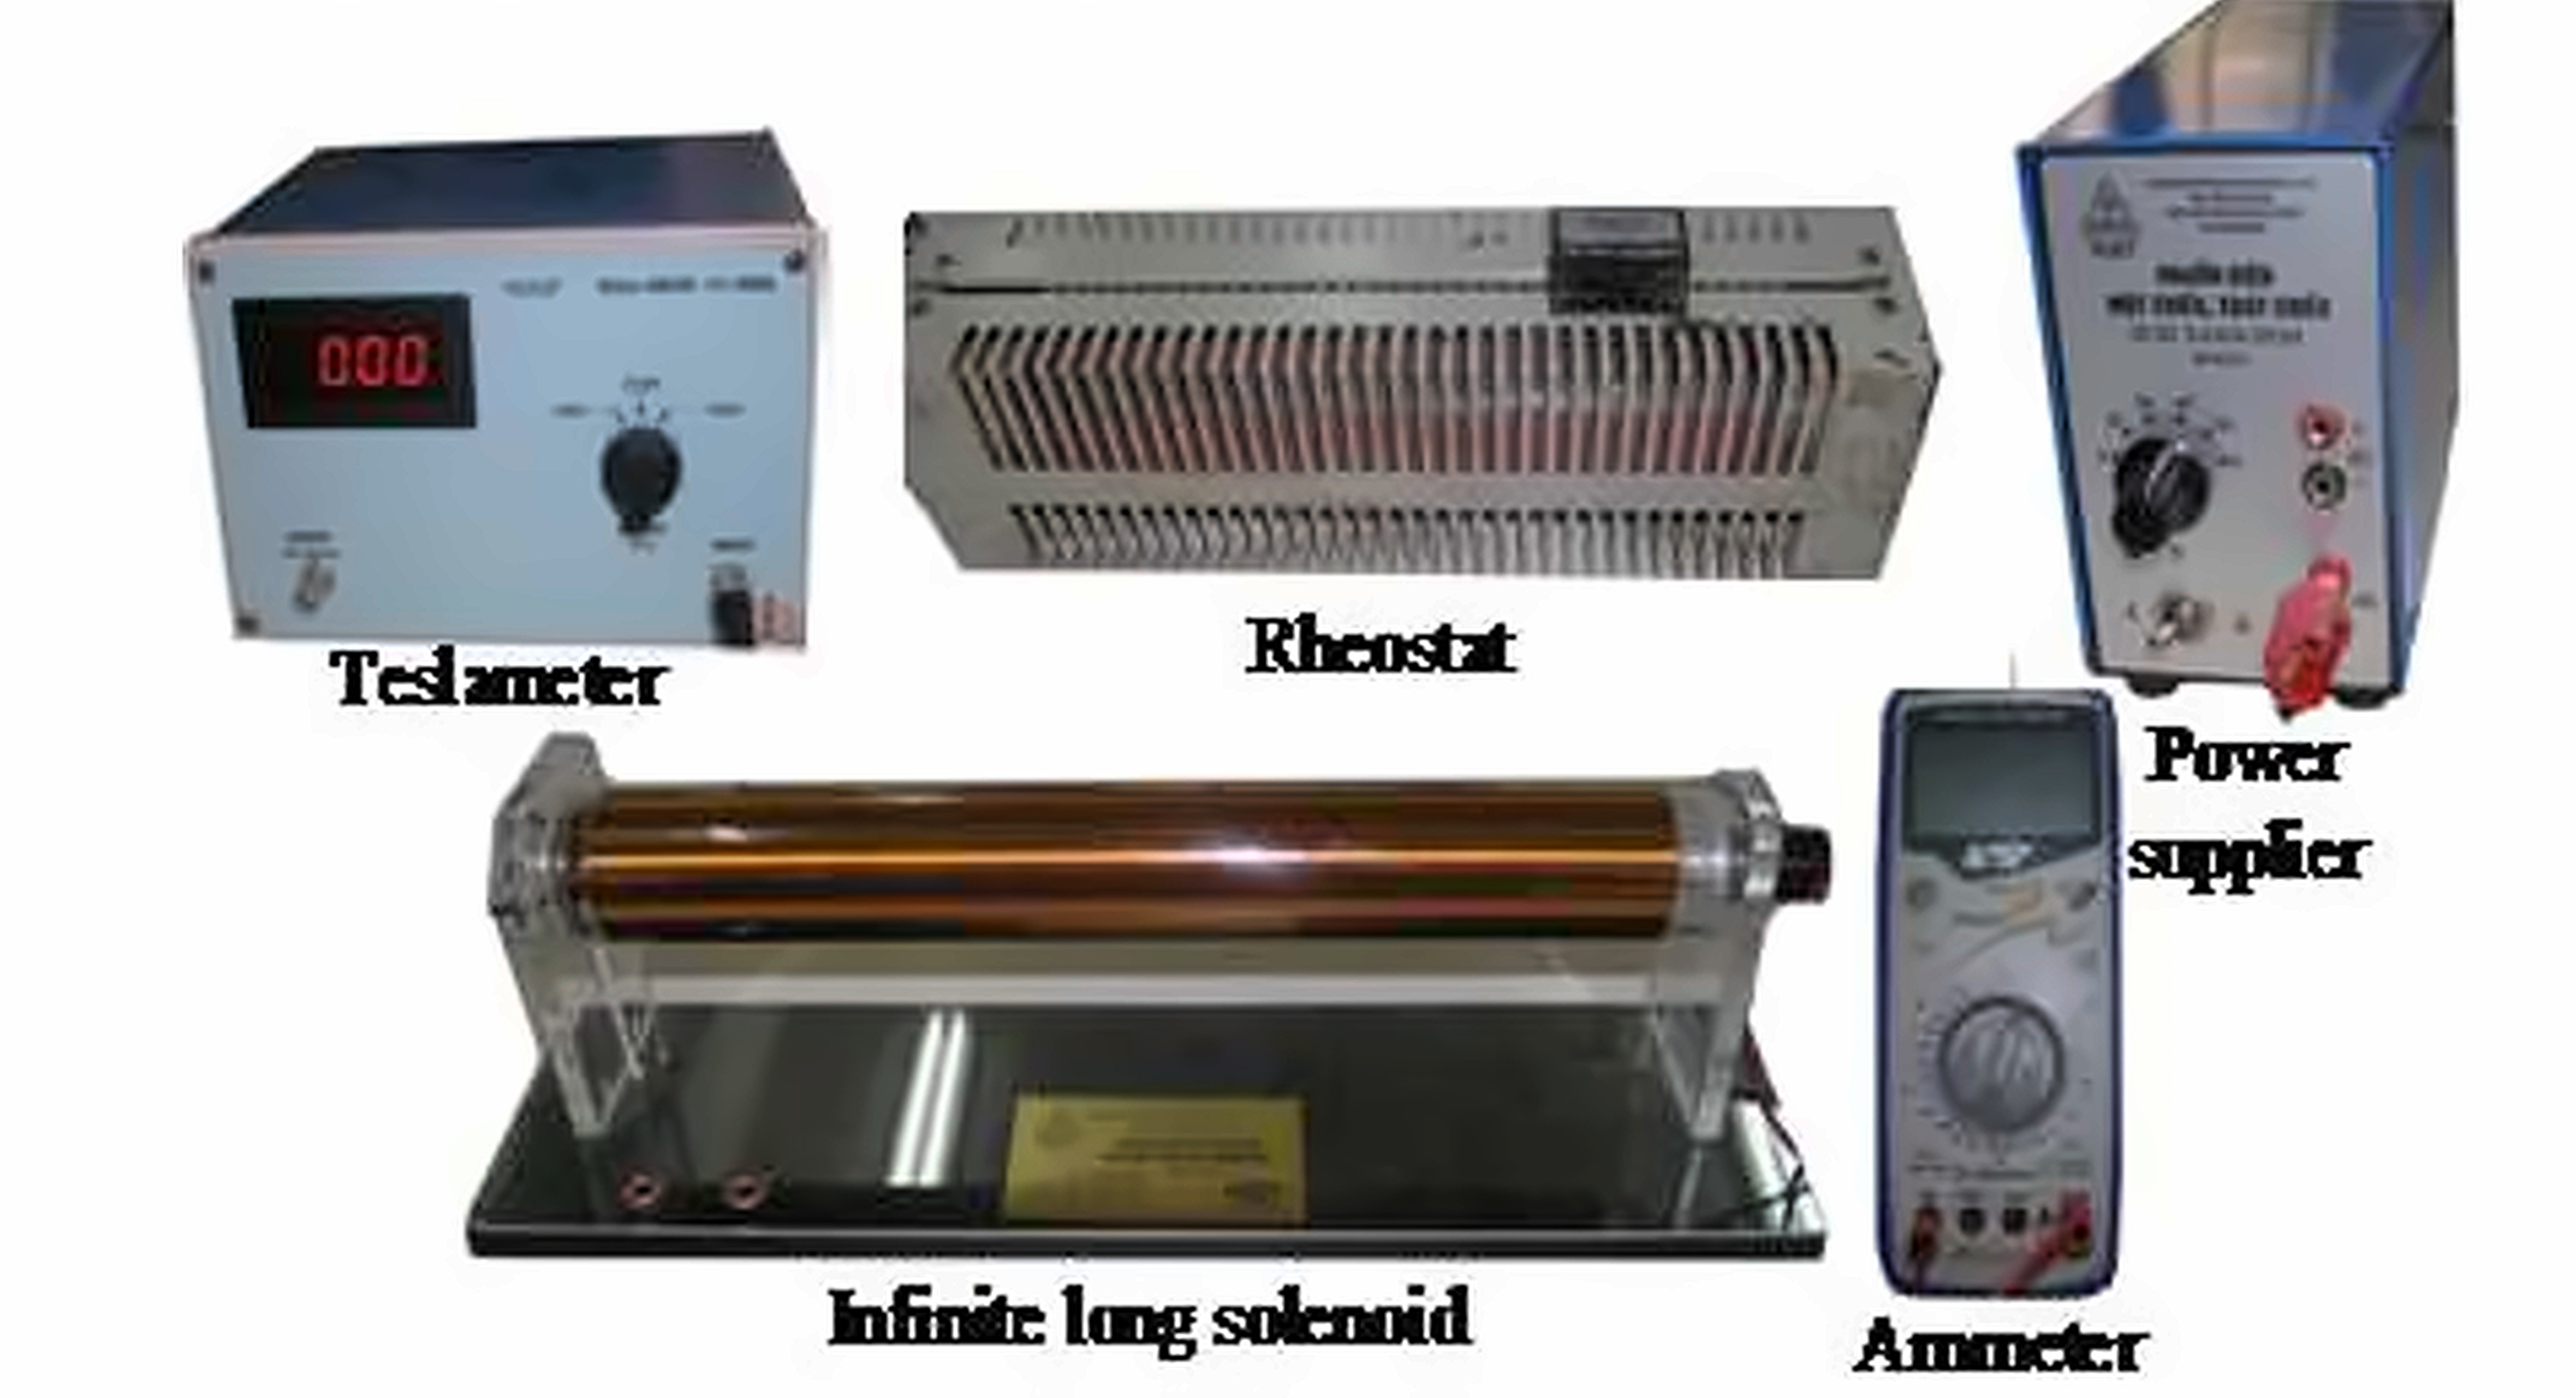
\includegraphics[width=0.75\textwidth]{Devices2}
	\end{center}
	\noindent
	The experiment is to study the magnetic field in a real solenoid and compare the obtained 
	results with the theoretical ones based on Biot-Savart’s law.
	
	
	\section*{2. Theoretical background}
	
	\noindent
	According to the Biot--Savart--Laplace law, the magnetic field $\vec{B}$ produced on the axis of a current-carrying loop is determined as follows:
	\begin{equation}
		B = \frac{\mu_0\mu_r}{4\pi}\displaystyle \int\limits_{0}^{2\pi R}\frac{I \sin\gamma \, dl}{r^2} = \frac{\mu_0\mu_r}{4\pi}\displaystyle \int\limits_{0}^{2\pi R}\frac{IR}{r^3} \, dl = \frac{\mu_0\mu_r}{2}\frac{IR^2}{r^3}
	\end{equation}
	\begin{center}
		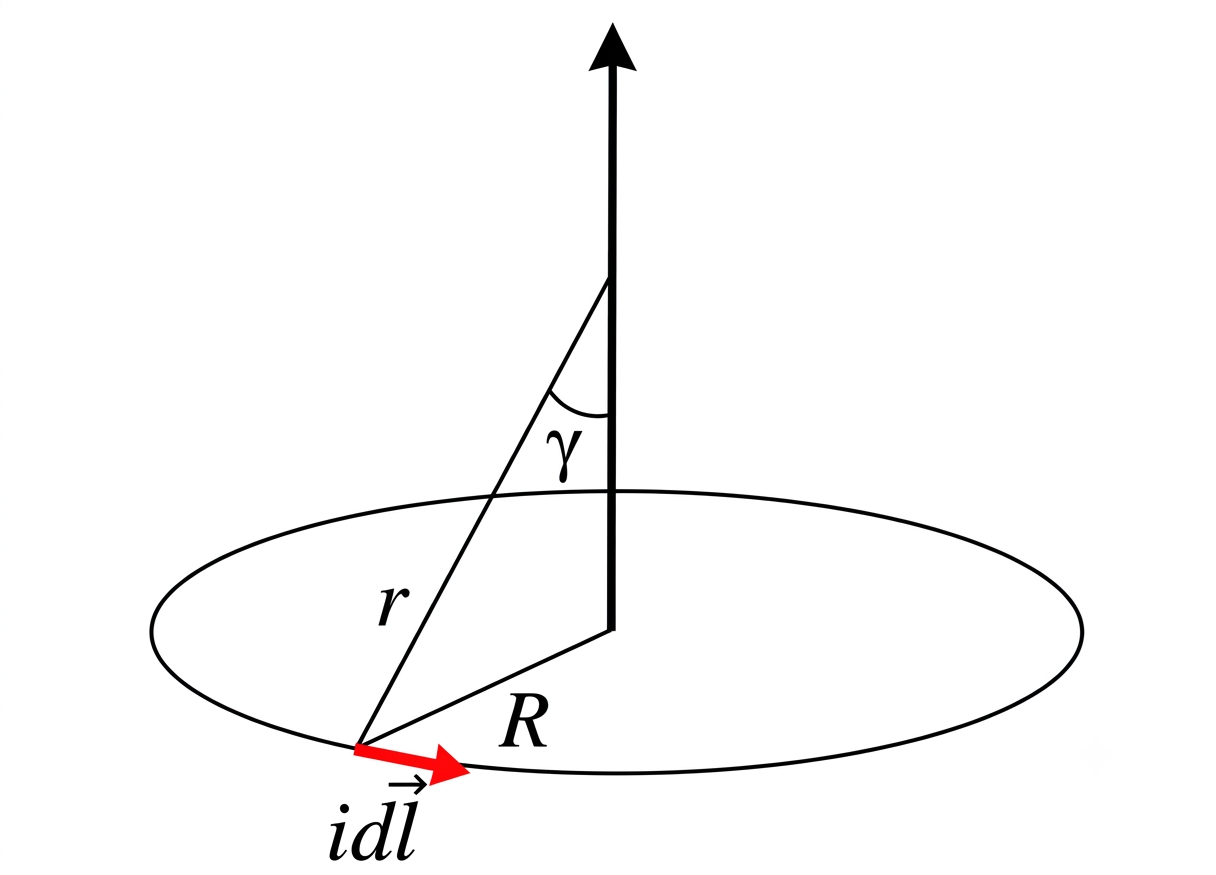
\includegraphics[width=0.4\textwidth]{Fig12}
		\captionof{figure}{\textit{ Magnetic field produced on the axis of a current-carrying coil. }}
	\end{center}
	
	\noindent
	A solenoid consists of a helical winding of wire on a cylinder, usually circular in cross section. There can be hundreds or thousands of closely spaced turns, each of which can be regarded as a circular loop (Fig.2a). Inside solenoid, the field lines are considered to be uniformly spaced as 
	shown in Fig.2b.
	\begin{center}
		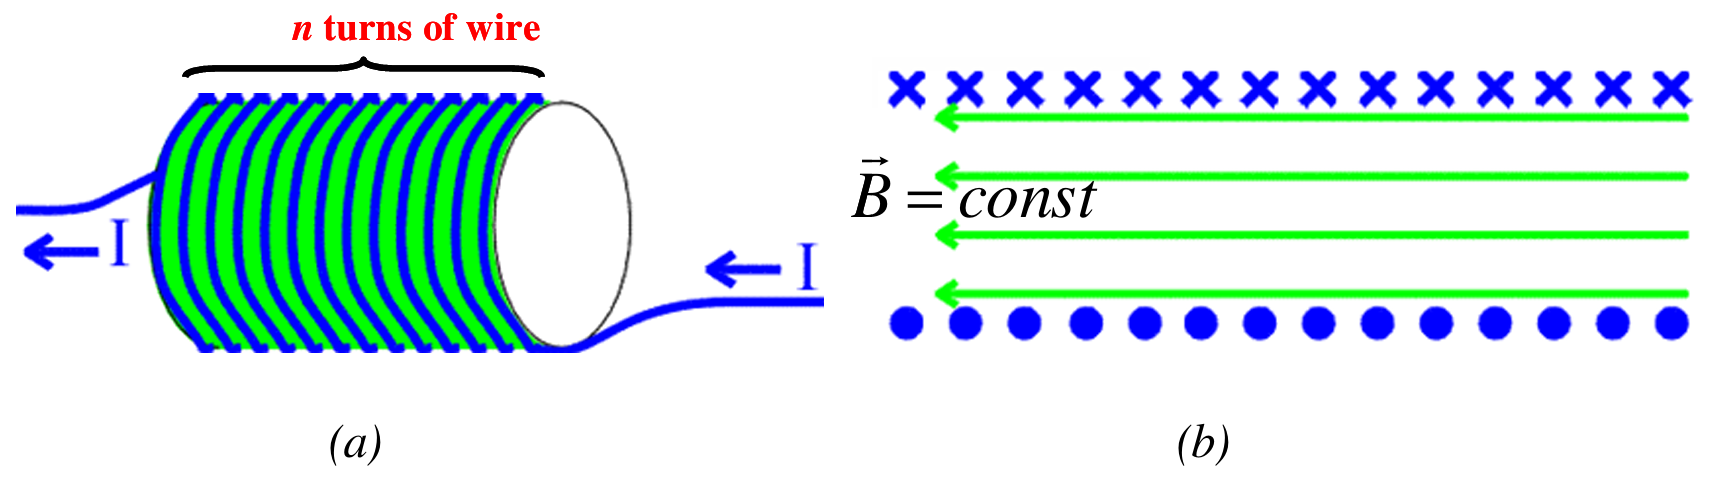
\includegraphics[width=0.85\textwidth]{Fig22}
		\captionof{figure}{\textit{ Typical solenoid (a) and magnetic field lines produced by the currents in it (b)  }}
	\end{center}
	\noindent
	Exact calculations for a long, closely wound solenoid, half of these field lines emerge from the ends and half "leak out" through the windings between the center and the ends. Because all turns carry the same current $I$. then, the total $B$ field at every point is the vector sum of the fields caused by the individual turns. For a unit of length of solenoid $ds$ with $n$ turns (Fig.3), we have
	\begin{equation}
		dB = \dfrac{\mu_0 \mu_r}{2}\dfrac{R^2}{r^3}\cdot I \cdot n \cdot ds
	\end{equation}
	\noindent
	Let point A in Fig. 3 be the reference point, with the positive direction chosen from left to right. It can be seen that $s = -R\cdot \cot \gamma$ $\left(\text{or }ds = R \cdot \dfrac{d\gamma}{\sin^2 \gamma}\right)$, and $\sin \gamma = \dfrac{R}{r}$. Hence, we obtain
	\begin{equation}
		dB = \dfrac{\mu_0 \mu_r}{2}\cdot I \cdot n \cdot \sin \gamma d\gamma
	\end{equation}
	\begin{center}
		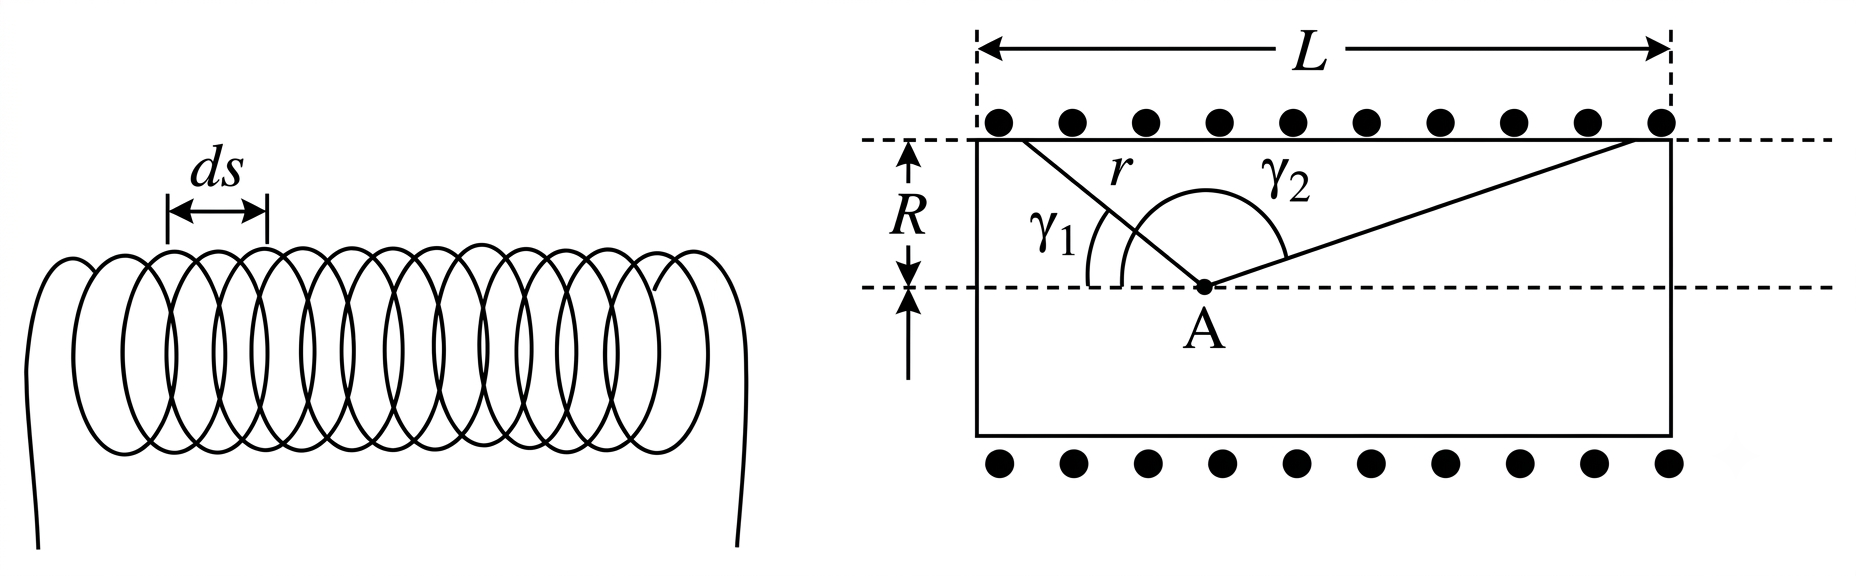
\includegraphics[width=0.85\textwidth]{Fig32}
		\captionof{figure}{\textit{The way to calculate the magnetic field at a point inside a finite solenoid}}
	\end{center}
	
	\noindent
	Using Ampere's law, the magnetic field B produced by a finite solenoid with length L at A as shown in Fig.3 would be
	\begin{equation}
		B = \frac{\mu_0\mu_r}{2} \cdot I \cdot n_0 \int\limits_{\gamma_1}^{\gamma_2} \sin\gamma \, d\gamma = \frac{\mu_0\mu_r}{2} \cdot I \cdot n_0 (\cos\gamma_1 - \cos\gamma_2)
	\end{equation}
	\noindent
	where $n_0 = \dfrac{n}{L}$ is the number of turns per unit length, if the solenoid has $n$ wire turns.
	
	\noindent
	For an infinitely long solenoid ($\gamma_1 = 0$, $\gamma_2 = \pi$), the magnetic field becomes:
	\begin{equation}
		B = \mu_0 \mu_r I n_0
	\end{equation}
	\noindent
	It can be seen that magnetic field produced by a finite coil is smaller than that by an infinite one. Clearly, the magnetic field inside is homogeneous and its strength does not depend on the distance from the axis. This last result, which holds strictly true only near the centre of the solenoid where the field lines are parallel to its length, is the most important.
	
	\section*{3. Experimental procedure}
	
	\subsection*{3.1. Preparation of Measurement}
	Using wires to connect the solenoid, rheostat and ammeter together in series circuit as 
	shown in Fig. 4. In this circumstance, the current provided by an AC power supply, flows 
	through the rheostat then the solenoid. The rheostat is used to monitor the magnitude of current, which is read out with an ammeter. The axial magnetic-induction probe inside solenoid 
	measures the component of the magnetic field along the solenoid symmetry axis. The axial 
	probe can be moved easily along the solenoid. The position of the probe is determined using a 
	linear rule attached with the probe. The magnetic field is read out by the Teslameter. Check if the axial probe had connected with Teslameter. 
	\begin{center}
		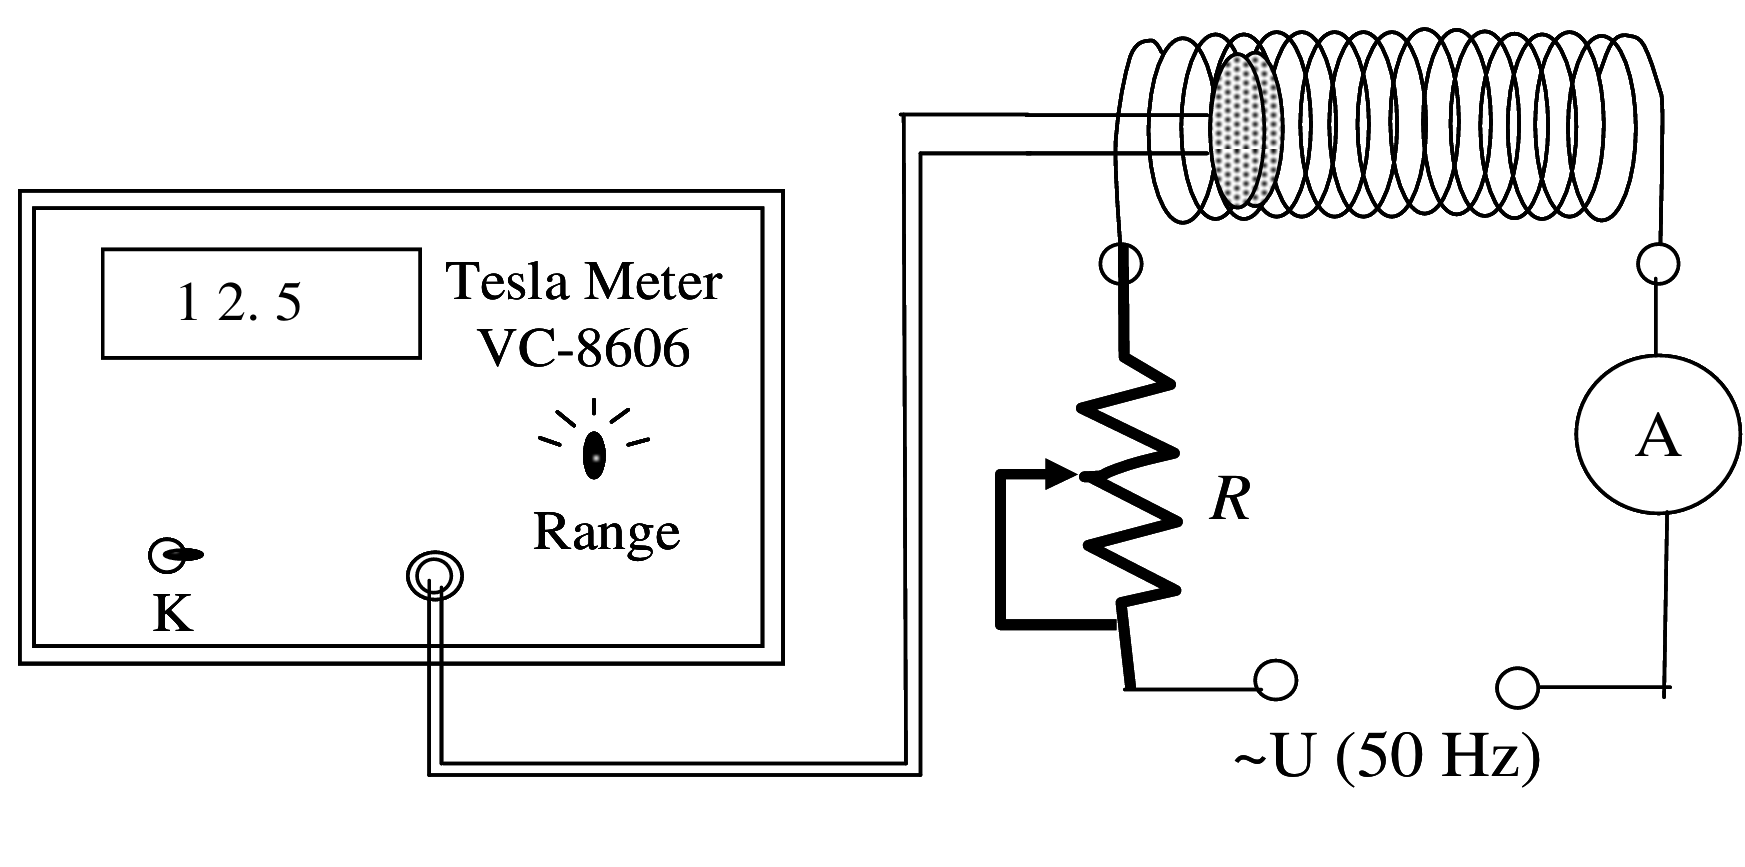
\includegraphics[width=0.5\textwidth]{Fig42}
		\captionof{figure}{\textit{Layout of measurement circuit}}
	\end{center}
	
	
	\subsection*{3.2. Measurement Sequence}
	\subsubsection*{3.2.1. Investigation of magnetic field along the axis - $B(x)$}
	\begin{enumerate}[leftmargin=1.5em]
		\item Place the axial probe so that one end of the solenoid corresponds to position $0$ on the linear rule. Set the power supply voltage to $3\,\text{V}$, turn on the power supply and Teslameter, and record the initial current and magnetic field $B(0)$.
		\item Slowly pull out the probe in increments of $1\,\text{cm}$ up to $30\,\text{cm}$, recording the magnetic field $B(x)$ at each position in Table 1.
	\end{enumerate}
	
	\subsubsection*{3.2.2. Relationship between magnetic field and current - $B(I)$}
	\begin{enumerate}[leftmargin=1.5em]
		\item Fix the axial probe at the center of the coil ($x = 15\,\text{cm}$).
		\item Set the power supply output voltage to $3\,\text{V}$, $6\,\text{V}$, $9\,\text{V}$, and $12\,\text{V}$ successively, recording the current and magnetic field $B(x)$ in Table 2.
	\end{enumerate}
	
	\subsubsection*{3.2.3. Comparison of experimental and theoretical magnetic field}
	\begin{enumerate}[leftmargin=1.5em]
		\item Adjust the rheostat so the ammeter reads $0.4\,\text{A}$ and keep it fixed.
		\item Measure the magnetic field at positions $x = 0\,\text{cm}$, $15\,\text{cm}$, and $30\,\text{cm}$, recording the results in Table 3.
	\end{enumerate}
	
	\section*{4. Experimental results}
	
	\subsection*{4.1. Investigation of the magnetic field at the positions along the axis of solenoid}
	
	\begin{table}[H]
		\centering
		\caption{Measurement of magnetic field $B(x)$ along the solenoid axis with $I = 0.19\text{A}$}
		\begin{tabular}{|>{\centering\arraybackslash}m{1.5cm}|>{\centering\arraybackslash}m{3.5cm}|>{\centering\arraybackslash}m{1.5cm}|>{\centering\arraybackslash}m{3.5cm}|}
			\hline
			\textbf{$x$ (cm)} & \textbf{$B(x)$ (mT)} & \textbf{$x$ (cm)} & \textbf{$B(x)$ (mT)} \rule[-0.2cm]{0pt}{0.6cm} \\
			\hline
			0 & 0.42 & 16 & 0.89 \rule[-0.25cm]{0pt}{0.7cm} \\ \hline
			1 & 0.65 & 17 & 0.89 \rule[-0.25cm]{0pt}{0.7cm} \\ \hline
			2 & 0.76 & 18 & 0.89 \rule[-0.25cm]{0pt}{0.7cm} \\ \hline
			3 & 0.81 & 19 & 0.88 \rule[-0.25cm]{0pt}{0.7cm} \\ \hline
			4 & 0.84 & 20 & 0.88 \rule[-0.25cm]{0pt}{0.7cm} \\ \hline
			5 & 0.85 & 21 & 0.88 \rule[-0.25cm]{0pt}{0.7cm} \\ \hline
			6 & 0.88 & 22 & 0.88 \rule[-0.25cm]{0pt}{0.7cm} \\ \hline
			7 & 0.88 & 23 & 0.87 \rule[-0.25cm]{0pt}{0.7cm} \\ \hline
			8 & 0.88 & 24 & 0.87 \rule[-0.25cm]{0pt}{0.7cm} \\ \hline
			9 & 0.88 & 25 & 0.86 \rule[-0.25cm]{0pt}{0.7cm} \\ \hline
			10 & 0.88 & 26 & 0.85 \rule[-0.25cm]{0pt}{0.7cm} \\ \hline
			11 & 0.88 & 27 & 0.82 \rule[-0.25cm]{0pt}{0.7cm} \\ \hline
			12 & 0.89 & 28 & 0.77 \rule[-0.25cm]{0pt}{0.7cm} \\ \hline
			13 & 0.89 & 29 & 0.68 \rule[-0.25cm]{0pt}{0.7cm} \\ \hline
			14 & 0.89 & 30 & 0.47 \rule[-0.25cm]{0pt}{0.7cm} \\ \hline
			15 & 0.89 & & \rule[-0.25cm]{0pt}{0.7cm} \\ \hline
		\end{tabular}
	\end{table}
	\begin{figure}[H]
		\centering
		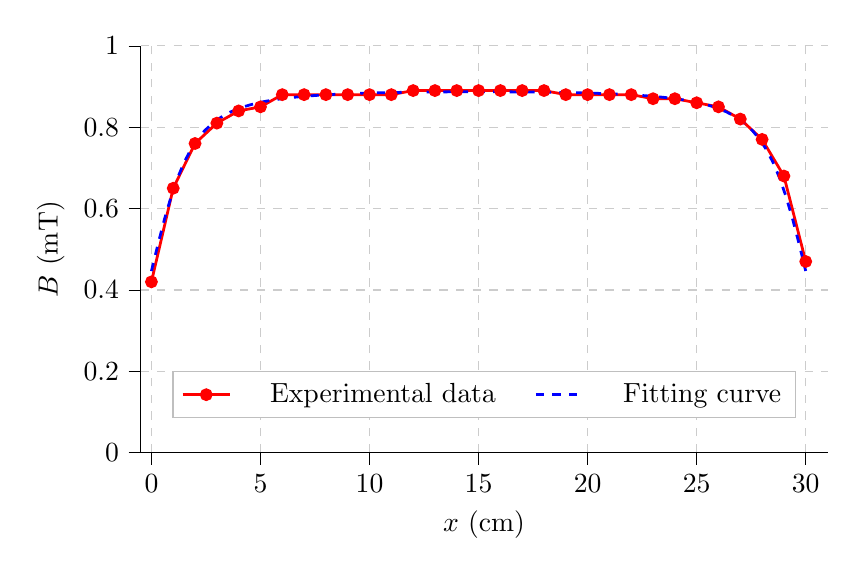
\begin{tikzpicture}
			\begin{axis}[
				width=0.85\textwidth,
				height=6.75cm,
				xlabel={$x$ (cm)},
				ylabel={$B$ (mT)},
				xmin=-0.5, xmax=31,
				ymin=0.0, ymax=1.0,
				xtick={0,5,10,15,20,25,30},
				ytick={0.0,0.2,0.4,0.6,0.8,1.0},
				yticklabel style={/pgf/number format/fixed, /pgf/number format/precision=1},
				grid=major,
				grid style={dashed, gray!40},
				axis lines=left,
				axis line style={-},
				tick align=outside,
				tick style={black},
				legend columns=-1,
				legend style={
					at={(0.5,0.2)},
					anchor=north,
					column sep=12pt,
					draw=gray!50,
				},
				]
				\addplot[
				color=red,
				line width=1pt,
				mark=*,
				mark size=1.8pt,
				] coordinates {
					(0, 0.42)  (1, 0.65)  (2, 0.76)  (3, 0.81)  (4, 0.84)  (5, 0.85)
					(6, 0.88)  (7, 0.88)  (8, 0.88)  (9, 0.88)  (10, 0.88) (11, 0.88)
					(12, 0.89) (13, 0.89) (14, 0.89) (15, 0.89) (16, 0.89) (17, 0.89)
					(18, 0.89) (19, 0.88) (20, 0.88) (21, 0.88) (22, 0.88) (23, 0.87)
					(24, 0.87) (25, 0.86) (26, 0.85) (27, 0.82) (28, 0.77) (29, 0.68)
					(30, 0.47)
				};
				\addplot[
				color=blue,
				dashed,
				line width=1pt,
				domain=0:30,
				samples=100,
				] {0.895 * 0.5 * (x/sqrt(2.015^2 + x^2) + (30 - x)/sqrt(2.015^2 + (30 - x)^2))};
				\addlegendentry{Experimental data}
				\addlegendentry{Fitting curve}
			\end{axis}
		\end{tikzpicture}
		\caption{Distribution of magnetic field $B(x)$ along the solenoid axis}
	\end{figure}
	
	\subsection*{4.2. Measurement of the relationship between the magnetic field and the current through the solenoid}
	\begin{table}[H]
		\centering
		\caption{Measurement of magnetic field $B$ versus voltage $U$ and current $I$}
		\begin{tabular}{|>{\centering\arraybackslash}m{2.5cm}|>{\centering\arraybackslash}m{3.5cm}|>{\centering\arraybackslash}m{4.5cm}|}
			\hline
			\textbf{Trial} & \textbf{Current $I$ (A)} & \textbf{Magnetic Field $B$ (mT)} \rule[-0.2cm]{0pt}{0.6cm} \\
			\hline
			1 & 0.1 & 0.53 \rule[-0.25cm]{0pt}{0.7cm} \\ \hline
			2 & 0.2 & 0.93 \rule[-0.25cm]{0pt}{0.7cm} \\ \hline
			3 & 0.3 & 1.34 \rule[-0.25cm]{0pt}{0.7cm} \\ \hline
			4 & 0.4 & 1.75 \rule[-0.25cm]{0pt}{0.7cm} \\ \hline
			5 & 0.5 & 2.21 \rule[-0.25cm]{0pt}{0.7cm} \\ \hline
			6 & 0.6 & 2.65 \rule[-0.25cm]{0pt}{0.7cm} \\ \hline
		\end{tabular}
	\end{table}
	\begin{figure}[H]
		\centering
		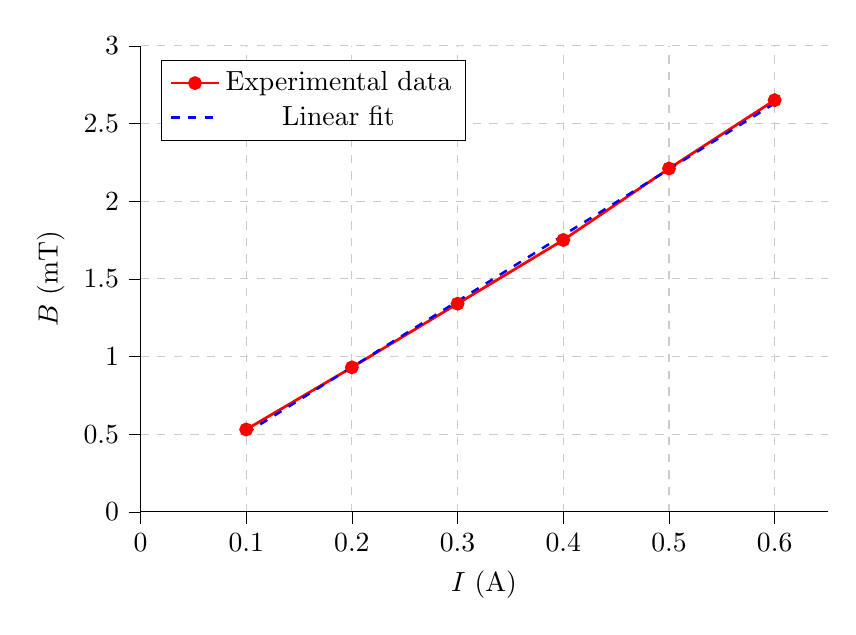
\begin{tikzpicture}
			\begin{axis}[
				width=0.85\textwidth,
				height=7.5cm,
				xlabel={$I$ (A)},
				ylabel={$B$ (mT)},
				xmin=0.0, xmax=0.65,
				ymin=0.0, ymax=3.0,
				xtick={0.0,0.1,0.2,0.3,0.4,0.5,0.6},
				ytick={0.0,0.5,1.0,1.5,2.0,2.5,3.0},
				xticklabel style={/pgf/number format/fixed, /pgf/number format/precision=1},
				yticklabel style={/pgf/number format/fixed, /pgf/number format/precision=1},
				grid=major,
				grid style={dashed, gray!40},
				axis lines=left,
				axis line style={-},
				tick align=outside,
				tick style={black},
				legend pos=north west,
				]
				% Dữ liệu thực nghiệm
				\addplot[
				color=red,
				line width=1pt,
				mark=*,
				mark size=2pt,
				] coordinates {
					(0.1, 0.53)
					(0.2, 0.93)
					(0.3, 1.34)
					(0.4, 1.75)
					(0.5, 2.21)
					(0.6, 2.65)
				};
				\addlegendentry{Experimental data}
				
				% Đường fit tuyến tính (tùy chọn - xóa 4 dòng dưới nếu chỉ muốn vẽ đường nối điểm đo)
				\addplot[
				color=blue,
				dashed,
				line width=0.9pt,
				domain=0.1:0.6,
				] {4.2457*x + 0.0823};
				\addlegendentry{Linear fit}
			\end{axis}
		\end{tikzpicture}
		\caption{Dependence of magnetic field $B$ on current $I$}
	\end{figure}
	
	\subsection*{4.3. Comparison of experimental and theoretical magnetic field }
	
	\noindent
	Two angles $\gamma_1, \gamma_2$ from Eq.(4) are determined by
	\begin{center}
		\vspace{-0.8cm}
		\begin{displaymath}
			\begin{aligned}
				&\cos \gamma_1 = \dfrac{x}{\sqrt{R^2 + x^2}} \\
				&\cos \gamma_2 = \dfrac{-\left(L - x\right)}{\sqrt{R^2 + (L - x)^2}} 
			\end{aligned}
		\end{displaymath}
	\end{center}
	Since an alternating current (AC) source is used, the ammeter measures the root-mean-square current $I = 0.4\text{ A}$, whereas the teslameter records the peak magnetic field amplitude $B_0$. Therefore, the peak current $I_0 = I\sqrt{2}$ is substituted into Eq.(4) to evaluate the theoretical peak magnetic field
	\begin{equation*}
		B_{\text{theo}} = \frac{\mu_0 \mu_r I_0 n_0}{2} (\cos\gamma_1 - \cos\gamma_2) = \frac{\mu_0 \mu_r I\sqrt{2}\, n_0}{2} (\cos\gamma_1 - \cos\gamma_2)
	\end{equation*}
	\noindent
	With the solenoid having the number of wire turns $n = 750$, length $L = 300\text{mm} = 30\text{cm}$, diameter of the cross-section $D = 40.3\text{mm}$, $\mu_r = 1$ (since the environment is air), we yield
	\begin{center}
		\fbox{%
			\begin{minipage}{0.8\textwidth}
				\vspace{-0.4cm}
				\centering
				\begin{displaymath}
					\begin{aligned}
						&x = 0\text{ cm} &\implies B_\text{theo} \approx 0.89\text{ mT} \\
						&x = 15\text{ cm} &\implies B_\text{theo} \approx 1.76\text{ mT} \\
						&x = 30\text{ cm} &\implies B_\text{theo} \approx 0.89\text{ mT}
					\end{aligned}
				\end{displaymath}
			\end{minipage}%
		}
	\end{center}
	\begin{table}[H]
		\centering
		\caption{Comparison of experimental and theoretical magnetic field at $I = 0.4\,\text{A}$}
		\begin{tabular}{|>{\centering\arraybackslash}m{2.5cm}|>{\centering\arraybackslash}m{3.5cm}|>{\centering\arraybackslash}m{3.5cm}|>{\centering\arraybackslash}m{3cm}|}
			\hline
			\textbf{Position $x$ (cm)} & \textbf{$B_{\text{exp}}$ (mT)} & \textbf{$B_{\text{theo}}$ (mT)} & \textbf{Relative Error (\%)} \rule[-0.2cm]{0pt}{0.6cm} \\
			\hline
			0  & 0.85 & 0.89 & 4.13 \rule[-0.25cm]{0pt}{0.7cm} \\ \hline
			15 & 1.75 & 1.76 & 0.64 \rule[-0.25cm]{0pt}{0.7cm} \\ \hline
			30 & 0.92 & 0.89 & 3.77 \rule[-0.25cm]{0pt}{0.7cm} \\ \hline
		\end{tabular}
	\end{table}
	
	\noindent
	From Table 3, we can conclude that the measured magnetic field magnitudes are in close agreement with the theoretical values, as evidenced by the small relative errors. Minor discrepancies arise from measurement uncertainties during data collection.
	

%% =====================================================================
%% EXPERIMENT 3  (content copied unchanged from Ex3-prefinal.tex)
%% =====================================================================
\StartExperiment{3}{Inductor and Free Oscillations in RLC Circuit}
	\renewcommand{\figurename}{Figure}
	\renewcommand{\tablename}{Table}
	
	\begin{center}
		\textbf{\Large EXPERIMENT 3}
		
		\vspace{0.5cm}
		\textbf{{\Large INDUCTOR AND FREE OSCILLATIONS}}
		
		\vspace{0.25cm}
		\textbf{{\Large IN RLC CIRCUIT}}
	\end{center}
	
	\section*{1.  Devices and Purpose of the experiment}
	\begin{center}
		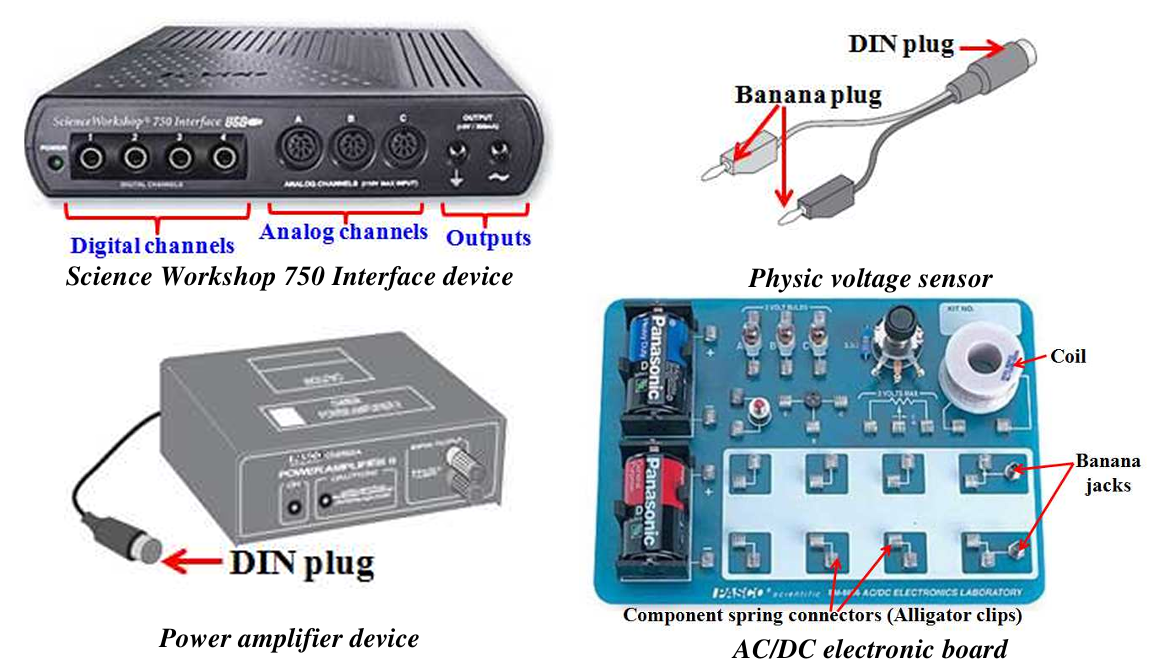
\includegraphics[width=0.9\textwidth]{Devices3}
	\end{center}
	
	\noindent
	The experiment includes two parts. Part 1 is to investigate the current in the RL circuit and 
	consequently to determine the resistance and inductance of a coil with/without a core. Part 2 is to 
	investigate the current and subsequently its frequency as well as the dissipated energy in the 
	RLC circuit.
	
	\section*{2. Theoretical background}
	
	\subsection*{2.1. Inductor and RL circuit}
	An inductor is a 2-terminal circuit element that stores energy in its magnetic field. If a current $i(t)$ is flowing through an inductor, the voltage $V_L$ across the inductor is proportional to the time rate of change of $i$:
	\begin{equation}
		V_L = L \frac{di(t)}{dt}
	\end{equation}
	where $L$ is the inductance in Henry (H).
	When a wound coil is connected with a voltage source $V_S$, we can consider it a series RL circuit. Applying Kirchhoff's voltage law:
	\begin{equation}
		V_S = V_L + V_R = L \frac{di(t)}{dt} + i(t) R = 0
	\end{equation}
	When the voltage source is replaced with a short-circuit, the current in the circuit decays exponentially with time constant $\tau = \frac{L}{R}$:
	\begin{equation}
		i(t) = I_0 e^{-\frac{t}{\tau}}
	\end{equation}
	where $I_0 = \frac{V_S}{R}$ is the current through the circuit at time $t=0$, and $R$ is the pure resistance of the coil:
	\begin{equation}
		R = \frac{V_S}{I_0}
	\end{equation}
	Taking the natural logarithm of both sides of Eq. (3):
	\begin{equation}
		\ln i(t) = -\frac{R}{L}t + \ln I_0
	\end{equation}
	Eq. (5) is a linear function of time $t$ of which the graph has the slope $S = -\frac{R}{L}$. Therefore, the inductance $L$ can be calculated as:
	\begin{equation}
		L = \frac{R}{|S|} = \frac{V_S}{I_0 \cdot |S|}
	\end{equation}
	\begin{center}
		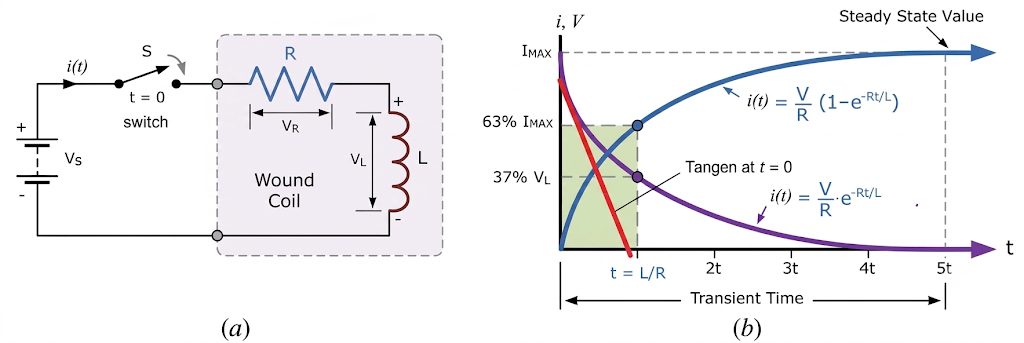
\includegraphics[width= \textwidth]{Log Graph}
		\captionof{figure}{\textit{Principal RL circuit (a) and currents flow through the circuit (b)}}
	\end{center}
	
	\subsection*{2.2. Oscillation in RLC circuit}
	For a series LC circuit where the internal resistance of the inductor is non-negligible, it can be considered an RLC circuit. The differential equation without any external voltage is:
	\begin{equation}
		L \frac{d^2 i}{dt^2} + R \frac{di}{dt} + \frac{i}{C} = 0
	\end{equation}
	The solution of Eq. (7) is:
	\begin{equation}
		i(t) = I_0 e^{-\gamma t} \cos(\omega t)
	\end{equation}
	where the exponential decay coefficient $\gamma = \frac{R}{2L}$, and the natural angular frequency of the LC oscillator is $\omega^2 = \frac{1}{LC}$ $\left( \text{or we can say } \omega = \dfrac{1}{\sqrt{LC}} \right)$.
	\begin{center}
		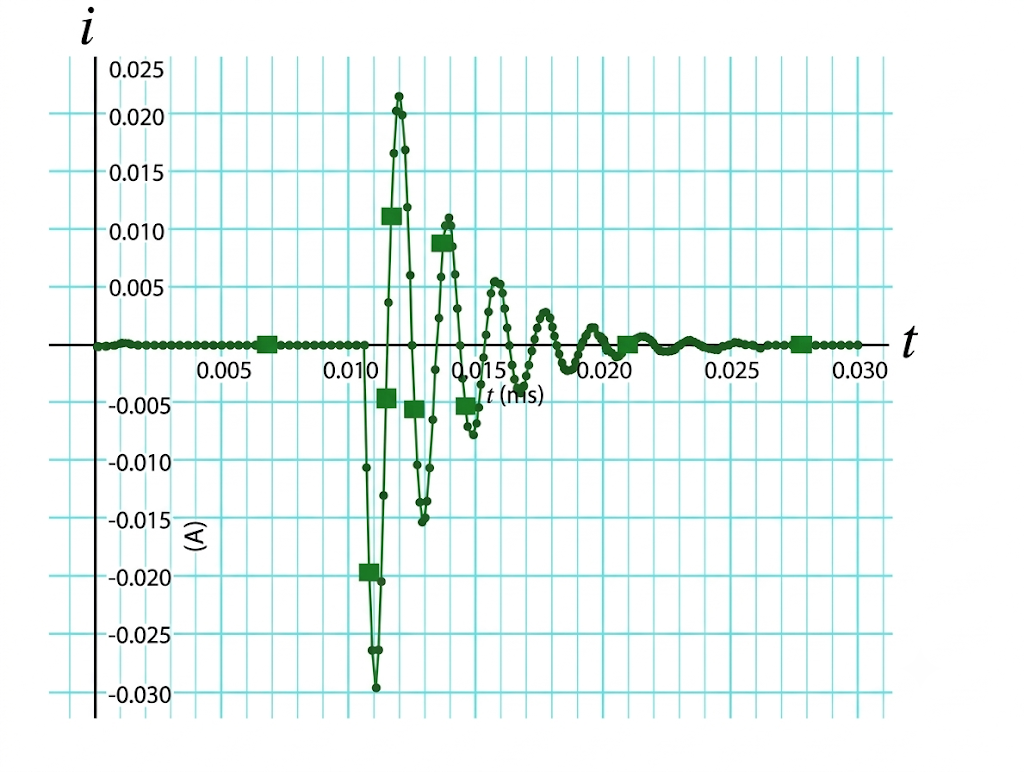
\includegraphics[width= 0.6\textwidth]{RLC circuit graph}
		\captionof{figure}{\textit{Current in a RLC circuit}}
	\end{center}
	
	\subsection*{2.3. Energy in RLC circuit}
	\begin{minipage}[t]{0.48\textwidth}
		\noindent
		The energy stored in the magnetic field of the inductor is:
		\begin{equation}
			U_B = \frac{1}{2} L i^2
		\end{equation}
		and in the electric field of the capacitor is:
		\begin{equation}
			U_E = \frac{1}{2} C V^2
		\end{equation}
		The total energy stored in the electric and magnetic fields is:
		\begin{equation}
			U = U_B + U_E = \frac{1}{2} L i^2 + \frac{1}{2} C V^2
		\end{equation}
		This energy is gradually being lost as heat in the resistor at the rate $I^2 R$ (Joule heating).
	\end{minipage}%
	\hfill%
	\begin{minipage}[t]{0.48\textwidth}
		\centering
		\raisebox{-\height}{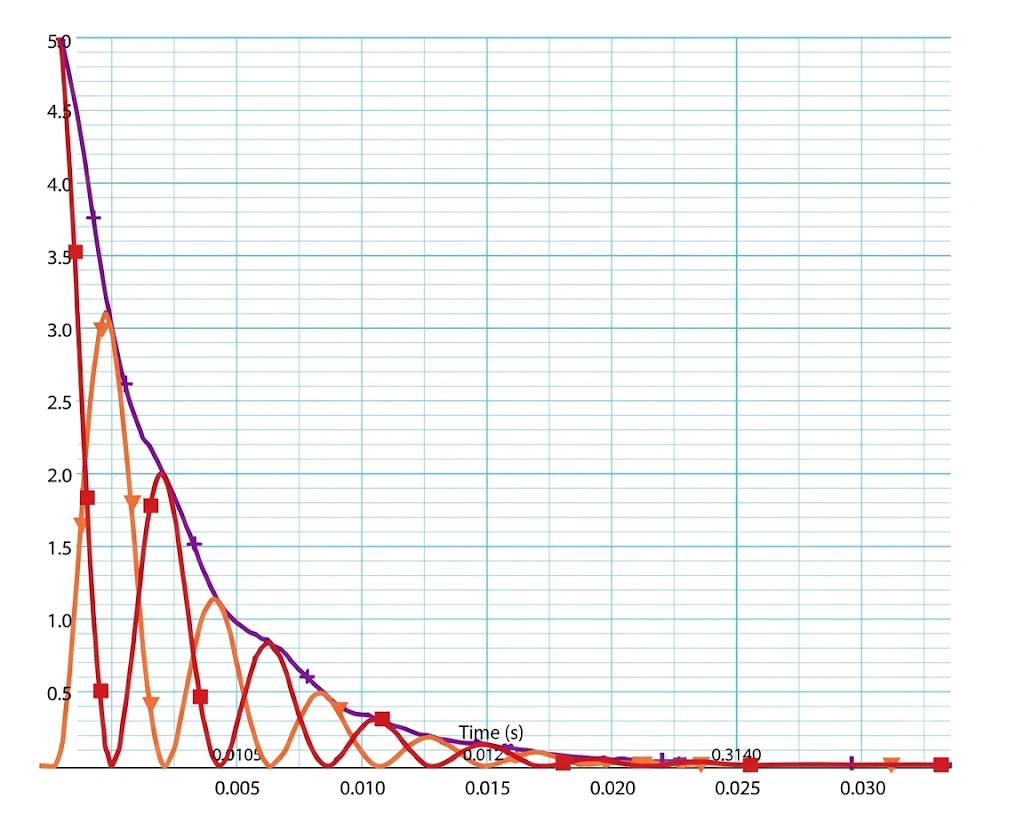
\includegraphics[width= \textwidth]{Energy in RLC}}
		\captionof{figure}{\textit{Energy in RLC circuit also exponential decays}}
	\end{minipage}
	
	\section*{3. Experimental procedure}
	
	\subsection*{3.1. Current, resistance and inductance in RL circuit}
	\subsubsection*{3.1.1. Preparation for measurement}
	\begin{itemize}[leftmargin=1.5em]
		\item Connect two terminals of the coil to the springs next to the top banana jack. Connect patch cords from "OUTPUT" ports of interface to banana jacks on the board.
		\item Set up Data Studio: Connect Voltage Sensor to Channel A, Power Amplifier to Channel C.
		\item Set Signal Generator: Positive Square Wave, frequency 20 Hz, Amplitude 1 V, Sample rate 10,000 Hz, measurement time 0.5 s.
	\end{itemize}
	
	\subsubsection*{3.1.2. Measurement sequence}
	\begin{enumerate}[leftmargin=1.5em]
		\item Click "Start". Drag $\text{Run}^\#1$ file to "Graph" to display output voltage. Define and record $I_0$. Calculate coil resistance $R$ using $R = \frac{V_S}{I_0}$ with $V_S = 1\text{ V}$.
		\item Click "Calculate", apply $\ln$ function to measurement data according to Eq. (5).
		\item Drag the calculated $\ln i(t)$ result to graph display. Select linear region and perform "Curve Fit / Linear Fit" to obtain the Slope ($S$).
		\item Calculate inductance $L$ using $L = \frac{V_S}{I_0 \cdot S}$.
		\item Insert a metal core inside the coil and repeat Steps 1 to 4 to determine inductance with core.
	\end{enumerate}
	
	\subsection*{3.2. Current and energy in RLC circuit}
	\subsubsection*{3.2.1. Preparation for measurement}
	\begin{itemize}[leftmargin=1.5em]
		\item Connect a $10\,\mu\text{F}$ capacitor in series with the coil. Connect Voltage Sensor across capacitor terminals.
		\item Keep the measurement regime established in Section 2.1.1.
	\end{itemize}
	
	\subsubsection*{3.2.2. Measurement sequence}
	\begin{enumerate}[leftmargin=1.5em]
		\item Click "Start" to record data.
		\item Calculate magnetic energy $U_B = \frac{1}{2} L i^2$ using "pow(x,2)" function with calculated $L$ (without core).
		\item Calculate electric energy $U_E = \frac{1}{2} C V^2$ using $C = 10\,\mu\text{F} = 0.00001\text{ F}$.
		\item Calculate total energy $U = U_B + U_E$.
		\item Display graphs of $U_B$, $U_E$, and total energy $U$.
		\item Save all data to storage.
	\end{enumerate}
	
	\section*{4. Experimental results}
	\subsection*{4.1. Resistance and Inductance of the Coil}
	\hspace{1.23em}
	Initial current $\text{ I}_0 = 0.13 \text{ A}$
	
	\vspace{0.2cm}
	Measured slope (without core) $\text{S}_{\text{w/o}} = -951.50$
	
	\vspace{0.2cm}
	Measured slope (without core) $\text{S}_{\text{w}} = -190.35$
	
	\vspace{0.2cm}
	The resistance of the coil
	\begin{center}
		\fbox{%
			\begin{minipage}{0.8\textwidth}
				\vspace{-0.4cm}
				\centering
				\begin{displaymath}
					R_L = \frac{V_S}{I_0} = \dfrac{1}{0.13} \approx 7.69 \left(\Omega\right)
				\end{displaymath}
			\end{minipage}%
		}
	\end{center}
	
	Coil inductance without core
	\begin{center}
		\fbox{%
			\begin{minipage}{0.8\textwidth}
				\vspace{-0.4cm}
				\centering
				\begin{displaymath}
					L_{\text{w/o}} = \dfrac{V_S}{I_0  \left|\text{S}_{\text{w/o}}\right|} \approx \dfrac{1}{0.13 \times 951.50} \approx 8.10 \times 10^{-3}  \left(\text{H}\right) = 8.10 \left(\text{mH}\right)
				\end{displaymath}
			\end{minipage}%
		}
	\end{center}
	
	Coil inductance with core
	\begin{center}
		\fbox{%
			\begin{minipage}{0.8\textwidth}
				\vspace{-0.4cm}
				\centering
				\begin{displaymath}
					L_{\text{w}} = \dfrac{V_S}{I_0  \left|\text{S}_{\text{w}}\right|} \approx \dfrac{1}{0.13 \times 190.35} \approx 40.41 \times 10^{-3}  \left(\text{H}\right) = 40.41 \left(\text{mH}\right)
				\end{displaymath}
			\end{minipage}%
		}
	\end{center} 
	
	\begin{bt}
		\textit{Briefly explain the difference of inductance of the coil (with/without core)}
	\end{bt}
	After placing an iron core inside the coil, the coil's inductance increases. This phenomenon occurs since iron has a high magnetic permeability compared to air, enhancing the magnetic flux linkage per unit current inside the coil.
	
	\subsection*{4.2. Free Oscillations of the RLC circuit}
	\hspace{1.23em}
	Measured period $\text{ T}_{\text{measured}} = 0.0017 \text{ s}$
	
	\vspace{0.2cm}
	Measured frequency
	\begin{center}
		\fbox{%
			\begin{minipage}{0.8\textwidth}
				\vspace{-0.4cm}
				\centering
				\begin{displaymath}
					\text{f}_{\text{measured}} = \dfrac{1}{\text{T}_{\text{measured}}} = \dfrac{1}{0.0017} \approx 588.24 \left(\text{Hz}\right)
				\end{displaymath}
			\end{minipage}%
		}
	\end{center}
	
	Expected frequency (theoretical frequency)
	\begin{center}
		\fbox{%
			\begin{minipage}{0.8\textwidth}
				\vspace{-0.4cm}
				\centering
				\begin{displaymath}
					\text{f}_{\text{prediction}} = \dfrac{1}{2\pi \sqrt{L_{\text{w/o}} C}} \approx \dfrac{1}{2\pi\sqrt{\left(8.10 \times 10^{-3}\right) \times \left(10 \times 10^{-6}\right)}} \approx 559.21 \left(\text{Hz}\right)
				\end{displaymath}
			\end{minipage}%
		}
	\end{center}
	
	Frequency difference
	\begin{center}
		\fbox{%
			\begin{minipage}{0.8\textwidth}
				\vspace{-0.4cm}
				\centering
				\begin{displaymath}
					\Delta \text{f} = \text{f}_{\text{prediction}} - \text{f}_{\text{measured}} = 559.21 - 588.24 = -29.03 \left(\text{Hz}\right)
				\end{displaymath}
			\end{minipage}%
		}
	\end{center}
	
	\begin{bt}
		\textit{Comments and conclusions on frequency comparison ($\text{f}_{\text{prediction}}$ vs $\text{f}_{\text{measured}}$)}
		
		\vspace{0.2cm}
		The measured frequency ($\text{f}_{\text{measured}} \approx 588.24\text{ Hz}$) is higher than the theoretical prediction ($\text{f}_{\text{prediction}} \approx 559.21\text{ Hz}$), with an absolute difference of $\left|\Delta \text{f}\right| = 29.03\text{ Hz}$.   This discrepancy primarily comes from the non-ideal properties of the circuit components, including the internal resistance and inductance of the connecting wires, as well as the uncertainty in the nominal values of $L$ and $C$. Overall, the measured result shows reasonable agreement with the theoretical model for free RLC oscillations.
	\end{bt}
	
	\begin{bt}
		\textit{Make the comment and discussions of obtained result of energy in RLC circuit. It can be seen that the circuit is losing energy most rapidly at times when the graph of total energy is steepest; these times occur at about the same times that the magnetic energy reaches a local maximum. Briefly explain why.}
		\subsubsection*{1. Comment}
		\hspace{1.23em}
		After the external power source is disconnected, the total energy of the circuit does not drop instantly to zero; instead, it decays gradually. Energy continuously shifts back and forth between the capacitor's electric field and the inductor's magnetic field in a damped cycle, with peak levels decline over time.
		
		\vspace{0.2cm}
		
		\subsubsection*{2. Explanation}
		\hspace{1.23em}
		By the Eq. $(11)$, take derivatives in both sides, notice that $U_E = \dfrac{1}{2} CV^2 = \dfrac{1}{2} \dfrac{q^2}{C}$
		\begin{equation}
			\dfrac{dU}{dt} = \dfrac{dU_B}{dt} + \dfrac{dU_E}{dt} = iL \dfrac{di}{dt} + q\dfrac{dq}{dt} \dfrac{1}{C} = iL \dfrac{di}{dt} + q \dfrac{i}{C} = i\left(L\dfrac{di}{dt} + \dfrac{q}{C}\right)
		\end{equation}
		
		By Kirchoff's law for RLC circuit, we have
		\begin{equation}
			V_L + V_S + V_C = 0 \implies L\dfrac{di}{dt} + iR + \dfrac{q}{C} = 0 \implies -iR = L\dfrac{di}{dt} + \dfrac{q}{C} \implies \dfrac{dU}{dt} = -i^2R
		\end{equation}
		
		Hence, the total energy in a damped RLC circuit decreases over time due to Joule heating across the resistor, with a rate of energy loss given by $\frac{dU}{dt} = -i^2 R$. The circuit loses energy most rapidly when the absolute rate of energy change (the slope of the total energy curve) is at its maximum, which occurs precisely when the magnitude of the current $\vert{}i\vert{}$ reaches its peak. Since the magnetic energy stored in the inductor is expressed as $U_B = \frac{1}{2} L i^2$, these peak current moments correspond directly to the local maxima of the magnetic energy. Consequently, the steepest points on the total energy graph coincide with the times when magnetic energy reaches its local maximum.
	\end{bt}
	

%% =====================================================================
%% EXPERIMENT 4  (content copied unchanged from Ex4-prefinal.tex)
%% =====================================================================
\StartExperiment{4}{Verification of Faraday's Law of Electromagnetic Induction}
	\renewcommand{\figurename}{Figure}
	\renewcommand{\tablename}{Table}
	
	\begin{center}
		\textbf{\Large EXPERIMENT 4}
		
		\vspace{0.5cm}
		\textbf{\Large VERIFICATION OF FARADAY'S LAW OF}
		
		\vspace{0.25cm}
		\textbf{{\Large ELECTROMAGNETIC INDUCTION}}
	\end{center}
	
	\section*{1.  Devices and Purpose of the experiment}
	\begin{center}
		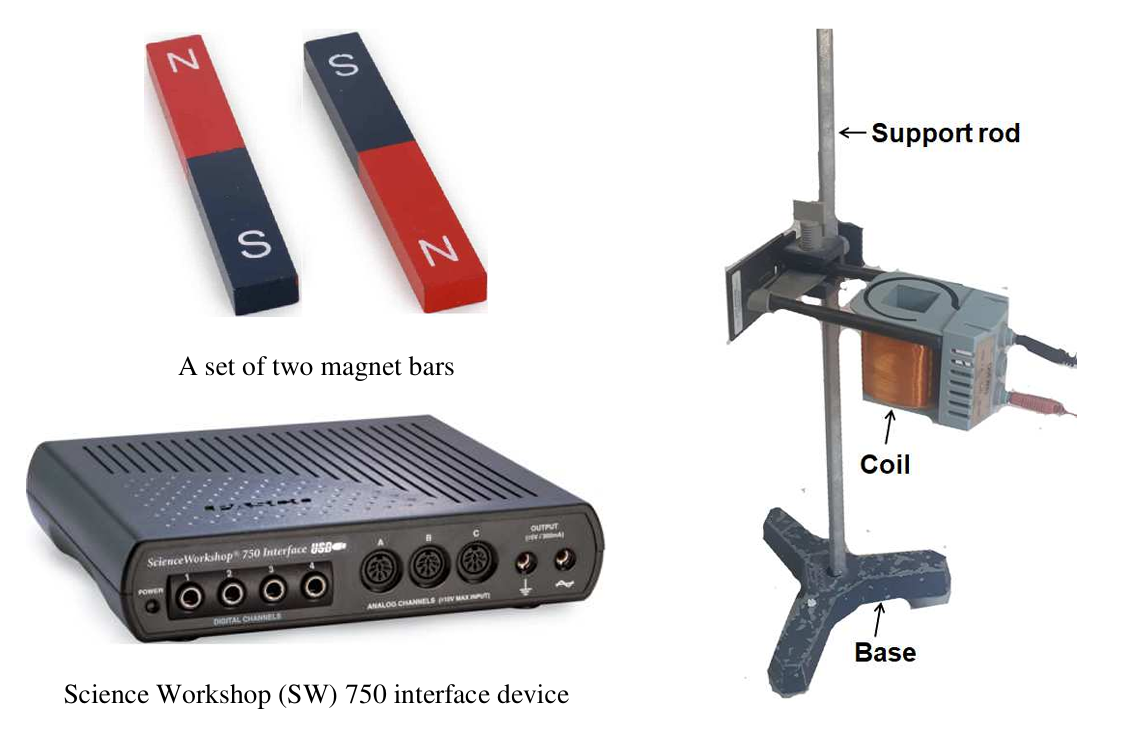
\includegraphics[width=0.8\textwidth]{Devices4}
	\end{center}
	\noindent
	The experiment is to measure the voltage across a coil of wire when a bar magnet moves through it according to Faraday’s law.
	
	\section*{2. Theoretical background}
	\qquad Michael Faraday was the first scientist to find that electricity can be produced from magnetism. He discovered that when a magnet is moving relative to a coil consisting of a number of turns of conductive wire, there will be a voltage across the coil of wire as a result. The essence of his discovery is described in the following statement
	
	\textit{\textbf{A voltage is induced in a circuit whenever relative motion exists between a conductor and a magnetic field, and the magnitude of this voltage is proportional to the rate of change of the flux}}.
	\begin{equation}
		V_{\text{induced}} = -N \frac{\Delta \Phi}{\Delta t} = -N \frac{\Delta(BA)}{\Delta t}
	\end{equation}
	where $N$ is the number of wire's turns, $A$ is the cross-section area of the coil, and $\Delta \Phi$ is the change in magnetic flux resulting from the change in magnetic field $\Delta B$.
	
	Because electricity is induced by a changing magnetic field, this process is called electromagnetic induction. Faraday also realized several factors that determine how much voltage is induced: the strength of the magnetic field, how fast the magnetic field changes, and the number of turns (loops) of wire in the coil.
	
	\section*{3. Experimental procedure}
	
	\subsection*{3.1. Preparation of measurement}
	\begin{itemize}[leftmargin=1.5em]
		\item Turn on the SW 750 interface device and the computer.
		\item Plug a voltage sensor into channel A (or B) of Science Workshop 750 and connect it to the coil terminals.
		\item Launch Data Studio program, drag and drop "Voltage sensor" to channel A, set measurement regime as "Medium" and frequency as 500 Hz.
		\item Place a protective pad or cushion underneath the coil to catch the bar magnet after it falls through.
		\item Prepare two data tables for the 1200-turn and 150-turn coils. Each table has 3 columns: \textit{"Magnet's pole"}, \textit{"Voltage peak 1 (mV)"}, and \textit{"Voltage peak 2 (mV)"}.
	\end{itemize}
	
	\subsection*{3.2. Measurement sequence}
	\subsubsection*{3.2.1. 1200-turn coil}
	\begin{enumerate}[leftmargin=1.5em]
		\item Hold the bar magnet above the 1200-turn coil with the 'North - N' end at the bottom.
		\item Press "Start" on Data Studio interface, release the bar magnet to drop freely through the center of the coil, then press "Stop".
		\item Drag file $\text{Run}^\#1$ to "Graph" to display the induced voltage pulse.
		\item Use the "Point" tool to determine Voltage Peak 1 and Voltage Peak 2. Record values in the table and store the graph.
		\item Reverse the bar magnet so the 'South - S' end falls through first, and repeat the procedure.
		\item Tape two bar magnets together so each end has a combined 'north' and 'south' pole, and repeat the measurement.
		\item Rearrange the two bar magnets so one end is 'north-north' and the other is 'south-south', and repeat the measurement.
	\end{enumerate}
	
	\subsubsection*{3.2.2. 150-turn coil}
	Repeat the measurement procedure similarly for the 150-turn coil using single and double bar magnets, and record results in the second data table.
	
	\section*{4. Experimental results}
	
	\subsection*{4.1. 1200-turn coil}
	\subsubsection*{4.1.1. Graph}
	\begin{center}
		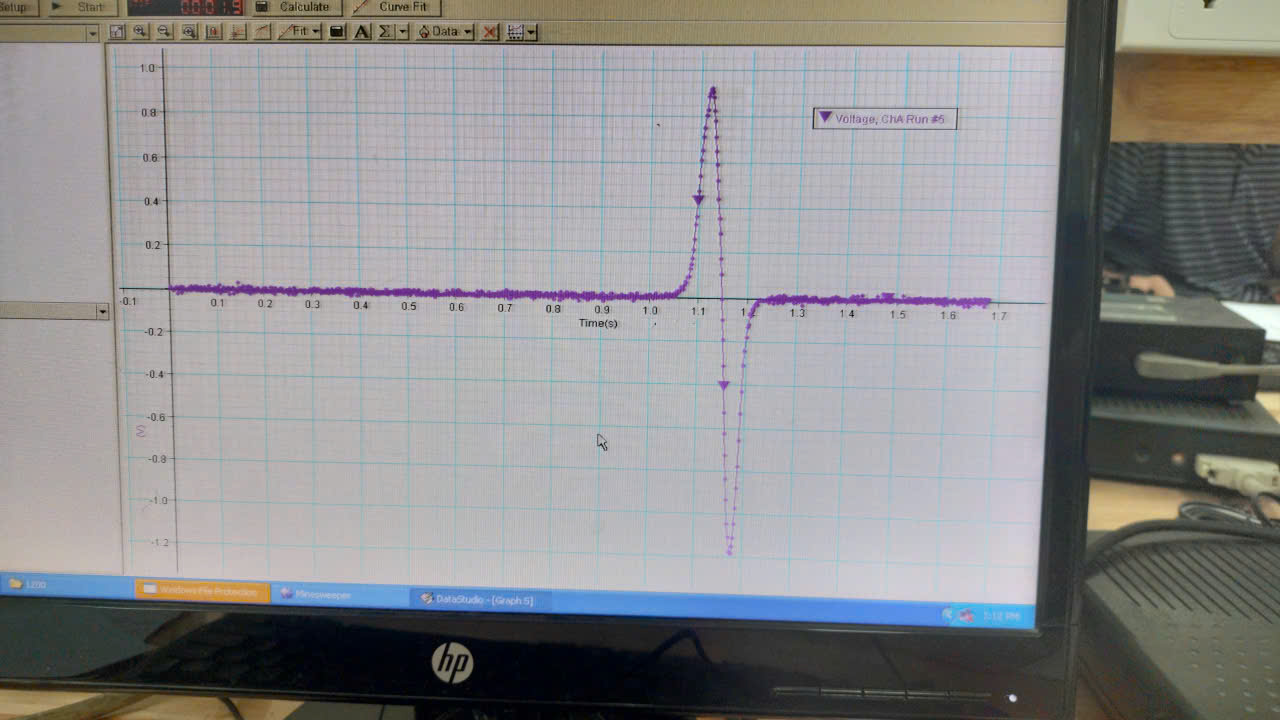
\includegraphics[width=0.95\textwidth]{1200 N.jpg}
		\captionof{figure}{\textit{North-pole down}}
	\end{center}
	
	\begin{center}
		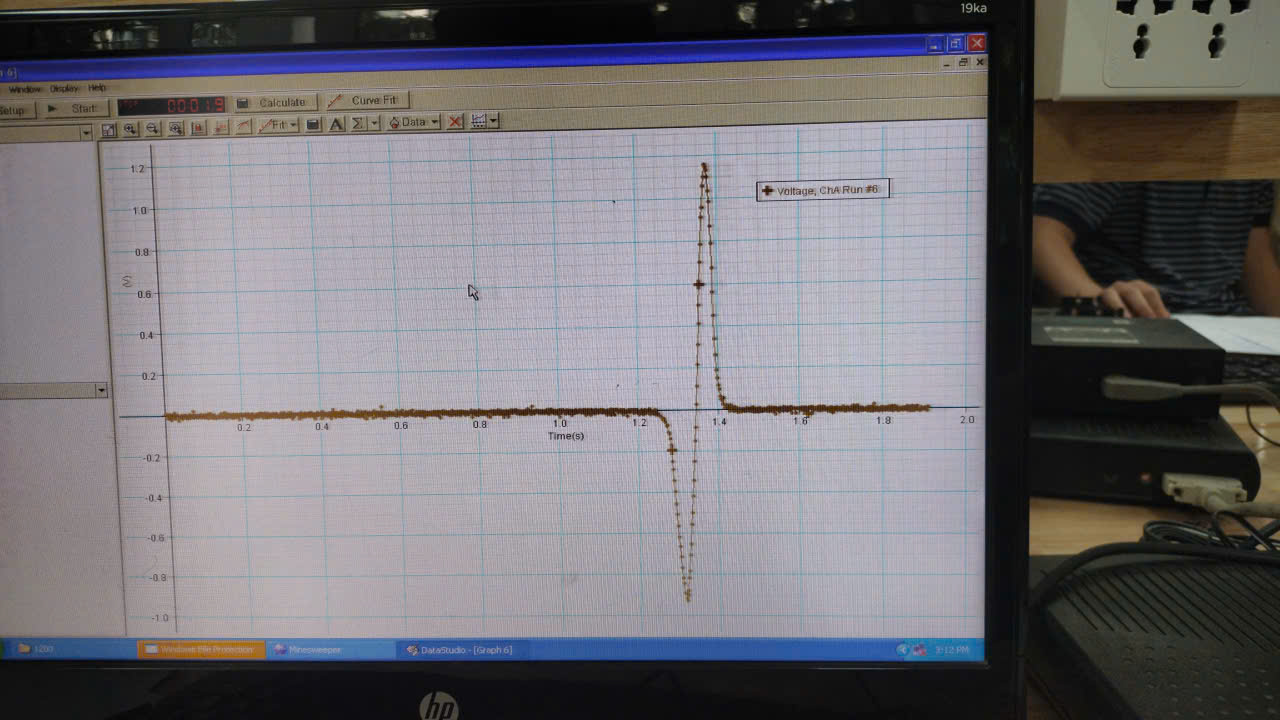
\includegraphics[width=0.95\textwidth]{1200 S.jpg}
		\captionof{figure}{\textit{South-pole down}}
	\end{center}
	
	\begin{center}
		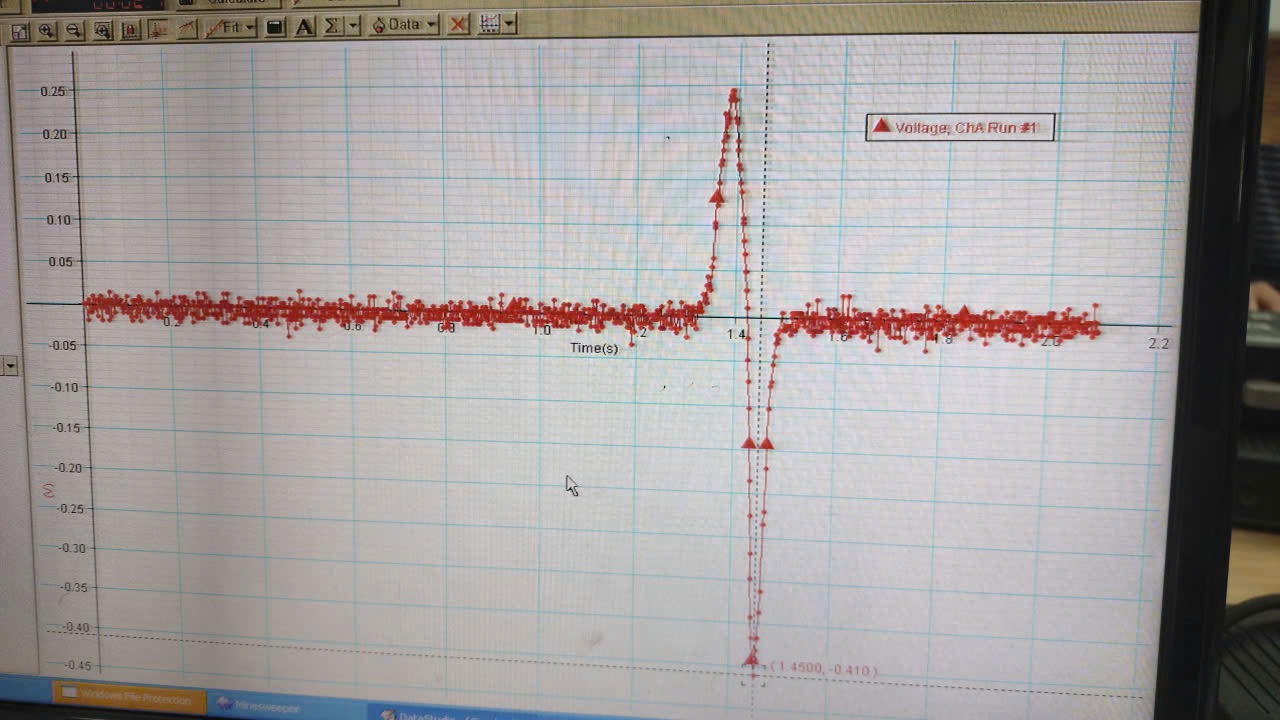
\includegraphics[width=0.95\textwidth]{1200 NS.jpg}
		\captionof{figure}{\textit{North-South combined}}
	\end{center}
	
	\begin{center}
		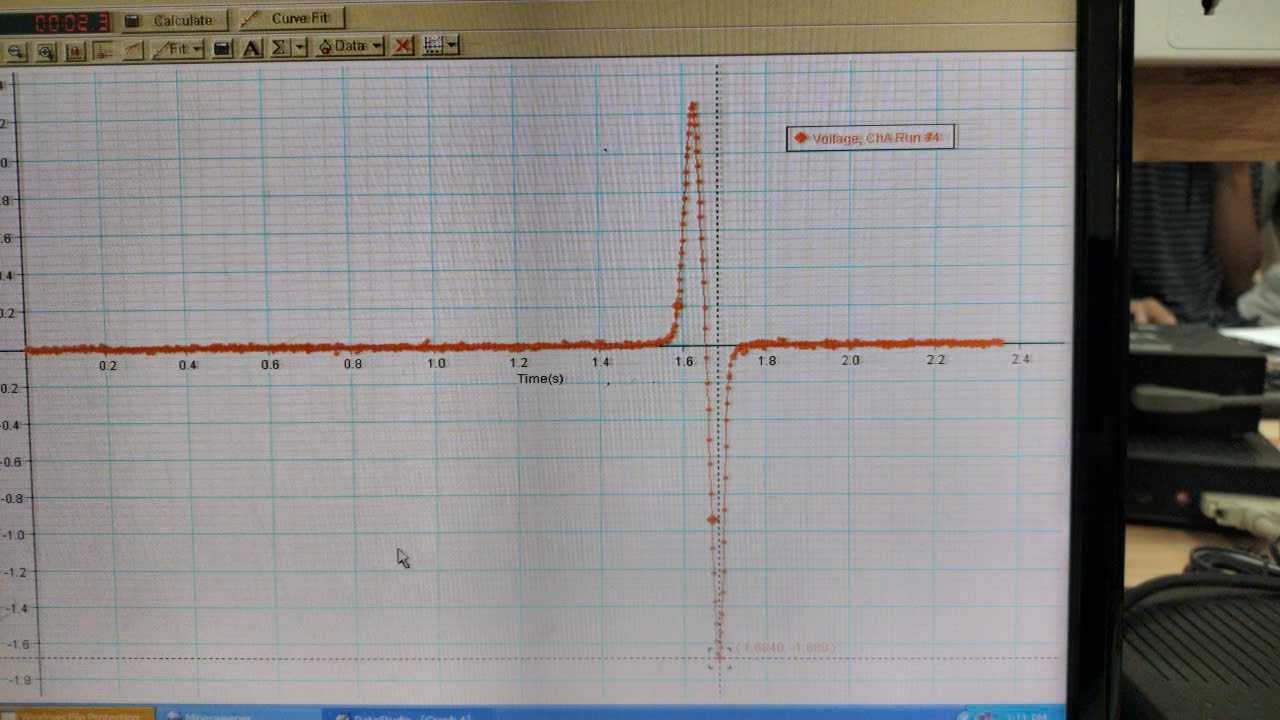
\includegraphics[width=0.95\textwidth]{1200 NN.jpg}
		\captionof{figure}{\textit{North-North down}}
	\end{center}
	
	\subsubsection*{4.1.2. Data Table of Induced Voltage}
	\begin{table}[H]
		\centering
		\caption{Measurement results for 1200-turn coil}
		\begin{tabular}{lccc}
			\toprule
			\textbf{Magnet's pole} & \textbf{Voltage peak 1 (mV)} & \textbf{Voltage peak 2 (mV)} \\
			\midrule
			North pole (N down) & $923$ & $-1187$ \\
			South pole (S down) & $-928$ & $1157$ \\
			Double magnet (N-S combined) & $244$ & $-410$ \\
			Double magnet (N-N / S-S) & $1250$ & $-1680$ \\
			\bottomrule
		\end{tabular}
	\end{table}
	
	\subsection*{4.2. 150-turn coil}
	\subsubsection*{4.2.1. Graph}
	\begin{center}
		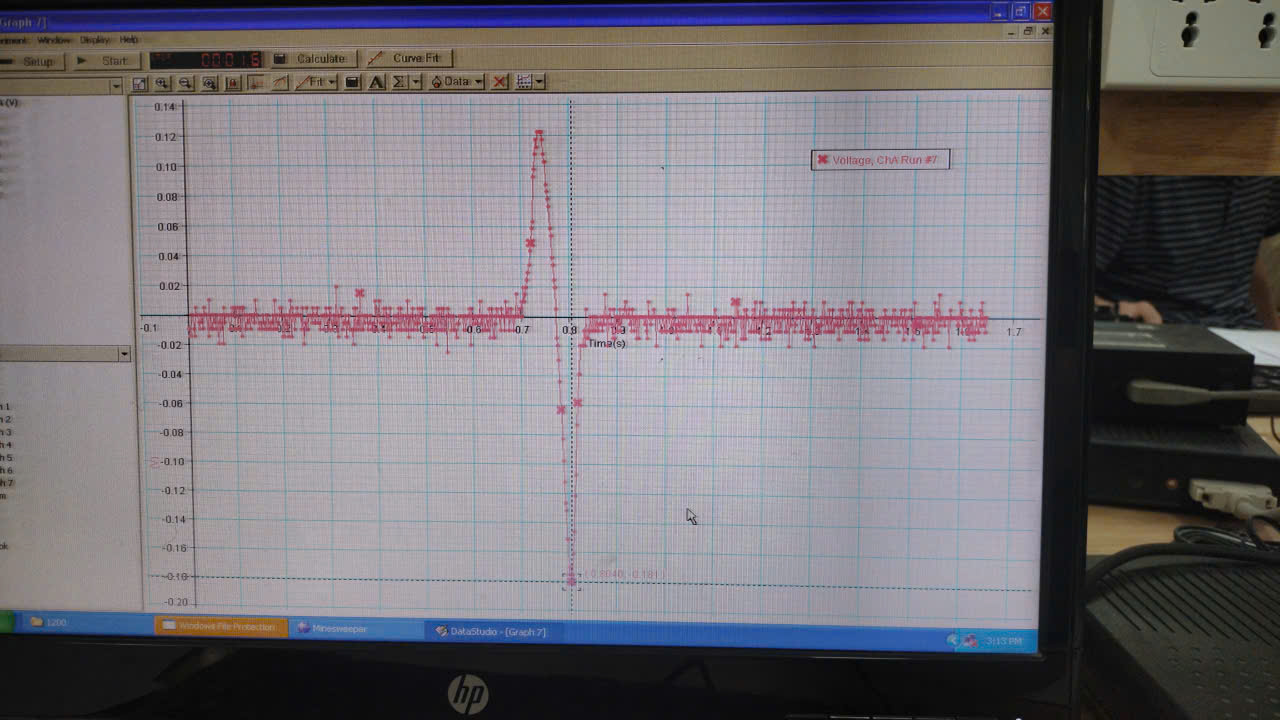
\includegraphics[width=0.95\textwidth]{150 N.jpg}
		\captionof{figure}{\textit{North-pole down}}
	\end{center}
	
	\begin{center}
		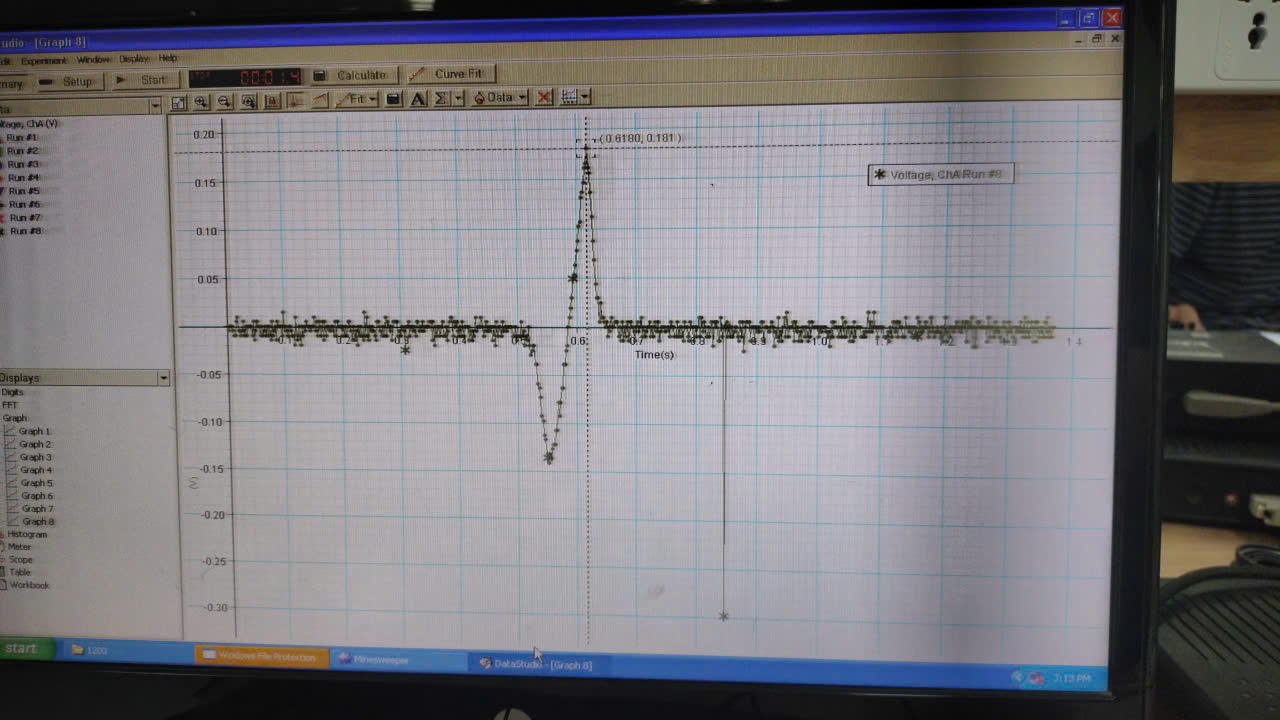
\includegraphics[width=0.95\textwidth]{150 S.jpg}
		\captionof{figure}{\textit{South-pole down}}
	\end{center}
	
	\begin{center}
		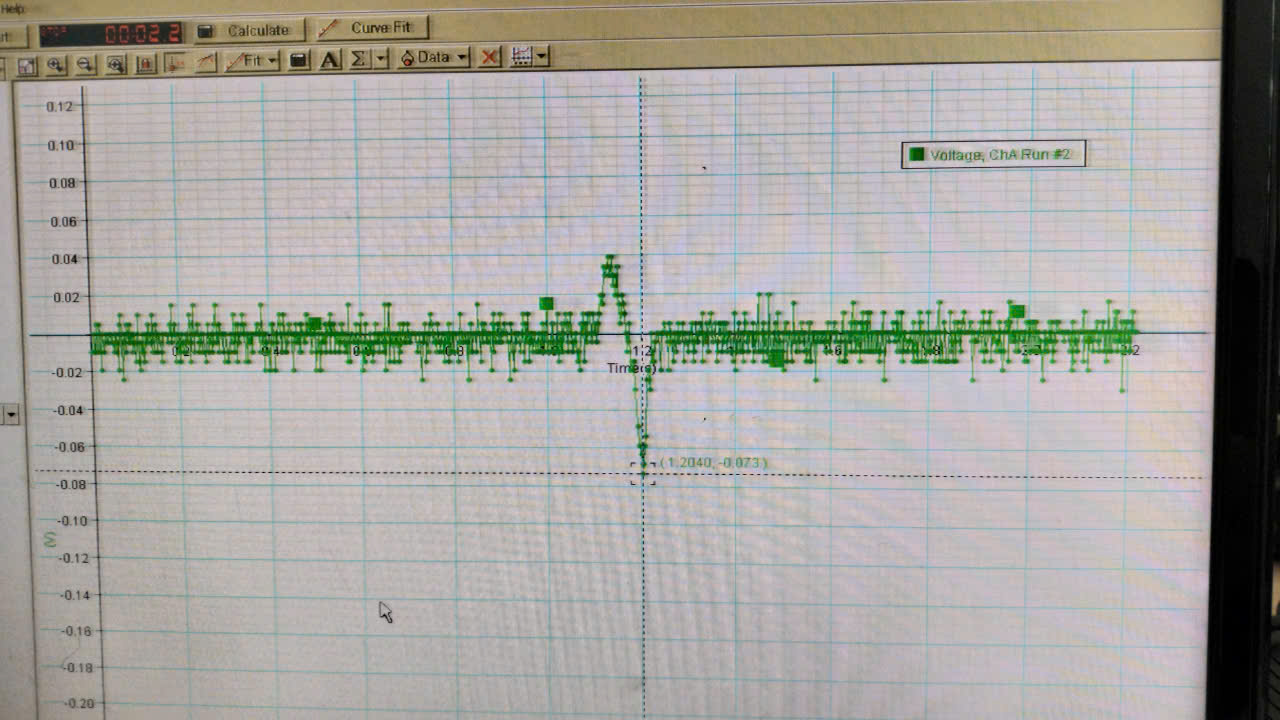
\includegraphics[width=0.95\textwidth]{150 NS.jpg}
		\captionof{figure}{\textit{North-South combined}}
	\end{center}
	
	\begin{center}
		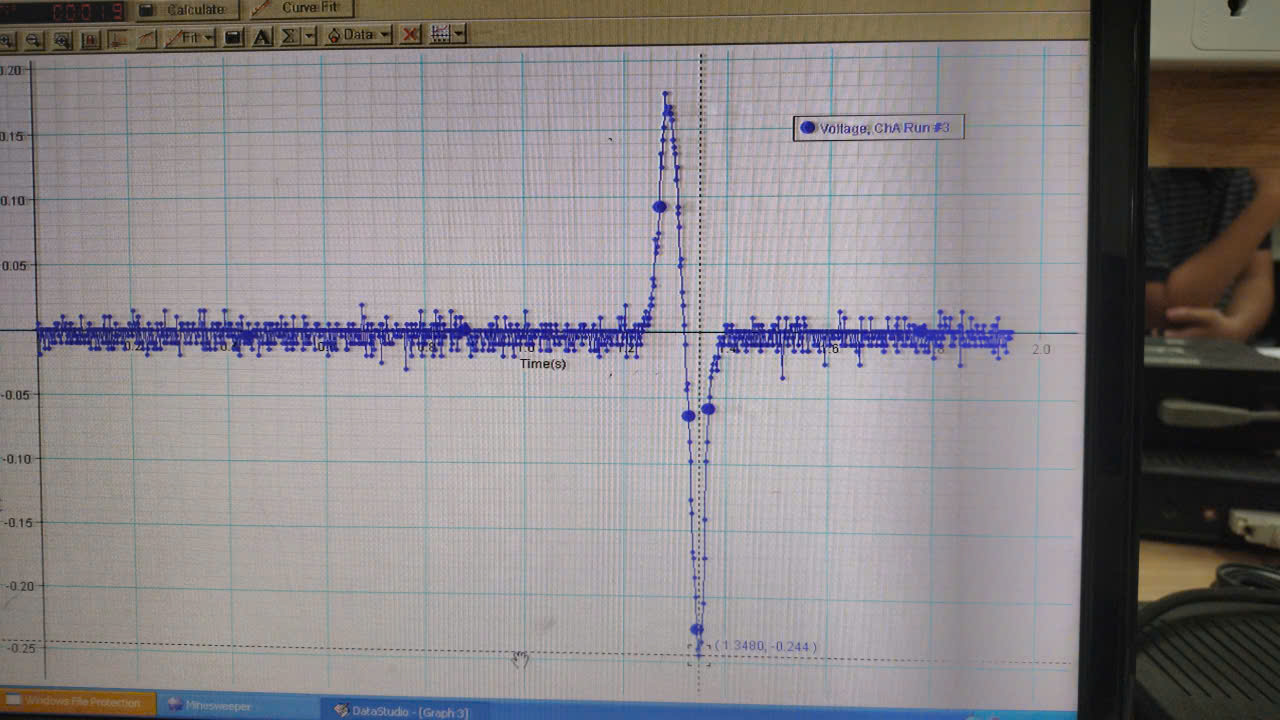
\includegraphics[width=0.95\textwidth]{150 NN.jpg}
		\captionof{figure}{\textit{North-North down}}
	\end{center}
	
	\subsubsection*{4.2.2. Data Table of Induced Voltage}
	\begin{table}[H]
		\centering
		\caption{Measurement results for 150-turn coil}
		\begin{tabular}{lccc}
			\toprule
			\textbf{Magnet's pole} & \textbf{Voltage peak 1 (mV)} & \textbf{Voltage peak 2 (mV)} \\
			\midrule
			North pole (N down) & $122$ & $-181$ \\
			South pole (S down) & $-142$ & $181$ \\
			Double magnet (N-S combined) & $39$ & $-73$ \\
			Double magnet (N-N / S-S) & $176$ & $-244$ \\
			\bottomrule
		\end{tabular}
	\end{table}
	
	\section*{5. Comments and explanations}
	
	\begin{bt}
		\textbf{Why is the value of the first voltage peak smaller than that of the second voltage peak?}
		
		When the magnet bar is falling, the gravity acts on it with an acceleration g. Neglecting the air resistance, we have the velocity formula
		\begin{equation}
			v\left(t\right)\approx v_0+gt\approx gt
		\end{equation}
		\qquad Let $t_1$ be the time the magnet bar just enters the coil, and $t_2$ be the time the magnet just leaves the coil. Obviously, we have
		\begin{equation}
			t_1\ <\ t_2\Longrightarrow \left(t_1\right)\ <\ v\left(t_2\right)\Longrightarrow\left|\Delta B_1\right|<\left|\Delta B_2\right|\Longrightarrow\left|V_1\right|=\left|-N\frac{\Delta B_1A}{\Delta t}\right|<\left|-N\frac{\Delta B_2A}{\Delta t}\right|=\left|V_2\right|
		\end{equation}
		where $\Delta B_1\ \text{\ and\ }\ \Delta B_2$ are the changes in the magnetic field when the magnet bar just enters and leaves the coil, respectively. Hence, we can conclude that the value of the first voltage peak is smaller than that of the second voltage peak.
		
	\end{bt}
	
	\begin{bt}
		\textbf{Why are the signals of the induced voltage in the case of N-pole and S-pole inverse with each other?}
		
		Outside the magnet, magnetic field lines travel from the North pole to the South pole. When we flip the magnet (S-pole down), the direction of the magnetic field passing through the coil is inverted compared to the N-pole case. As a result, the direction of the induced current and the polarity of the induced voltage are reversed. Hence, the voltage signals for the N-pole and S-pole cases are opposite to each other.
	\end{bt}
	
	\begin{bt}
		\textbf{Why is the signal produced by the 1200-turn coil larger than that by the 150-turn coil?}
		
		According to Faraday's law of electromagnetic induction, the magnitude of the induced voltage is proportional to the number of turns in the coil.
		In each case (N-pole down, S-pole down, etc.), suppose that the rate of change of magnetic flux  $\frac{\Delta\Phi}{\Delta\ t}$  is the same, we have
		\begin{equation}
			\left|V_{induced}^{1200-turn\ coil}\right|\ =\ \left|-1200\ \frac{\Delta\Phi}{\Delta t}\right|>\left|-150\ \frac{\Delta\Phi}{\Delta t}\right|=\left|V_{induced}^{150-turn\ coil}\right|
		\end{equation}
		
		Therefore, the signal produced by a 1200-turn coil is larger than that by a 150-turn coil.
		
	\end{bt}
	
	\begin{bt}
		\textbf{What is your comment for the case when you use the set of two magnets for the measurement performed at step 7 and 8?}
		
		Step 7 (Opposite poles aligned): The magnetic fields of both magnet bars cancel each other out, making the net flux change close to zero. As a result, the induced voltage is nearly zero.
		
		Step 8 (Same poles aligned): Roughly doubles the magnetic field strength, thereby roughly doubling the rate of change of flux and doubling the peak induced voltage.
		
	\end{bt}
	

%% =====================================================================
%% EXPERIMENT 5  (content copied unchanged from Ex5-prefinal.tex)
%% =====================================================================
\StartExperiment{5}{Investigation of Transmission of Electromagnetic Wave (Microwave)}
	\renewcommand{\figurename}{Figure}
	\renewcommand{\tablename}{Table}
	
	\begin{center}
		\textbf{\Large EXPERIMENT 5}
		
		\vspace{0.5cm}
		\textbf{{\Large INVESTIGATION OF TRANSMISSION OF}}
		
		\vspace{0.25cm}
		\textbf{{\Large ELECTROMAGNETIC WAVE (MICROWAVE)}}
	\end{center}
	
	\section*{1.  Devices and Purpose of the experiment}
	\begin{center}
		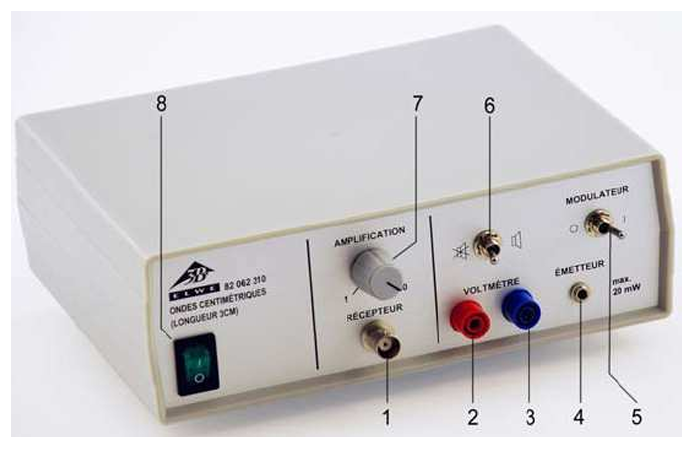
\includegraphics[width=0.5\textwidth]{Devices51}
		\captionof{figure}{\textit{ Control unit, (1) receiver terminal, (2) amplifier output, (3) amplifier output (ground); (4) transmitter terminal, (5) modulator switch, (6) speaker switch, (7) amplifier gain (amplification), (8) mains switch}}
	\end{center}
	\begin{center}
		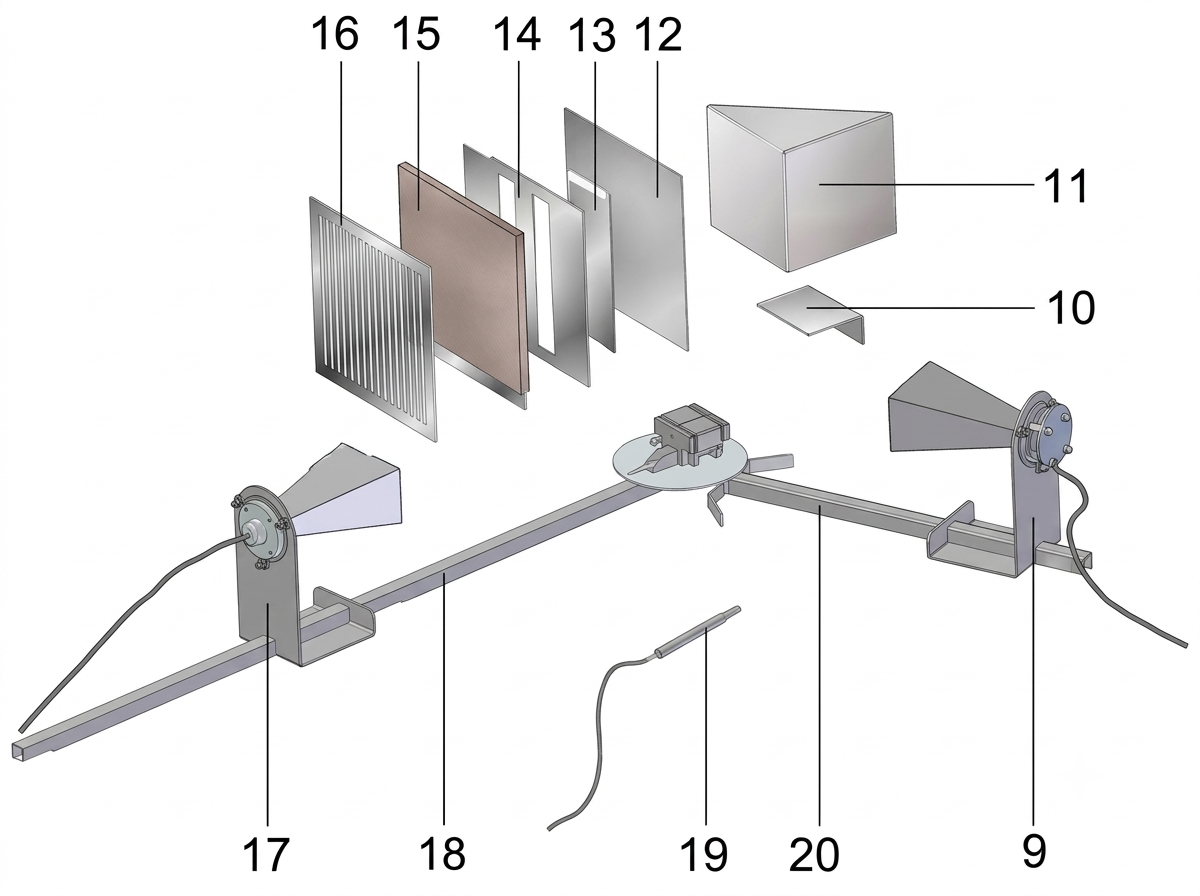
\includegraphics[width=0.6\textwidth]{Devices52}
		\captionof{figure}{\textit{ Accessories: (9) transmitter with horn antenna, (10) stand for prism, (11) paraffin prism; (12) reflection plate. (13) cover plate for double slit, (14) plate with double slit. (15) absorption plate, (16) polarization grating, (17) receiver with horn antenna, (18) microwave bench, (19) microwave probe, (20) folding microwave bench with plate holder}}
	\end{center}
	
	
	
	\section*{2. Theoretical background}
	Microwaves are radio waves belonging to the electromagnetic (EM) spectrum whose wavelengths are conveniently measured in a few centimeters, corresponding to frequencies ranging from roughly $1.0\text{ GHz}$ to $30\text{ GHz}$. The small wavelength of microwaves allows conveniently sized antennas to direct them in narrow beams, which can be pointed directly at the receiving antenna.
	
	\vspace{0.3cm}
	\noindent
	Microwave radio transmission is commonly used:
	\begin{itemize}[leftmargin=1.5em]
		\item In point-to-point communication systems on the surface of the Earth, in satellite communications, and in deep-space radio communications.
		\item For radars, radio navigation systems, sensor systems, and radio astronomy.
	\end{itemize}
	
	\vspace{0.2cm}
	\noindent
	The components and equipment included allow various experiments to be performed. A narrow beam of electromagnetic waves with a wavelength in the centimeter range (microwaves) in the form of a square-modulated signal is generated by the control unit, output by a transmitter, and picked up using accessories such as a horn antenna or a sensor probe. The modulation of the received signal can be rendered audible by means of an internal speaker, and the intensity of the signal can also be controlled.
	
	\section*{3. Experimental procedure}
	\subsection*{3.1. Straight-line propagation of microwaves}
	\begin{center}
		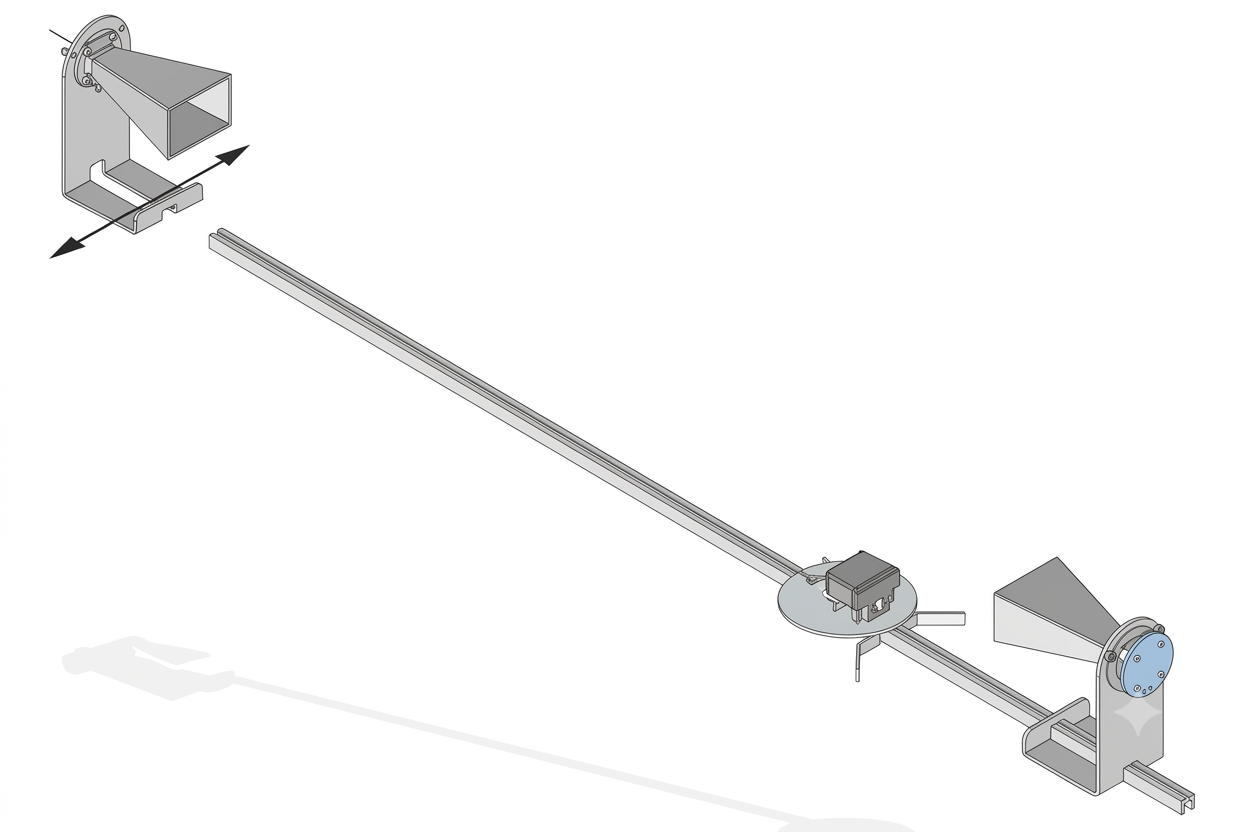
\includegraphics[width=0.5\textwidth]{Fig1}
		\captionof{figure}{\textit{Experimental setup for straight-line propagation of microwaves}}
	\end{center}
	\begin{enumerate}[leftmargin=1.5em]
		\item Set up the transmitter and receiver facing one another with the receiver off the rail, as shown in Fig. 1.
		\item Move the receiver in a plane perpendicular to the rail. Observe and draw a conclusion on the optimum position of the horns for reception.
	\end{enumerate}
	
	\subsection*{3.2. Penetration of microwaves}
	\begin{center}
		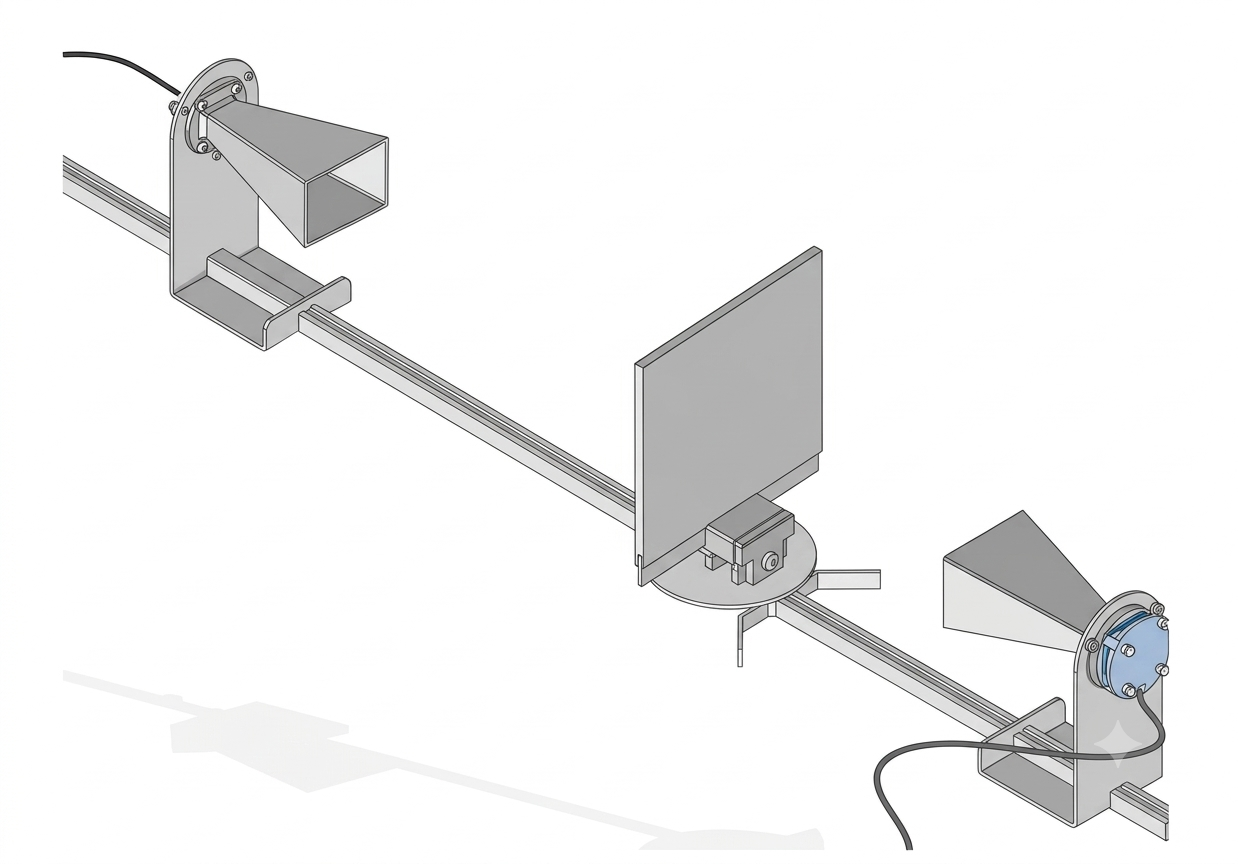
\includegraphics[width=0.5\textwidth]{Fig2}
		\captionof{figure}{\textit{Experimental setup for penetration of microwaves}}
	\end{center}
	\begin{enumerate}[leftmargin=1.5em]
		\item Set up the transmitter and receiver facing one another.
		\item Attach the dry absorption plate (electrical insulator) to the plate holder and place it between the transmitter and receiver, as shown in Fig. 2.
		\item Set the amplification to a medium level. Observe and draw a conclusion on the reception of the signal.
	\end{enumerate}
	
	\subsection*{3.3. Screening and absorption of microwaves}
	\begin{center}
		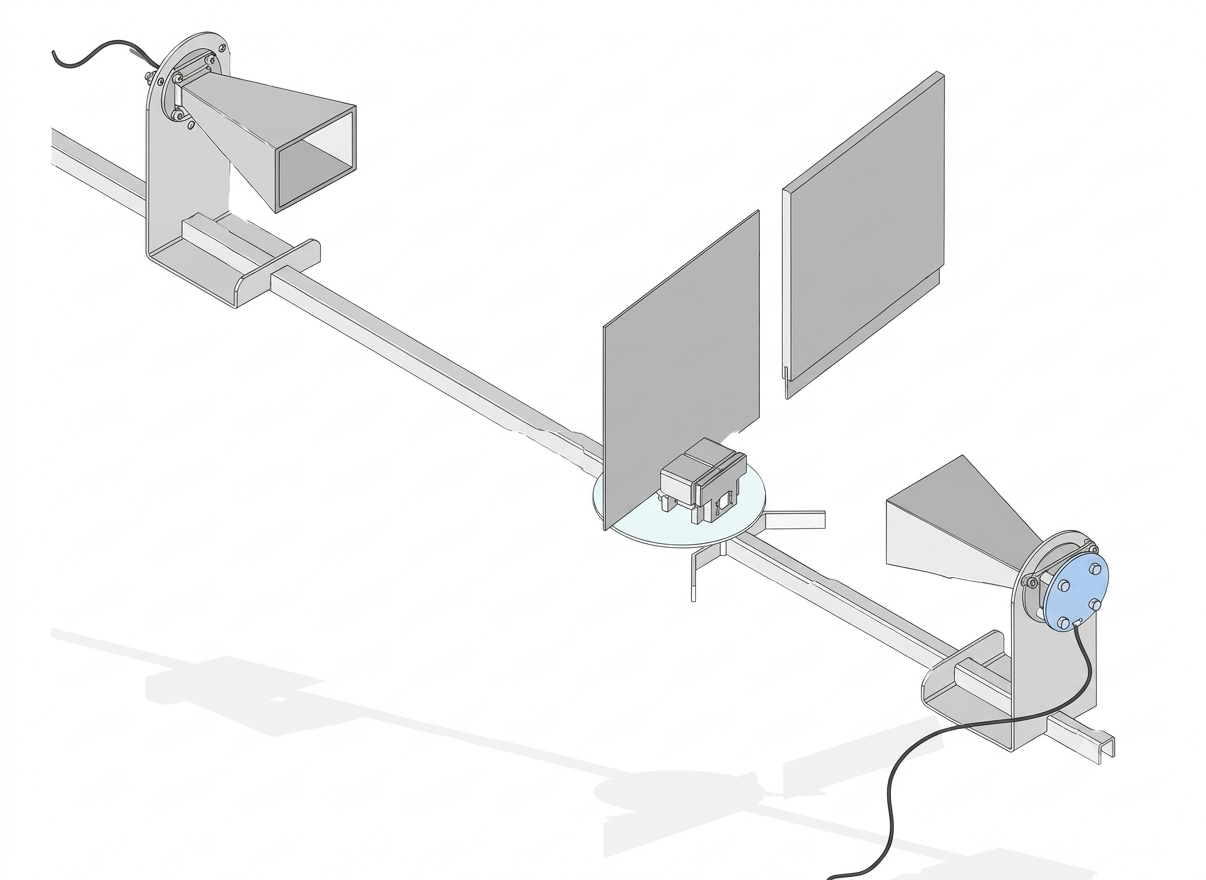
\includegraphics[width=0.5\textwidth]{Fig3}
		\captionof{figure}{\textit{Experimental setup for screening and absorption of microwaves}}
	\end{center}
	\begin{enumerate}[leftmargin=1.5em]
		\item Set up the transmitter and receiver facing one another.
		\item Place the reflection plate (electrical conductor) between the transmitter and receiver as shown in Fig. 3.
		\item Set the amplification to a medium level. Observe and draw a conclusion on the reception of the signal.
		\item Replace the reflection plate with the absorption plate. Observe and draw a conclusion on the reception of the signal.
	\end{enumerate}
	
	\subsection*{3.4. Reflection of microwaves}
	\begin{center}
		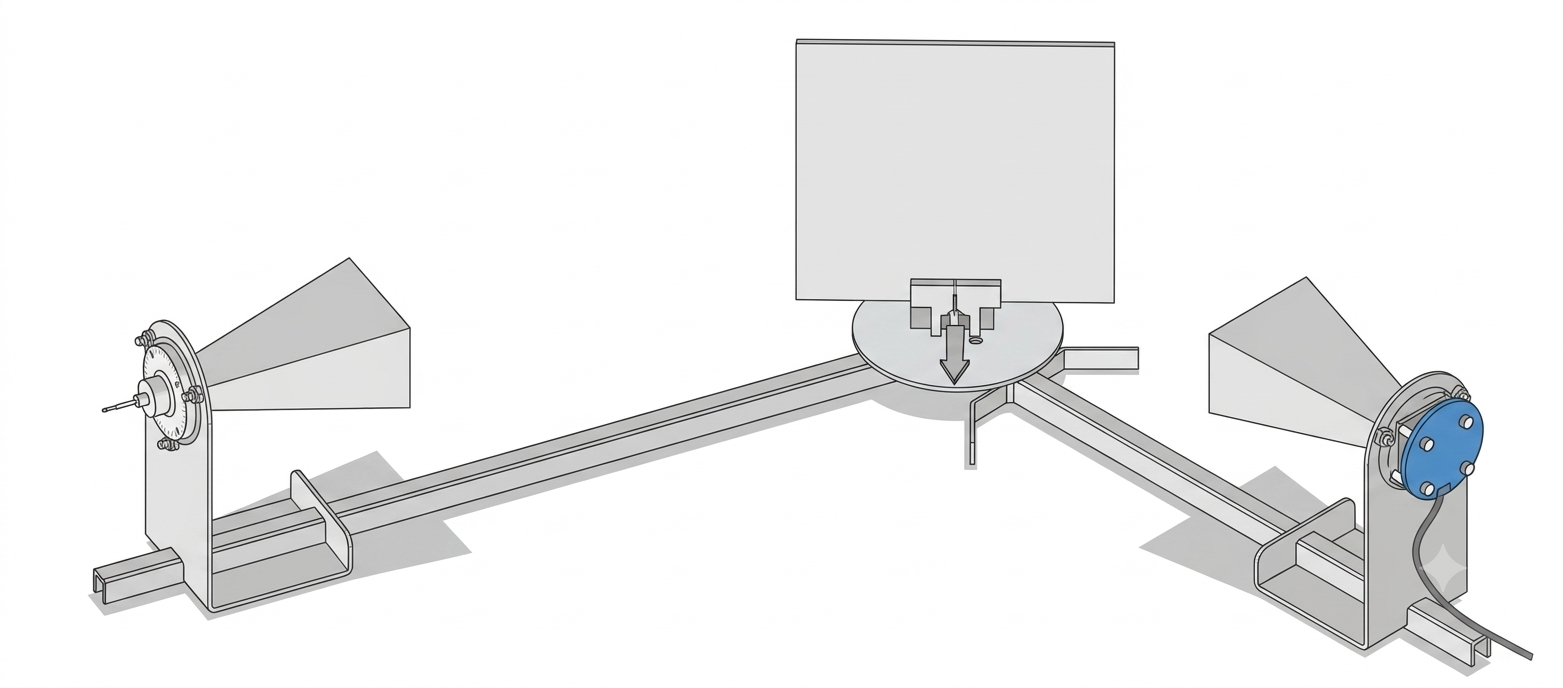
\includegraphics[width=0.5\textwidth]{Fig4}
		\captionof{figure}{\textit{Experimental setup for reflection of microwaves}}
	\end{center}
	\begin{enumerate}[leftmargin=1.5em]
		\item Set up the transmitter and receiver so that the angle of incidence can be read off.
		\item Line up the reflector plate at an angle of approximately $30^\circ$ with the help of the pointer for the rails, which points in the direction of the normal (a line perpendicular to the mirror's surface), as shown in Fig. 4.
		\item Change the angle of the long rail until maximum reception is attained. Measure the angles of incidence and reflection from the normal (arrow) and draw a conclusion.
		\item Repeat the procedure with other angles of the reflector, namely $40^\circ$, $50^\circ$, and $60^\circ$.
	\end{enumerate}
	
	\subsection*{3.5. Refraction of microwaves}
	\begin{center}
		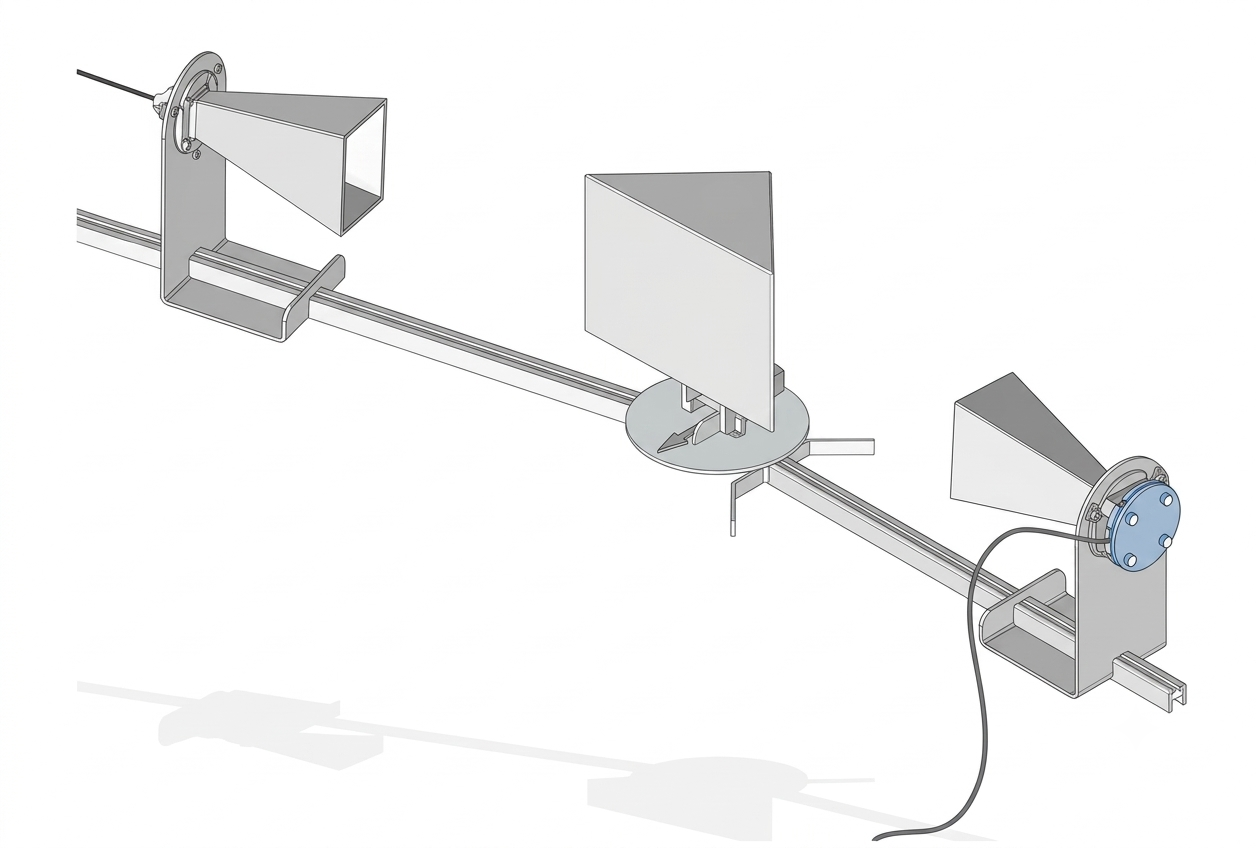
\includegraphics[width=0.5\textwidth]{Fig5}
		\captionof{figure}{\textit{Experimental setup for refraction of microwaves}}
	\end{center}
	\begin{enumerate}[leftmargin=1.5em]
		\item Set up the accessories including the transmitter, receiver, and prism on its stand facing away from the arrow, as shown in Fig. 5.
		\item Turn the long rail until maximum reception is attained. Observe and draw a conclusion on the reception of the signal.
	\end{enumerate}
	
	\subsection*{3.6. Diffraction of microwaves}
	\begin{center}
		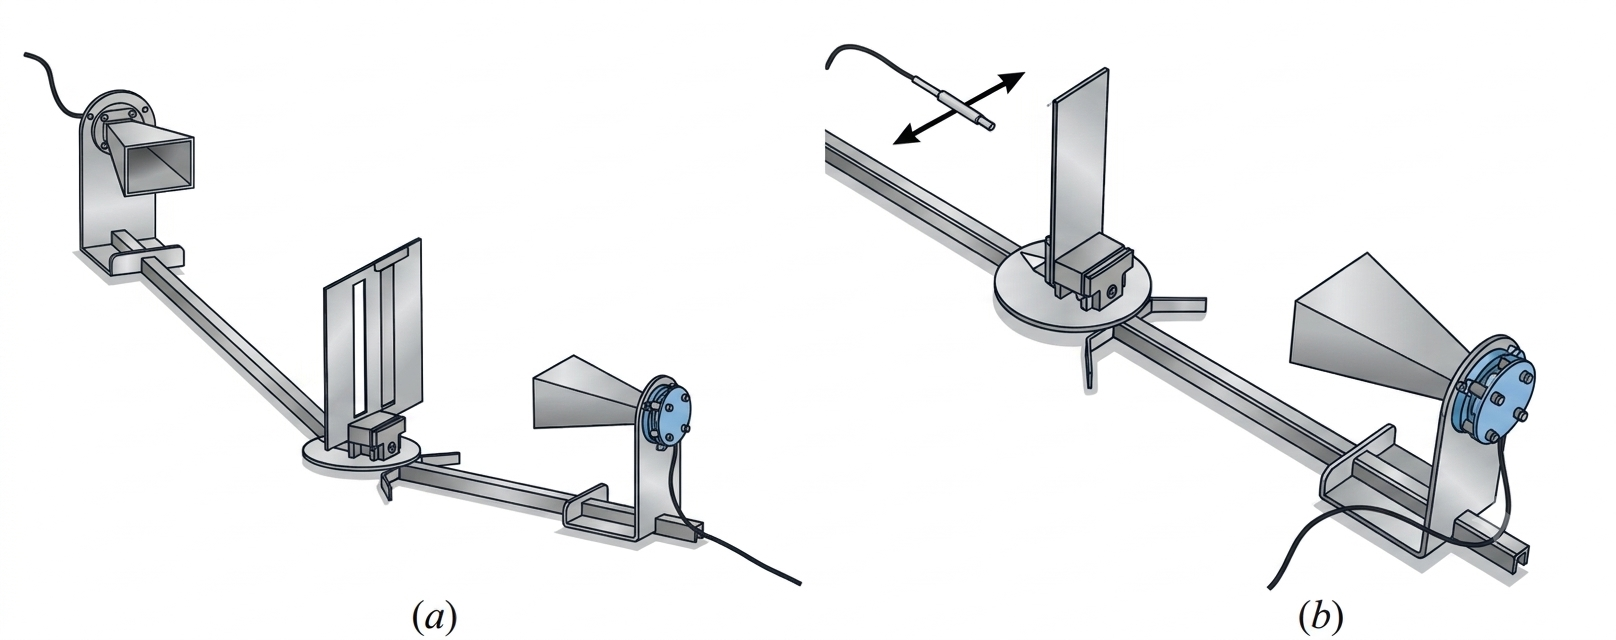
\includegraphics[width=0.8\textwidth]{Fig6}
		\captionof{figure}{\textit{Experimental setup for diffraction of microwaves}}
	\end{center}
	\begin{enumerate}[leftmargin=1.5em]
		\item Set up the accessories including the transmitter and receiver directly facing each other about $80\text{ cm}$ apart, as shown in Fig. 6a. Turn the receiver around on its rail so that it is out of the bundled microwave beam and the signal is clearly weakened.
		\item Place the single-slit plate (with the slit width smaller than the wavelength) vertically aligned about $20\text{ cm}$ in front of the transmitter so that the receiver once more detects a signal.
		\item Observe and draw a conclusion on the reception of the signal showing that microwaves are diffracted by the slit and wavelets can be detected in the shadow of the aperture.
		\item Clamp the cover plate in the holder on the hinge plate and set up the transmitter about $20\text{ cm}$ in front of the plate, as shown in Fig. 6b.
		\item Move the probe in a horizontal plane behind the plate. Observe and record the corresponding signal on the multimeter. Draw conclusions from the experimental results, especially when the probe is in the shadow of the plate.
	\end{enumerate}
	
	\subsection*{3.7. Interference of microwaves}
	\begin{center}
		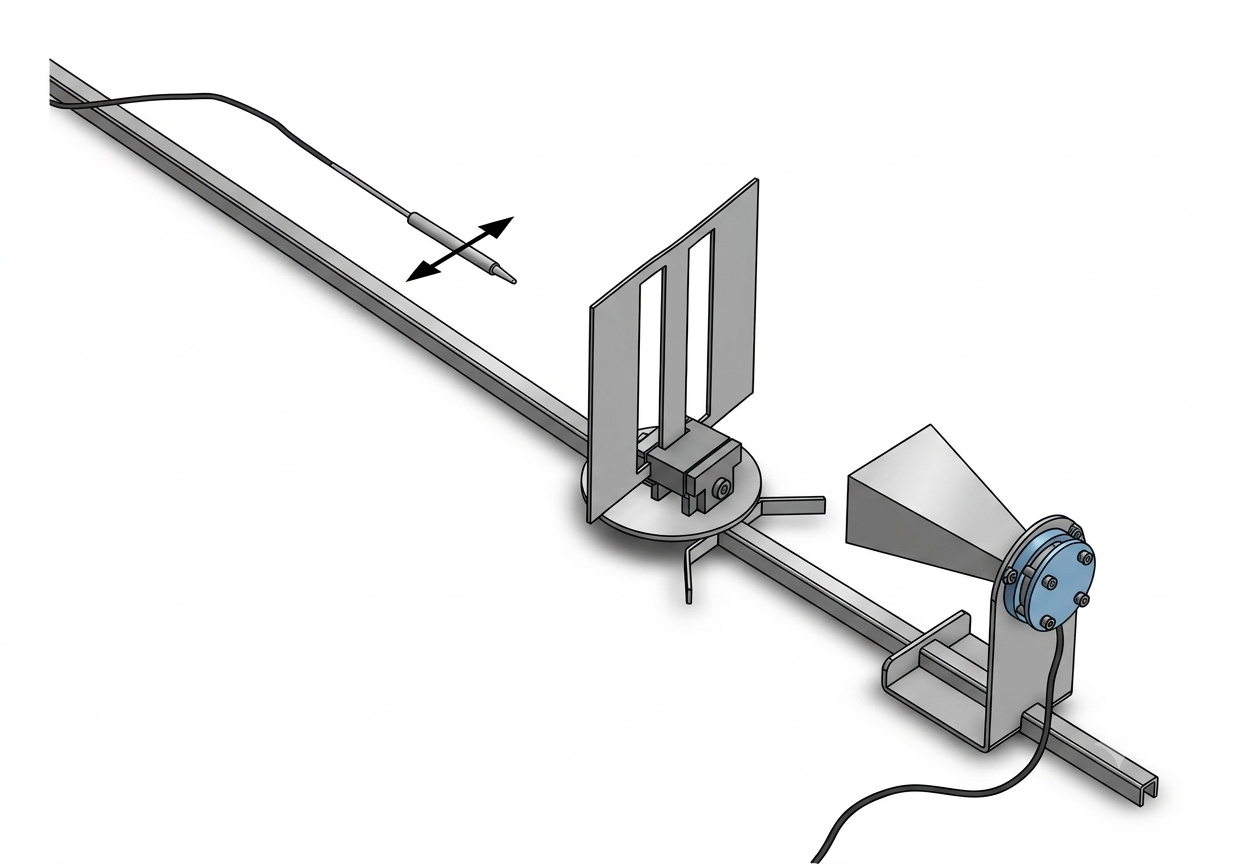
\includegraphics[width=0.5\textwidth]{Fig7}
		\captionof{figure}{\textit{Experimental setup for interference of microwaves}}
	\end{center}
	\begin{enumerate}[leftmargin=1.5em]
		\item Clamp the plate with the double slit centrally in the holder on the plate over the hinge. Position the transmitter about $12\text{ cm}$ in front of the plate. Place the receiver probe, which is connected to a multimeter, about $6\text{ cm}$ behind the double-slit plate, as shown in Fig. 7.
		\item Move the receiver probe parallel to the double-slit plate, as illustrated in Fig. 7. Observe and record the number of interference maxima corresponding to the signal on the digital multimeter. Draw conclusions from the experimental results.
	\end{enumerate}
	
	\subsection*{3.8. Polarization of microwaves}
	\begin{center}
		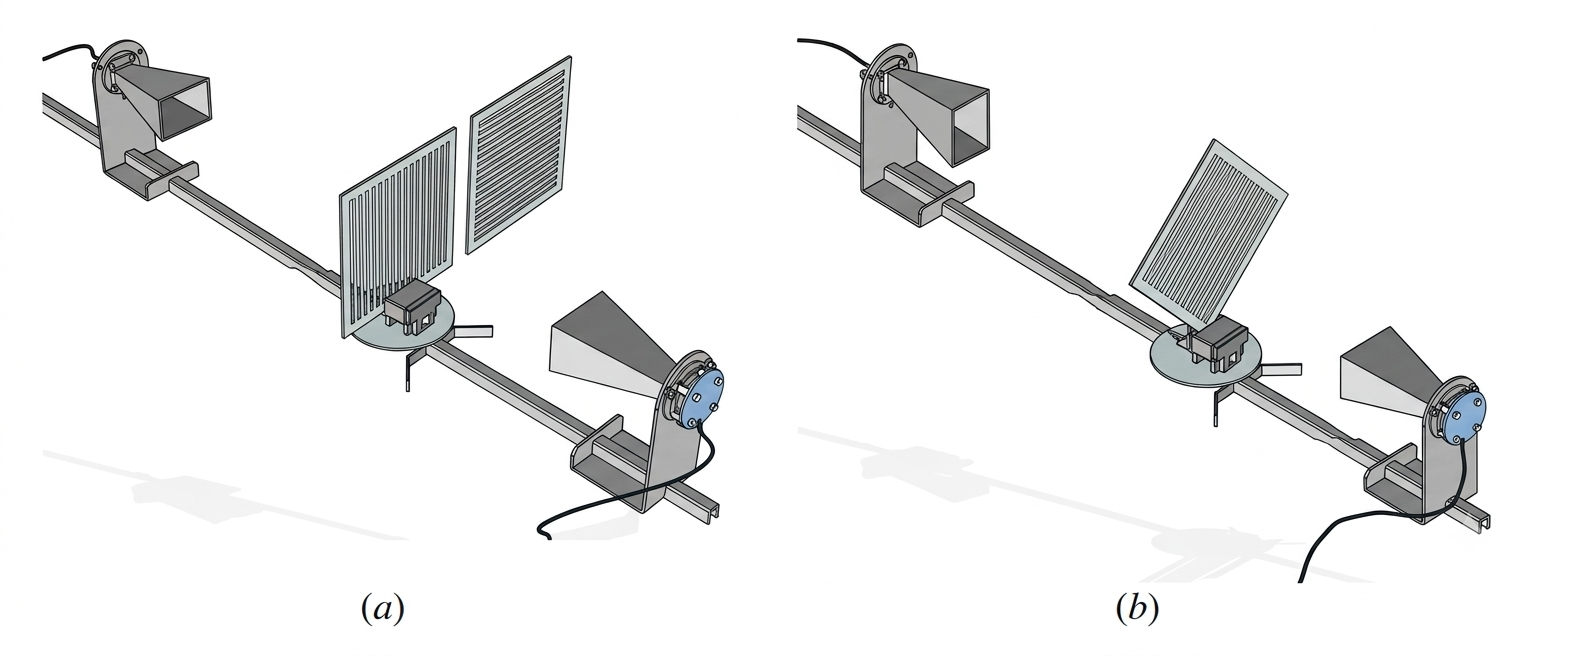
\includegraphics[width=0.8\textwidth]{Fig8}
		\captionof{figure}{\textit{Experimental setup for polarization of microwaves}}
	\end{center}
	\begin{enumerate}[leftmargin=1.5em]
		\item Set up the polarization grating in the screen holder.
		\item Check the reception when the polarization grating is aligned horizontally and vertically, as illustrated in Fig. 8a. Draw conclusions about the receiver's signal and provide explanations for the experimental results in both cases.
		\item Check the reception when the polarization grating is introduced into the beam and tilted by $45^\circ$, as shown in Fig. 8b. Draw conclusions about the receiver's signal and explain the experimental results.
	\end{enumerate}
	
	\subsection*{3.9. Wavelength of standing waves}
	\begin{center}
		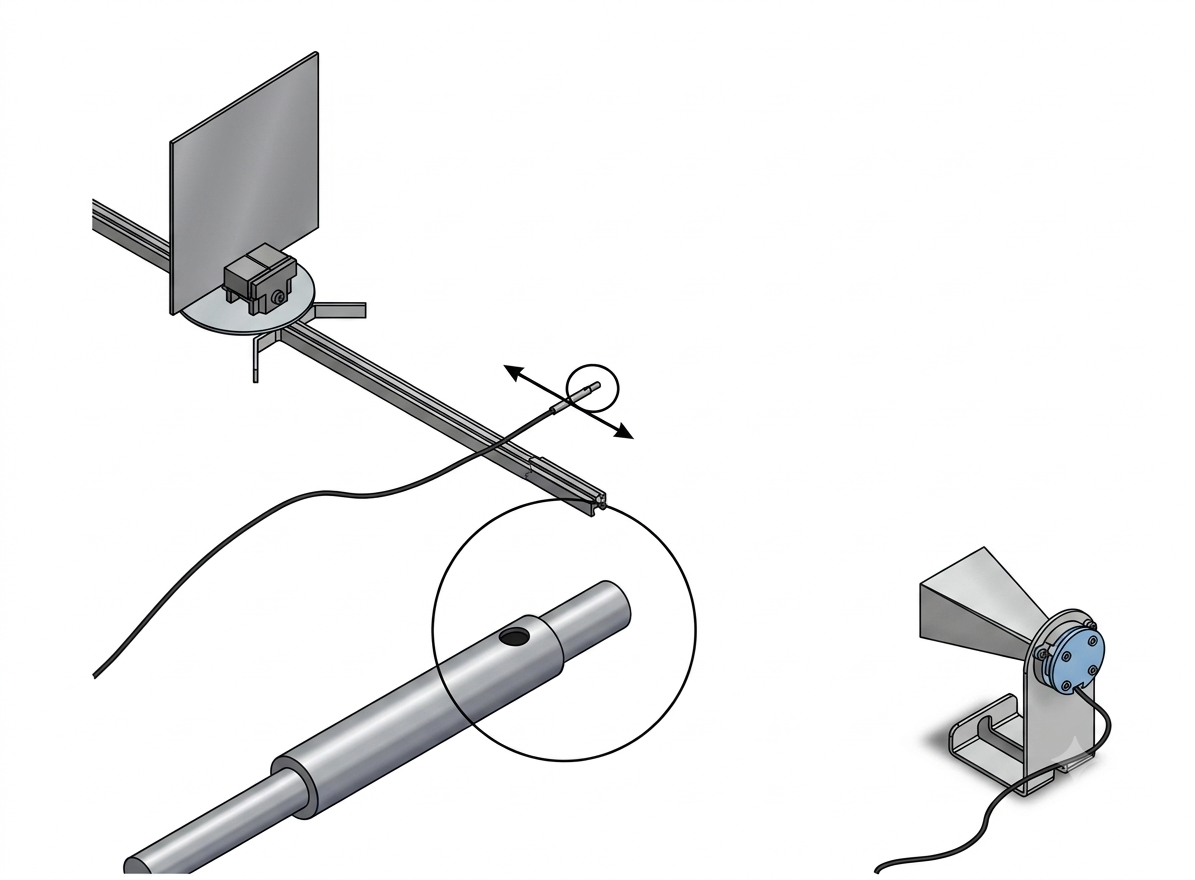
\includegraphics[width=0.5\textwidth]{Fig9}
		\captionof{figure}{\textit{Experimental setup for measuring the wavelength of standing waves}}
	\end{center}
	Set up the transmitter and reflector plate facing each other about $50\text{ cm}$ apart (in this case, the angle of incidence is $0^\circ$), as shown in Fig. 11. The transmitted and reflected waves are superimposed, resulting in a standing wave such that the wavelength corresponds to twice the distance between two adjacent minima (or maxima), i.e., $\lambda = 2d$.
	\begin{enumerate}[leftmargin=1.5em]
		\item Roughly investigate the interference maxima and minima of the transmitted and reflected waves by moving the microwave probe on the surface of and along the long bench, as illustrated in Fig. 9.
		\item Place the probe at the position corresponding to an interference maximum (or minimum) by observing the display on the voltmeter, and record that position as $x_1$. Afterward, continue moving the probe to the adjacent position of an interference maximum (or minimum) and record that position as $x_2$. Consequently, determine the distance between these two positions as $d = |x_2 - x_1|$.
		\item Repeat Step 2 two more times and record the measurement results in a data table with 4 columns: Trial, $x_1$, $x_2$, and $d$, respectively.
	\end{enumerate}
	
	\section*{4. Experimental results}
	
	\subsection*{4.1. Investigation of straight-line propagation of microwaves}
	\noindent
	When the receiver is aligned with the rail (the transmitter and the receiver are facing each other), the volt-meter shows the maximum value.
	
	\noindent
	When the receiver moves far from the rail (in a plane perpendicular to the rail), the value showed on the volt-meter decreases.
	
	\noindent
	Hence, microwaves propagate best in a straight line.
	\subsection*{4.2. Investigation of penetration of microwaves}
	\noindent
	When a dry absorption plate is put between the transmitter and the receiver, the value showed on the volt-meter slightly decreases.
	
	\noindent
	We can conclude that microwaves can penetrate through the dry absorption plate, but not all of the microwaves will penetrate through the dry absorption plate. Instead, a part of them will be absorbed by the absorption plate.
	
	\subsection*{4.3. Investigation of screening and absorption of microwaves}
	\noindent
	When a reflection plate is put between the transmitter and the receiver, the volt-meter shows a value close to 0 (0.01). It implies that the reflection plate screens the microwaves by reflecting them, preventing them from passing through.
	
	\subsection*{4.4. Investigation of reflection of microwaves}
	\noindent
	After trying multiple reflector angles, we yield a data table recording the incidence angles making the volt-meter show maximum value.
	\begin{table}[H]
		\centering
		\begin{tabular}{|>{\centering\arraybackslash}m{1.5cm}|>{\centering\arraybackslash}m{4.5cm}|>{\centering\arraybackslash}m{4.5cm}|}
			\hline
			\textbf{Trial} & \textbf{Reflector angle$\left(^\circ\right)$} & \textbf{Incidence angle$\left(^\circ\right)$} \rule[-0.2cm]{0pt}{0.6cm} \\
			\hline
			1 & 30 & 30 \rule[-0.25cm]{0pt}{0.7cm} \\
			\hline
			2 & 40 & 40 \rule[-0.25cm]{0pt}{0.7cm} \\
			\hline
			3 & 50 & 50 \rule[-0.25cm]{0pt}{0.7cm} \\
			\hline
			4 & 60 & 60 \rule[-0.25cm]{0pt}{0.7cm} \\
			\hline
		\end{tabular}
	\end{table}
	\noindent
	Hence, we can conclude that microwaves reflects best when the perpendicular bisector of the reflection plate is the  bisector  of  an  angle  created  by  the  transmitter  and  receiver; and when the microwaves reflect, the angle of incidence equals the angle of reflection.
	
	
	\subsection*{4.5. Investigation of refraction of microwaves}
	\noindent
	When the angle created by 2 rails is $150^\circ$, the volt-meter shows the maximum value. Turning the receiver to a different angle makes the value showed on the volt-meter decreases.
	
	\noindent
	We can conclude that: When microwaves pass through the paraffin prism, they undergo refraction (bending). The angle of $150^\circ$ corresponds to the angle of deviation where the refracted beam has the highest intensity.
	
	\subsection*{4.6. Investigation of diffraction of microwaves}
	\noindent
	When the single slit plate is put in the rail, the value showed on the volt-meter increases.
	
	\noindent
	When the cover plate is between the probe and the transmitter, the value showed on the volt-meter is approximate 0 in the shadow. When the probe is moved on the horizontal plane behind the plate, the value slightly increases.
	
	\noindent
	All evidences show that microwaves diffract. They curve around the edges of an obstacle (like a cover plate) and spread into the shadow region after traveling through a single-slit opening.
	
	\subsection*{4.7. Investigation of interference of microwaves}
	\noindent
	When the probe is moved parallel to the plate, the value showed on the volt-meter is oscillating. The number of interference maxima is 3. It implies that microwaves have the property of interference.
	
	\subsection*{4.8. Investigation of polarization of microwaves}
	\noindent
	When the grating is aligned horizontally, the value showed on the volt-meter almost unchanges.
	
	\noindent
	When the grating is aligned vertically, the value showed on the volt-meter is approximate to $0$.
	
	\noindent
	When the grating is aligned at $45^\circ$, the value showed on the volt-meter is higher than that in vertical case, but lower than that in horizontal case.
	
	\noindent
	These results demonstrate that microwaves are transverse, linearly polarized waves (polarized vertically in this setup), and their transmission through a polarizing grating depends on the angle between the grating bars and the wave's plane of polarization.
	
	
	\subsection*{4.9. Wavelength and Frequency of Microwaves}
	\subsubsection*{4.9.1. Data Table}
	
	\begin{table}[H]
		\centering
		\caption{Measurement of standing wave positions}
		\begin{tabular}{|>{\centering\arraybackslash}m{1.5cm}|>{\centering\arraybackslash}m{4cm}|>{\centering\arraybackslash}m{4cm}|>{\centering\arraybackslash}m{4cm}|}
			\hline
			\textbf{Trial} & \textbf{$x_1$ (mm)} & \textbf{$x_2$ (mm)} & \textbf{$d$ (mm)} \rule[-0.2cm]{0pt}{0.6cm} \\
			\hline
			1 & 160 & 175 & 15 \rule[-0.25cm]{0pt}{0.7cm} \\
			\hline
			2 & 175 & 190 & 15 \rule[-0.25cm]{0pt}{0.7cm} \\
			\hline
			3 & 190 & 206 & 16 \rule[-0.25cm]{0pt}{0.7cm} \\
			\hline
		\end{tabular}
	\end{table}
	
	\subsubsection*{4.9.2. Data Processing}
	
	\noindent
	The mean value of $d$ is
	\begin{center}
		\fbox{%
			\begin{minipage}{0.8\textwidth}
				\vspace{-0.4cm}
				\centering
				\begin{displaymath}
					\overline{d} = \frac{d_1 + d_2 + d_3}{3} = \dfrac{46}{3} \left(\text{mm}\right)
				\end{displaymath}
			\end{minipage}%
		}
	\end{center}
	
	\noindent
	The standard deviation of a single measurement is
	\begin{center}
		\fbox{%
			\begin{minipage}{0.8\textwidth}
				\vspace{-0.4cm}
				\centering
				\begin{displaymath}
					\text{sd}_d = \sqrt{\frac{\left(d_1 - \overline{d}\right)^2 + \left(d_2 - \overline{d}\right)^2 + \left(d_3 - \overline{d}\right)^2}{3}} = \dfrac{\sqrt{2}}{3} \left(\text{mm}\right)
				\end{displaymath}
			\end{minipage}%
		}
	\end{center}
	
	\noindent
	And the standard deviation of the mean is
	\begin{center}
		\fbox{%
			\begin{minipage}{0.8\textwidth}
				\vspace{-0.4cm}
				\centering
				\begin{displaymath}
					\text{SD}_d = \frac{\text{sd}_d}{\sqrt{3}} = \dfrac{\sqrt{6}}{9} \left(\text{mm}\right)
				\end{displaymath}
			\end{minipage}%
		}
	\end{center}
	
	\noindent
	Using $\lambda = 2d$, the mean wavelength and its uncertainty are
	\begin{center}
		\fbox{%
			\begin{minipage}{0.8\textwidth}
				\vspace{-0.4cm}
				\centering
				\begin{displaymath}
					\begin{aligned}
						&\overline{\lambda} = 2\overline{d} = \dfrac{92}{3} \left(\text{mm}\right) \approx 30.667  \left(\text{mm}\right) \\
						&\Delta \lambda = 2\,\text{SD}_d = \dfrac{2\sqrt{6}}{9} \left(\text{mm}\right) \approx 0.544  \left(\text{mm}\right)
					\end{aligned}
				\end{displaymath}
			\end{minipage}%
		}
	\end{center}
	
	\noindent
	Therefore, our result for $\lambda$ appears as
	\begin{center}
		\fbox{%
			\begin{minipage}{0.8\textwidth}
				\vspace{-0.4cm}
				\centering
				\begin{displaymath}
					\lambda = \overline{\lambda} \pm \Delta \lambda = 30.667 \pm 0.544 \left(\text{mm}\right)
				\end{displaymath}
			\end{minipage}%
		}
	\end{center}
	
	\noindent
	Using $c = \lambda f$ with $c = 3 \times 10^8\text{ m/s}$, the mean frequency and its uncertainty are
	\begin{center}
		\fbox{%
			\begin{minipage}{0.8\textwidth}
				\vspace{-0.4cm}
				\centering
				\begin{displaymath}
					\begin{aligned}
						&\overline{f} = \frac{c}{\overline{\lambda}} = \dfrac{3 \times 10^8}{\dfrac{92}{3} \times 10^{-3}} = \dfrac{900}{92} \times 10^9 \approx 9.783 \times 10^9 \left(\text{Hz}\right) \\
						&\Delta f = \overline{f} \cdot \frac{\Delta \lambda}{\overline{\lambda}} = \dfrac{900}{92} \times 10^9 \times \dfrac{\dfrac{2\sqrt{6}}{9} \times 10^{-3}}{\dfrac{92}{3} \times 10^{-3}} \approx 0.174 \times 10^9 \left(\text{Hz}\right)
					\end{aligned}
				\end{displaymath}
			\end{minipage}%
		}
	\end{center}
	
	\noindent
	Therefore, our result for $f$ appears as
	\begin{center}
		\fbox{%
			\begin{minipage}{0.8\textwidth}
				\vspace{-0.4cm}
				\centering
				\begin{displaymath}
					f = \overline{f} \pm \Delta f = \left(9.783 \pm 0.174\right) \times 10^9 \left(\text{Hz}\right)
				\end{displaymath}
			\end{minipage}%
		}
	\end{center}
	

\end{document}
